%%%%%%%%%%%%%%%%%%%%%%%%%%%%%%%%%%%%%%%%%%%%%%%%%%%%%%%%%%%%%%%%%%%%%%
% Lớp 11 | Đường thẳng, mặt phẳng. Quan hệ song song trong | Điểm, đường thẳng và mặt phẳng
% Dạng 1H4?1-4: Tìm giao điểm của đường thẳng và mặt phẳng
% Số câu: 76  (sinh tự động bởi tach_cau.py; từ nay thầy sửa trực tiếp file này)
%%%%%%%%%%%%%%%%%%%%%%%%%%%%%%%%%%%%%%%%%%%%%%%%%%%%%%%%%%%%%%%%%%%%%%

%%%%%%%%%%%%%%%% TRẮC NGHIỆM 4 PHƯƠNG ÁN %%%%%%%%%%%%%%%%

% nguồn: Ok_Toan11_TracNghiem_Lan2
\begin{ex}%[1H4N1-4]%[ma:8ea28719]
	Cho hình chóp $S.ABCD$, đáy $ABCD$ là hình bình  hành, điểm $M$ thuộc cạnh $SA$ sao cho $AM=\dfrac{1}{3}SA$, điểm $N$ thuộc cạnh $SC$ sao cho $SN=\dfrac{3}{4}SC$. Đường thẳng $MN$ cắt đường thẳng nào trong các đường sau?
	\choice 
		 {$SB$}
		{$BD$} 
		 {$AD$}
		{\True  $AC$}
	\loigiai{ 
	 \immini
		{Xét tam giác $SAC$ ta  có $SM=\dfrac{2}{3}SA$ suy ra $\dfrac{SM}{SA}=\dfrac{2}{3}$.\\
		 Ta có $SN=\dfrac{3}{4} SC$ suy ra $\dfrac{SN}{SC}=\dfrac{3}{4}$.\\
		Do $\dfrac{SM}{SA} \ne \dfrac{SN}{SC}$ nên  $MN$, $AC$ không song song.\\
		Do đó $MN$ và  $AC$ cắt nhau.}
		{\begin{tikzpicture}[scale=1,font=\footnotesize,line join=round,line cap=round,>=stealth]
		\path (0,0) coordinate  (A)+(-150:1.5) coordinate (D)
			(2.5,0) coordinate (B)+(-150:1.5) coordinate  (C)
			(70:2) coordinate  (S)
			($(S)!2/3!(A)$) coordinate (M) 
			($(S)!3/4!(C)$) coordinate (N); 
		 \draw (S)--(D)--(C)--(B)--cycle (D)--(S)--(C);
		 \draw[dashed] (C)--(A)--(B)
			(M)--(N) 
			(D)--(A)--(S); 
		\foreach \x/\g in  {S/90,A/180,B/0,C/-90,D/-135,M/180,N/45}{\fill (\x) circle (1pt)+(\g:0.3) node{$\x$};}
	\end{tikzpicture}
		} 
	} 
\end{ex}

% nguồn: Ok_Toan11_TracNghiem_Lan2
\begin{ex}%[1H4H1-4]%[ma:215ed4d9]
	Cho hình chóp $S. ABCD$ có đáy là hình bình hành. Gọi $M, I$ lần lượt là trung điểm  của $SA, BC$ điểm $G$ nằm giữa $S$ và $I$ sao cho $\dfrac{SG}{SI}=\dfrac{3}{5}$. Tìm giao điểm của đường thẳng $MG$ với mặt phẳng $(ABCD)$.
	 \choice
		{\True Là giao điểm của đường thẳng $MG$  và đường thẳng $AI$}
		 {Là giao điểm của đường thẳng $MG$ và đường thẳng $BC$}
		{Là giao  điểm của đường thẳng $MG$ và đường thẳng $CD$}
		{Là giao điểm  của đường thẳng $MG$ và đường thẳng $AB$}
	\loigiai{ 
		\begin{center}
			\begin{tikzpicture}[scale=1,font=\footnotesize,line join=round,line cap=round,>=stealth]
					 \path
						(0,0)  coordinate (A)++(0:5) coordinate (D)++(230:2) coordinate (C)++(180:5) coordinate (B)
						 (A)++(75:4) coordinate (S)
						($(B)!0.5!(C)$)  coordinate (I)
						 ($(S)!.5!(A)$) coordinate (M)
						($(S)!3/5!(I)$) coordinate  (G)
						 (intersection of M--G and A--I) coordinate (J)
						(intersection of J--G and B--C)  coordinate (J1);
					 \draw (C)--(S)--(B)--(I)--(J)
						(J1)--(C)--(D)--(S)--(B) 
						 (S)--(I)
						(G)--(J); 
					\draw[dashed] (B)--(A)--(S) 
						(D)--(A)--(I) 
						 (M)--(G)
						(I)--(J1); 
					\foreach \p/\q in  {A/180,B/180,C/-90,D/40,M/0,J/30,G/0,I/-90,S/90}
					\fill  (\p) circle (1.0pt)
						 ($(\p)+(\q:2.5mm)$) node{$\p$};
				\end{tikzpicture}
		\end{center}
		Xét trong mặt phẳng $(SAI)$  ta có $MG\cap AI=J$.\\
		Ta có $\heva{&J\in AI\subset(ABCD)\\&J\in MG}\Rightarrow MG\cap (ABCD)=J$. 
	 }
\end{ex}

% nguồn: Ok_Toan11_TracNghiem_Lan2
\begin{ex}%[1H4H1-4]%[ma:9bb248a9]
	Cho hai hình  bình hành $ABCD$ và $ABEF$ không cùng nằm trong một mặt phẳng. Gọi $O_1$, $O_2$ lần lượt là tâm của $ABCD$, $ABEF$, $M$ là trung điểm của $CD$. Chọn khẳng định \textbf{sai} trong các khẳng định sau
	\choice 
		{\True $MO_2$ cắt  $\left(BEC\right)$}
		{$O_1 O_2$  song song với $\left(BEC\right)$}
		{$O_1 O_2$  song song với $\left(EFM\right)$}
		{$O_1 O_2$ song song  với $\left(AFD\right)$}
	\loigiai{ 
		\begin{center}
			\begin{tikzpicture}[declare function={a=5; b=3; }]
					\path 
						(0,0) coordinate (A) 
						(a,0) coordinate  (B)
						(45:b) coordinate  (D)
						(-45:b) coordinate (F) 
						($(D)+(B)$) coordinate  (C)
						 ($(F)+(B)$) coordinate (E)
						($(D)!0.5!(C)$)  coordinate (M);
					\path (intersection of A--C and B--D) coordinate (O_1); 
					\path (intersection of A--E and  B--F) coordinate (O_2);
					\path  (intersection of A--M and C--F) coordinate (J);
					\draw (E)--(J)--(M)--(D)--(A)--(F)--(E); 
					\draw[dashed] (E)--(B)--(D) 
						(M)--(C)--(B)--(A)--(C)--(E)--(A)--(M) 
						(F)--(B) 
						(M)--(O_1)--(O_2)--cycle (J)--(C); 
					 \draw (M)--(A)--(O_2)
						(M)--(O_2)--(E) 
						(O_2)--(F); 
					\foreach \t/\g in {D/120,C/95,B/-90,A/210,F/-90,E/-90,M/90,O_1/-120,O_2/-90,J/0}{ 
						\draw[fill=white] (\t) circle (1pt) node[shift={(\g:9pt)},font=\scriptsize]{$ \t  $};
					} 
				\end{tikzpicture}
		\end{center}
		Gọi $J$  là giao điểm của $AM$ và $BC$.\\
		Ta có $MO_1 \parallel AD\parallel BC\Rightarrow  MO_1 \parallel CJ$.\\
		Mà $O_1$ là  trung điểm của $AC$ nên $M$ là trung điểm của $AJ$.\\
		Do đó $MO_2  \parallel EJ$. Từ đó suy ra $MO_2 \parallel \left(BEC\right)$.\\
		Vậy $MO_2$ không cắt  $\left(BEC\right)$.
	} 
\end{ex}

% nguồn: Ok_Toan11_TracNghiem_Lan2
\begin{ex}%[1H4H1-4]%[ma:55a3ee85]
	Cho hình chóp $S.ABCD$ có đáy là hình bình hành. $M$ là trung điểm của $SC$. Gọi $I$ là giao điểm của đường thẳng $AM$ với mặt phẳng $(SBD)$. Chọn khẳng định  đúng trong các khẳng định sau đây
	 \choice
		 {$IA=3IM$}
		 {$IM=3IA$}
		{$IM=2IA$} 
		 {\True $IA=2IM$}
	 \loigiai{
	 \immini{
		 Gọi $AC\cap BD=O$ thì $(SAC)\cap(SBD)=SO$.\\
		Trong mặt phẳng $(SAC)$, lấy  $AM\cap SO=I$ $\Rightarrow I=AM\cap(SBD)$.\\
		Do trong $\triangle SAC$, $AM$ và $SO$ là hai đường trung tuyến, nên $I$ là trọng tâm $\triangle SAC$.\\ 
		 Vậy $IA=2IM$.
		 }{
		\begin{tikzpicture}[scale=1,font=\footnotesize,line join=round,line cap=round,>=stealth]
				 \path
					(0,0)  coordinate (A)
					 (0.5,-2) coordinate (B)
					(5,0) coordinate (D) 
					($(B)-(A)+(D)$) coordinate  (C)
					(2,3) coordinate (S) 
					($(S)!1/2!(C)$) coordinate (M) 
					(intersection of A--C  and B--D) coordinate (O)
					(intersection of A--M and S--O)  coordinate (I);
				\draw[dashed] (C)--(A)--(D)--(B) 
					(A)--(M) 
					(B) 
					(S)--(O); 
				 \draw (B)--(S)--(A)--(B)--(C)--(D)--(S)--(C)
					(B)--(M); 
				\foreach \p/\g in  {S/135,A/135,B/-135,C/-45,D/45,M/0,I/135,O/-90}
				\fill(\p) circle  (1pt)
					($(\p)+(\g:3mm)$) node{$\p$}; 
			\end{tikzpicture}
		} 
	 }
\end{ex}

% nguồn: Ok_Toan11_TracNghiem_Lan2
\begin{ex}%[1H4H1-4]%[ma:49180f03]
	Cho hình chóp $S.ABCD$ có đáy  $ABCD$ là hình bình hành tâm $O$, $M$ là trung điểm $SC$. Khẳng định nào sau đây \textbf{sai}?
	\choice 
		{Giao tuyến của $(SAC)$ và $(ABCD)$ là  $AC$}
		{$SA$ và  $BD$ chéo nhau}
		{$AM$ cắt  $(SBD)$}
		{\True Giao tuyến của $(SAB)$ và  $(SCD)$ là $SO$}
	 \loigiai{
	 \immini{
		Ta có hai mặt  phẳng $(SAB)$ và $(SCD)$ có điểm $S$ chung và lần lượt chứa hai đường thẳng song song là $AB$ và $CD$ nên giao tuyến của hai mặt phẳng này là đường thẳng đi qua $S$ và song song với $AB$ và $CD$. Do đó phương án Giao tuyến của $(SAB)$ và $(SCD)$ là $SO$ sai.}{
		\begin{tikzpicture}[scale=0.7,font=\footnotesize,line join=round,line cap=round,>=stealth]
				\def\bc{4} 
				 \def\ba{2}
				 \def\h{4}
				\def\gocB{30} 
				 \coordinate[label=below left:$B$] (B) at (0,0);
				\coordinate[label=above left:$A$] (A)  at (\gocB:\ba);
				\coordinate[label=below right:$C$] (C)  at (\bc,0);
				\coordinate[label=right:$D$] (D)  at ($(C)-(B)+(A)$);
				\coordinate[label=above:$S$] (S)  at ($(A)+(90:\h)$);
				\coordinate[label=above right:$M$] (M)  at ($(S)!0.5!(C)$);
				\coordinate[label=below:$O$] (O) at ($(A)!1/2!(C)$); 
				\draw (B)--(C)--(D)--(S)--cycle (S)--(C); 
				\draw[dashed] (A)--(D) 
					 (S)--(A)--(B)
					(A)--(C) 
					(B)--(D) 
					 (S)--(O)
					(A)--(M); 
				\foreach \diem in {A,B,C,D,S,M}\fill (\diem) circle  (1pt);
			\end{tikzpicture}
		 }
	} 
\end{ex}

% nguồn: Ok_Toan11_TracNghiem_Lan2
\begin{ex}%[1H4H1-4]%[ma:399728c6]
	Cho hình chóp $S.ABCD$ có đáy $ABCD$ là hình bình  hành. Gọi $G$ là trọng tâm của tam giác $SBC$. $M$ là điểm thuộc cạnh $AD$ sao cho $\dfrac{AM}{AD}=\dfrac{3}{4}$. Gọi $E$ là trung điểm của cạnh $SA$, $F$ là giao điểm của $MN$ và $BD$. Tìm giao điểm của đường thẳng $MG$ và $(BDE)$.
	\choice{\True Giao điểm của $MG$ và $HF$}{Giao điểm của $BC$ và $SD$}{Giao điểm của $BG$ và  $AM$}{Giao điểm của $BC$ và $DM$}
	\loigiai{ 
		\begin{center}
			\begin{tikzpicture}
					\def\a{5} 
					\path (0:0) coordinate  (A)
						++(0:\a) coordinate (D) 
						++(-130:\a/2)  coordinate (C)
						($(A)+(C)-(D)$) coordinate  (B)
						($(A)+(80:\a)$) coordinate  (S)
						($(B)!1/2!(C)$) coordinate (N) 
						($(S)!2/3!(N)$)  coordinate (G)
						 ($(S)!1/2!(A)$) coordinate (E)
						 ($(A)!3/4!(D)$) coordinate (M)
						(intersection of M--N  and B--D) coordinate (F)
						 (intersection of M--S and E--D) coordinate (H)
						(intersection of M--G and  H--F) coordinate (K);
					 \draw[dashed] (B)--(A)--(D)--(B)--(E)--(D)
						 (G)--(M)--(N)
						 (H)--(F)
						 (M)--(S)--(N)--(A)--(S);
					\draw 
						 (B)-- (C)--(D)
						 (B)--(S)
						(C)--(S) 
						 (D)--(S);
					\foreach  \x/\g in {A/135,B/-135,C/-45,D/45,S/90,M/60,N/-90,E/-155,F/160,G/160,H/45,K/110}
					\fill  (\x) circle (1pt)
						($(\g:3mm)+(\x)$)  node {$\x$};
				\end{tikzpicture}
		\end{center}
		Gọi $N$ là  trung điểm của $B C$.
		Trong mặt phẳng ($S A D$) gọi $H=S M \cap E D$ và trong mặt phẳng ($A  B C D$) gọi $F=M N \cap B D$.
		Ta có\\ $\left\{\begin{array}{l}H \in S M \subset(S M N) \\ H \in E D \subset(B D E)
	\end{array} \Rightarrow H \in(S M N) \cap(B D E)\right.$ (1).\\
	$ 
	\left\{\begin{array}{l}
	F \in M N \subset(S M N) \\ 
	 F \in B D \subset(B D E)
	\end{array} \Rightarrow F \in(S M N) \cap(B D E)\right.
	$  (2).\\
	Từ (1) và (2) suy ra $H F=(S M N) \cap(B D E)$.\\ 
	Trong mặt  phẳng $(S M N)$, gọi $K=M G \cap H F$.\\
	Khi đó $\left\{\begin{array}{l}K \in M G \\ K \in H F \subset(B D E)
	\end{array} \Rightarrow K=M G \cap(B D E)\right.$.\\
	Vậy $K$ là giao điểm của đường thẳng $M  G$ và $(B D E)$.
	} 
\end{ex}

% nguồn: Ok_Toan11_TracNghiem_Lan2
\begin{ex}%[1H4H1-4]%[ma:f54c5ec1]
	Cho hình chóp $S.ABCD$ có đáy $ABCD$ là hình bình hành. Mặt phẳng $(\alpha)$ qua $BD$ và song song với $SA$, mặt  phẳng $(\alpha)$ cắt $SC$ tại $K$. Khẳng định nào sau đây là khẳng định đúng?
	\choice{$SK=3KC$}{\True  $SK=KC$}{$SK=\dfrac{1}{2}KC$}{$SK=2KC$}
	 \loigiai{
		\begin{center}
			\begin{tikzpicture}
					\def\a{4} 
					\path (0:0) coordinate  (A)
						 ++(0:\a) coordinate (D)
						++(-130:\a/2) coordinate (C) 
						($(A)+(C)-(D)$) coordinate  (B)
						($(A)+(80:\a)$) coordinate (S) 
						 ($(S)!1/2!(C)$) coordinate (K)
						 (intersection of A--C and B--D) coordinate (O);
					\draw[dashed] (B)--(A)--(D)--(B)--(K) 
						 (C)--(A)--(S)
						(O)--(K)--(D); 
					\draw (B)-- (C)--(D) 
						(B)--(S) 
						(C)--(S) 
						 (D)--(S);
					\foreach \x/\g  in {A/135,B/-135,C/-45,D/45,S/90,K/0,O/-90}
					\fill  (\x) circle (1pt)
						 ($(\g:3mm)+(\x)$) node {$\x$};
				\end{tikzpicture}
		\end{center}
		Gọi $O$ là giao điểm của $AC$ và $BD$.\\ 
		Trong  mặt phẳng $(SAC)$, kẻ đường thẳng qua $O$ và song song với $SA$, cắt $SC$ tại $K$.\\
		Khi đó, mặt phẳng $(BKD)$ chính là mặt phẳng $(\alpha)$ cần  tìm.\\
		Xét tam giác $SAC$ có $O$  là trung điểm của $AC$ và $OK \parallel SA$.\\
		Theo định lý đường trung bình,  $K$ là trung điểm của $SC$.\\
		Do đó, $SK=KC$. 
	} 
\end{ex}

% nguồn: Ok_Toan11_TracNghiem_Lan2
\begin{ex}%[1H4H1-4]%[ma:c57aea7b]
	Cho tứ diện $ABCD$ có $M$, $N$ lần lượt là trung điểm của $BC$, $AD$. Gọi $G$ là trọng tâm của tam giác $BCD$. Gọi $I$ là giao điểm của $NG$ với mặt phẳng  $(ABC)$. Khẳng định nào sau đây đúng?
	 \choice
		{\True  $I\in AM$}
		{$I\in  BC$}
		{$I\in AC$} 
		 {$I\in AB$}
	\loigiai{ 
		\begin{center}
			\begin{tikzpicture}[scale=1,font=\footnotesize,line join=round,line cap=round,>=stealth]
					 \path
						(0,0)  coordinate (B)
						(1.5,-2) coordinate (C) 
						(4,0) coordinate (D) 
						 (2,3) coordinate (A)
						 ($(A)!0.5!(D)$) coordinate (N)
						($(B)!.5!(C)$)  coordinate (M)
						($(D)!2/3!(M)$) coordinate  (G)
						(intersection of N--G and A--M) coordinate (I) 
						(intersection of  C--B and N--G) coordinate (M1);
					\draw  (D)--(A)--(B)--(C)--cycle (M1)--(I)--(A)--(C);
					\draw[dashed]  (M)--(D)--(B)
						(N)--(M1); 
					\foreach \p/\q in  {A/90,B/180,C/-90,D/40,M/180,N/30,G/-60,I/180}
					\fill  (\p) circle (1.0pt)
						 ($(\p)+(\q:2.5mm)$) node{$\p$};
				\end{tikzpicture}
		\end{center}
		Dễ thấy $NG$ và $AM$ cùng nằm trong mặt phẳng  $(AMD)$.\\
		Mặt khác  ta lại có $\dfrac{DN}{DA}=\dfrac{1}{2}$, $\dfrac{DG}{DM}=\dfrac{2}{3}$.\\
		Do đó  $NG$ và $AM$ cắt nhau.\\
		Gọi $I=NG\cap AM$, ta có $\heva{&I\in  NG\\&I\in AM\subset (ABC)}\Rightarrow I=NG\cap(ABC)$.
	} 
\end{ex}

% nguồn: Ok_Toan11_TracNghiem_Lan2
\begin{ex}%[1H4H1-4]%[ma:3cdf8708]
	Cho tứ  diện $ABCD$, gọi $E$, $F$ lần lượt là trung điểm của $AB$, $CD$; $G$ là trọng tâm tam giác $BCD$. Giao điểm của đường thẳng $EG$ và mặt phẳng $ACD$ là
	 \choice
		{\True Giao điểm của đường thẳng  $EG$ và $AF$}
		{Điểm  $F$}
		{Giao điểm của đường  thẳng $EG$ và $CD$}
		{Giao điểm  của đường thẳng $EG$ và $AC$}
	\loigiai{ 
		\begin{center}
			\begin{tikzpicture}[scale=1,font=\footnotesize,line join=round,line cap=round,>=stealth]
					 \path
						(0,0) coordinate  (B)
						 (1.5,-2) coordinate (C)
						(4,0) coordinate  (D)
						(2,3) coordinate (A) 
						 ($(A)!0.5!(B)$) coordinate (E)
						($(D)!.5!(C)$) coordinate (F) 
						($(B)!2/3!(F)$)  coordinate (G)
						 (intersection of E--G and A--F) coordinate (M)
						(intersection of C--D and E--G)  coordinate (M1);
					\draw  (D)--(A)--(B)--(C)--cycle (M1)--(M)--(A)--(C);
					\draw[dashed] (F)--(B)--(D) 
						 (E)--(M1);
					\foreach \p/\q in  {A/90,B/180,C/-90,D/40,E/140,F/-30,G/30,M/0}
					 \fill (\p) circle (1.0pt)
						($(\p)+(\q:2.5mm)$)  node{$\p$};
				\end{tikzpicture}
		\end{center}
		Xét mặt phẳng $(ABF)$ có $E$ là trung  điểm của $AB$.\\
		Mà $BG=\dfrac{2}{3} BF$ nên $EG$ không song  song với $AF$.\\
		Gọi $M=EG\cap AF$, ta có  $\heva{&M\in EG\\&M\in AF\subset (ACD)}\Rightarrow M=EG\cap (ACD)$.
	 }
\end{ex}

% nguồn: Ok_Toan11_TracNghiem_Lan2
\begin{ex}%[1H4H1-4]%[ma:6419abd7]
	Cho hình chóp $S.ABCD$ có đáy là hình bình hành. $M$, $N$ lần lượt thuộc đoạn $AB$, $SC$. Khẳng  định nào sau đây đúng?
	\choice 
		{Giao điểm của $MN$ và $(SBD)$ là  giao điểm của $MN$ và $SB$}
		{Đường thẳng  $MN$ không cắt mặt phẳng $(SBD)$}
		{\True Giao điểm của $MN$ và $(SBD)$ là giao điểm của $MN$ và $SI$, trong đó  $I$ là giao điểm của $CM$ và $BD$}
		{Giao điểm của  $MN$ và $(SBD)$ là giao điểm của $MN$ và $BD$}
	\loigiai{\immini{ 
		Trong $(ABCD)$, gọi  $I=BD\cap MC$.\\
		Trong $(SMC)$, gọi $J=SI\cap MN$.\\ 
		Ta có $\heva{&J\in SI,SI\subset(SBD)\\&J\in MN}\Rightarrow  J=MN\cap(SBD)$.
		 }{
		\begin{tikzpicture}[>=stealth,line join=round,line cap=round,font=\footnotesize]
				\path 
					 (0,0) coordinate (A)
					(-60:2) coordinate (B) 
					([turn]70:2)  coordinate (C)
					 (4,0) coordinate (D)
					($(A)!1/3!(D)$) coordinate (H) 
					($(H)+(90:3)$) coordinate (S) 
					 ($(A)!1/3!(B)$) coordinate (M)
					($(S)!1/2!(C)$) coordinate (N) 
					 (intersection of M--C and B--D) coordinate (I)
					(intersection of S--I and  M--N) coordinate (J);
				\draw (A)--(B)--(C)--(D) 
					 (S)--(A)
					(B)--(S)--(C) 
					 (S)--(D)
					(S)--(M); 
				\draw[dashed](A)--(D) 
					(M)--(N) 
					(B)--(D) 
					 (M)--(C)
					 (S)--(I);
				\foreach \diem/\n in {S/above,A/left,B/below left,C/below right,D/right,M/left,N/right,J/right,I/below} 
				\fill (\diem)  circle (1pt) node[\n]{$\diem$};
			\end{tikzpicture}
	 }}
\end{ex}

% nguồn: Ok_Toan11_TracNghiem_Lan2
\begin{ex}%[1H4H1-4]%[ma:5cba8d10]
	Cho tứ diện $ABCD$. Gọi $M$, $N$ lần lượt là trung điểm các cạnh $AD$, $BC$; $G$ là trọng tâm của tam giác $BCD$. Khi đó, giao điểm của đường thẳng $MG$ và  mặt phẳng$(ABC)$ là
	\choice 
		{Điểm $A$} 
		{\True Giao điểm của đường thẳng $MG$ và đường  thẳng $AN$}
		{Điểm $N$} 
		{Giao điểm của đường thẳng $MG$ và đường thẳng $BC$} 
	 \loigiai{
	\immini{ 
		Trong mặt phẳng $(AND)$ ta có: $MG\cap AN=E$ (do $MG$  và $AN$ không song song).\\
		Mặt khác $AN\subset(ABC)$ do  đó $MG\cap(ABC)=E$.
		}{\begin{tikzpicture}[scale=1,font=\footnotesize,line join=round,line cap=round,>=stealth]
		 \path
			 (0,0) coordinate (B)
			(1.3,-1.5) coordinate (C) 
			 (5,0) coordinate (D)
			(1.5,2.5) coordinate  (A)
			($(A)!0.5!(D)$) coordinate (M) 
			($(B)!0.5!(C)$) coordinate (N) 
			($(D)!2/3!(N)$) coordinate (G) 
			(intersection of A--N and M--G)  coordinate (E)
			(intersection of D--C and M--G)  coordinate (F);
		 \draw
			(A)--(B)--(C)--(D)--(A)--(C) 
			(A)--(E)--(F); 
		\draw[dashed] 
			(B)--(D) 
			 (D)--(N)
			(M)--(F); 
		 \foreach \p/\g in {A/90,B/170,C/200,D/0,N/190,M/0,G/-60,E/180}
		\draw[fill=black]  (\p) circle (1pt) node[shift=(\g:3mm)] {$\p$};
	\end{tikzpicture}
	 }}
\end{ex}

% nguồn: Ok_Toan11_TracNghiem_Lan2
\begin{ex}%[1H4H1-4]%[ma:3b74a9cf]
	Cho hình chóp $S.ABCD$ có đáy $ABCD$ là hình thang có đáy lớn $AB$. Gọi $M$ là trung điểm của $SC$. Giao điểm của $BC$ với mặt  phẳng $(ADM)$ là
	\choice{\True Giao điểm của $BC$ và $AD$}{Giao điểm của $BC$ và $SD$}{Giao điểm  của $BC$ và $AM$}{Giao điểm của $BC$ và $DM$}
	\loigiai{ 
		\begin{center}
			\begin{tikzpicture}
					 \def\a{4}
					 \path (0:0) coordinate (A)
						 ++(0:\a) coordinate (D)
						 ++(-130:\a/2) coordinate (C)
						++(-165:2*\a/3)  coordinate (B)
						 ($(A)+(70:\a)$) coordinate (S)
						($(S)!1/2!(C)$) coordinate (M) 
						(intersection of  A--D and B--C) coordinate (E);
					\draw[dashed]  (A)--(D)
						 (A)--(M);
					\draw  (A)--(B)--(C)--(D)--(M)
						(A)--(S) 
						 (B)--(S)
						(E)--(C)--(S) 
						(E)--(D)--(S); 
					\foreach \x/\g in {A/180,B/-135,C/-45,D/60,S/90,E/0,M/30} 
					\fill (\x) circle  (1pt)
						 ($(\g:3mm)+(\x)$) node {$\x$};
				\end{tikzpicture}
		\end{center}
		Gọi $E$ là giao điểm cuả $A D$ và $B C$. Khi đó\\ $\left\{\begin{array}{l}I \in A D \\ A D \subset(A D M)
	\end{array} \Rightarrow E \in(A D M)\right.$\\
	Vậy $E=B C  \cap(A D M)$
	} 
\end{ex}

% nguồn: Ok_Toan11_TracNghiem_Lan2
\begin{ex}%[1H4H1-4]%[ma:ff1655fa]
	Cho hình chóp $S.ABCD$ có đáy $ABCD$ là hình thang ($AD\parallel BC$, $AD> BC$). Gọi $I$ là giao điểm của $AB$ và $DC$, $M$ là trung điểm của $SC$ và $DM$ cắt $(SAB)$ tại $J$. Khẳng định nào sau đây \textbf{sai}? 
	\choice 
		{Ba điểm $S$, $I$,  $J$ thẳng hàng}
		{\True  Đường thẳng $JM$ thuộc mặt phẳng $(SAB)$}
		{Đường thẳng $SI$ là giao tuyến của hai mặt phẳng $(SAB)$  và $(SCD)$}
		{Đường  thẳng $DM$ thuộc mặt phẳng $(SCI)$}
	 \loigiai{
		\begin{center}
			\begin{tikzpicture}[scale=1,font=\footnotesize,line join=round,line cap=round,>=stealth]
					\path 
						(0,0) coordinate (A)++(0:4)  coordinate (D)++(210:2.5) coordinate (C)++(180:2.5) coordinate (B)
						(A)++(85:3)  coordinate (S)
						(intersection of A--B and D--C) coordinate  (I)
						 ($(S)!0.5!(C)$) coordinate (M)
						 (intersection of D--M and S--I) coordinate (J);
					 \draw (I)--(S)--(D)--(I)
						(C)--(S) 
						(D)--(J); 
					 \draw[dashed] (I)--(A)--(D)
						(C)--(B)--(S)--(A); 
					\foreach \p/\q  in {A/180,B/180,C/-90,D/40,M/30,S/90,I/-90,J/180}
					\fill (\p)  circle (1.0pt)
						($(\p)+(\q:2.5mm)$)  node{$\p$};
				\end{tikzpicture}
		\end{center}
		\begin{itemize}
			\item Ta  có $MD\subset (SCD)$.
			\item  $(SCD)\cap (SAB)=SI$.
			\item Gọi $J=MD\cap SI$, suy ra $J=MD\cap (SAB)$. 
		\end{itemize}
		Vậy đường thẳng $JM$  thuộc mặt phẳng $(SAB)$ là khẳng định sai.
	 }
\end{ex}

% nguồn: Ok_Toan11_TracNghiem_Lan2
\begin{ex}%[1H4H1-4]%[ma:07c78fc0]
	\immini[thm]{ 
	Cho hình chóp $S.ABC$ có đáy $ABC$ là tam giác, như hình vẽ bên. Với $M$, $N$,  $H$ lần lượt là các điểm thuộc vào các cạnh $AB$, $BC$, $SA$ sao cho $MN$ không song song với $AB$. Gọi $O$ là giao điểm của hai đường thẳng $AN$ với $BM$. Gọi $T$ là giao điểm của đường $NH$ với $(SBO)$. Khẳng định nào sau đây là khẳng định đúng?
	\choice 
		{$T$ là giao điểm  của hai đường thẳng $SO$ với $HM$}
		{$T$  là giao điểm của hai đường thẳng $NH$ và $BM$}
		{$T$ là giao điểm của hai  đường thẳng $NH$ và $SB$}
		{\True  $T$ là giao điểm của hai đường thẳng $NH$ và $SO$}
		} 
		 {
		\begin{tikzpicture}[scale=1,font=\footnotesize,line join=round,line cap=round,>=stealth]
				\path 
					 (0,0) coordinate (A)
					 (1.5,-2) coordinate (B)
					(5,0)  coordinate (C)
					 (2,3) coordinate (S)
					 ($(A)!2/3!(C)$) coordinate (M)
					 ($(B)!1/2!(C)$) coordinate (N)
					($(S)!1/4!(A)$)  coordinate (H)
					(intersection of N--A and M--B) coordinate  (O);
				\draw (S)--(A)--(B)--(C)--(S)--(B) 
					(S)--(N); 
				\draw[dashed]  (C)--(A)--(N)
					 (B)--(M)--(H)--(N);
				 \foreach \p/\q in {A/180,B/-90,C/0,S/90,M/45,N/-30,O/-90,H/180}
				 \fill (\p) circle (1.0pt)
					($(\p)+(\q:2.5mm)$) node{$\p$}; 
			\end{tikzpicture}
		} 
	\loigiai{ 
		\begin{center}
			\begin{tikzpicture}[scale=1,font=\footnotesize,line join=round,line cap=round,>=stealth]
					 \path
						(0,0) coordinate  (A)
						(1.5,-2)  coordinate (B)
						 (5,0) coordinate (C)
						(2,3) coordinate  (S)
						($(A)!2/3!(C)$) coordinate  (M)
						($(B)!1/2!(C)$) coordinate  (N)
						($(S)!1/4!(A)$) coordinate  (H)
						 (intersection of N--A and M--B) coordinate (O)
						(intersection of S--O and H--N)  coordinate (T);
					 \draw (S)--(A)--(B)--(C)--(S)--(B)
						 (S)--(N);
					\draw[dashed] (C)--(A)--(N) 
						(B)--(M)--(H)--(N) 
						(S)--(O); 
					 \foreach \p/\q in {A/180,B/-90,C/0,S/90,M/45,N/-30,O/-90,H/180,T/180}
					\fill (\p) circle  (1.0pt)
						 ($(\p)+(\q:2.5mm)$) node{$\p$};
				\end{tikzpicture}
		\end{center}
		Ta có $T=NH\cap(SBO) \Rightarrow\heva{&T\in  NH\\
		&T\in(SBO)}  \Rightarrow\heva{&T\in(SAN) \\
		&T\in(SBO)} \Rightarrow T\in SO$.\\ 
		Vậy  $T=NH\cap SO$.
	} 
\end{ex}

% nguồn: Ok_Toan11_TracNghiem_Lan2
\begin{ex}%[1H4H1-4]%[ma:dfb64008]
	Cho tứ diện $ABCD$, $G$  là trọng tâm tam giác $BCD$, $M$ là trung điểm $CD$, $I$ là điểm trên đoạn thẳng $AG$, $BI$ cắt mặt phẳng $(ACD)$ tại $J$ . Khẳng định nào sau đây \textbf{sai}?
	\choice 
		{\True $J$ là  trung điểm $AM$}
		 {$AJ=(ABG)\cap(ACD)$}
		{$DJ=(BDJ)\cap(ACD)$} 
		{$A$, $J$,  $M$ thẳng hàng}
	 \loigiai{
	 \immini{Ta có $A\in(ACD)\cap(ABG)$.\\
		Do $BG\cap  CD=M$ nên
		 \[\heva{&M\in BG\subset(ABG)\,\text{suy ra}\,M\in (ABG)\\&M\in CD\subset(ACD)\,\text{suy ra}\,M\in (ACD).}\]
		Suy  ra $M\in(ACD)\cap(ABG)$.\\
		Khi đó\\ 
		$AM=(ACD)\cap(GAB)$  hay $AJ=(ABG)\cap(ACD)$.\\
		 $\heva{&DJ\subset(ACD)\\&DJ\subset(BDJ)}\Rightarrow DJ=(BDJ)\cap(ACD)$.\\
		$\heva{&BI\subset(ABG)\\&AM\subset(ABM)\\&(ABM)\equiv (ABG)}\Rightarrow AM$,  $BI$ đồng phẳng.\\
		Mà $J=BI\cap AM$ nên  $A$, $J$, $M$ thẳng hàng.}
		{\begin{tikzpicture}[scale=1,font=\footnotesize,line join=round,line cap=round,>=stealth]
		 \path
			(0,0) coordinate (B) 
			(5,0) coordinate (D) 
			(1,-1.8) coordinate  (C)
			(1.5,3.5) coordinate (A) 
			 ($(C)!0.5!(D)$) coordinate (M)
			($(B)!2/3!(M)$)  coordinate (G)
			($(A)!0.45!(G)$) coordinate  (I);
		 \path [name path =bj] (I)--($(I)!0.5!180:(B)$);
		\path [name  path =am] (A)--(M);
		\path [name  intersections ={of =bj and am,by={J}}];
		\draw  (M)--(A)--(B)--(C)--(D)--(A)--(C);
		\draw[dashed]  (J)--(B)--(M)
			 (A)--(G)
			 (B)--(D);
		\foreach \i/\g in {A/90,B/180,C/-90,D/0,G/-90,I/-45,J/0,M/-45} 
		\fill (\i) circle (1pt)+(\g:3mm)  node[scale=1]{$\i$};
	\end{tikzpicture}
		} 
	} 
\end{ex}

% nguồn: Ok_Toan11_TracNghiem_Lan2
\begin{ex}%[1H4H1-4]%[ma:af0880a6]
	Cho hình chóp $S.ABCD$, $M$ là một điểm trên cạnh $SC$, $N$ là một điểm trên cạnh $BC$, $O=AC\cap BD$, $I=SO\cap  AM$, $J=AN\cap BD$. Khi đó giao điểm của đường thẳng $SD$ với mặt phẳng $(AMN)$ là
	 \choice
		{Giao điểm  của $SD$ và $IO$}
		 {Giao điểm của $SD$ và $JM$}
		 {\True Giao điểm của $SD$ và $IJ$}
		{Giao điểm của $SD$ và $JO$} 
	 \loigiai{
		\begin{center}
			\begin{tikzpicture}[scale=1,font=\footnotesize,line join=round,line cap=round,>=stealth]
					\path 
						(0,0)  coordinate (A)
						(1,-2.5) coordinate (B) 
						(3.5,-2) coordinate (C) 
						(5,0) coordinate  (D)
						(2,3)  coordinate (S)
						($(S)!0.7!(C)$) coordinate (M) 
						 ($(B)!0.4!(C)$) coordinate (N)
						(intersection of A--C and  B--D) coordinate (O)
						 (intersection of A--M and S--O) coordinate (I)
						(intersection of A--N and B--D)  coordinate (J)
						(intersection of S--D and J--I)  coordinate (E);
					\draw[dashed]  (C)--(A)--(D)--(B)
						 (A)--(M)
						 (A)--(N)
						(S)--(O) 
						 (J)--(E);
					\draw (B)--(S)--(A)--(B)--(C)--(D)--(S)--(C) 
						 (B)--(M);
					 \foreach \p/\g in {S/90,A/135,B/-135,C/-45,D/45,M/0,I/135,O/-90,N/-90,J/0,E/30}
					 \fill(\p) circle (1pt)
						 ($(\p)+(\g:3mm)$) node{$\p$};
				\end{tikzpicture}
		\end{center}
		\begin{itemize}
			\item $SD\subset  (SBD)$.
			 \item Do $I=SO\cap AM$ nên $I\in (AMN)\cap (SBD)$.\\
			Ngoài ra  $J=AN\cap BD$ nên $J\in (AMN)\cap (SBD)$.\\
			Suy ra, $(AMN)\cap  (SBD)=IJ$.
			\item Gọi $E=IJ\cap SD$, ta  có $\heva{&E\in SD\\&E\in IJ\subset (AMN)}\Rightarrow E=SD\cap (AMN)$.
		\end{itemize}
		Khi đó giao điểm của đường thẳng $SD$ với mặt phẳng $(AMN)$ là giao điểm của  $SD$ và $IJ$.
	} 
\end{ex}

% nguồn: Ok_Toan11_TracNghiem_Lan2
\begin{ex}%[1H4H1-4]%[ma:e0629486]
	Cho hình chóp $S.ABCD$. Gọi $O$ là giao điểm của $AC$ và $BD$, $M$  là điểm thuộc cạnh $SC$ ($M\ne S$, $C$). Gọi $K$ là giao điểm của $AM$ và $SO$. Giao điểm của đường thẳng $SD$ và $(ABM)$ là
	 \choice
		{Giao điểm của  $SD$ và $AB$}
		 {Giao điểm của $SD$ và $AM$}
		{\True Giao điểm  của $SD$ và $BK$}
		{Giao điểm  của $SD$ và $BM$}
	\loigiai{ 
	 \immini
		 {
		\begin{itemize}
			\item Trong mặt phẳng $(SAC)$, gọi $K=SO\cap AM$. 
			\item Khi  đó $K\in SO\subset (SBD)\Rightarrow BK\subset (SBD)$.
			\item Trong mặt phẳng  $(SBD)$, gọi $E=SD\cap BK$.
			\item  Khi đó $\heva{&E\in SD\\&E\in BK\subset (ABM)}\Rightarrow SD\cap (ABM)=E$.
		\end{itemize}
		}{ 
		\begin{tikzpicture}[scale=1,font=\footnotesize,line join=round,line cap=round,>=stealth]
				\path 
					 (0,0) coordinate (A)
					(1,-2.5)  coordinate (B)
					(3.5,-2)  coordinate (C)
					(5,0)  coordinate (D)
					(2,3)  coordinate (S)
					 ($(S)!0.7!(C)$) coordinate (M)
					($(B)!0.4!(C)$) coordinate  (N)
					(intersection  of A--C and B--D) coordinate (O)
					(intersection  of A--M and S--O) coordinate (K)
					(intersection of  S--D and B--K) coordinate (E);
				\draw[dashed]  (C)--(A)--(D)--(B)
					 (A)--(M)
					 (B)--(E)
					(S)--(O); 
				\draw (B)--(S)--(A)--(B)--(C)--(D)--(S)--(C) 
					 (B)--(M);
				\foreach \p/\g in {S/135,A/135,B/-135,C/-45,D/45,M/0,K/135,O/-90,E/30} 
				 \fill(\p) circle (1pt)
					 ($(\p)+(\g:3mm)$) node{$\p$};
			\end{tikzpicture}
	}} 
\end{ex}

% nguồn: Ok_Toan11_TracNghiem_Lan2
\begin{ex}%[1H4H1-4]%[ma:d97d74ea]
	Cho hình chóp $S.ABCD$ có đáy $ABCD$ là hình bình hành, giao điểm của $BD$ và $AC$ là $O$. Gọi $M$ là trung điểm của $SC$. Gọi $I$ là giao điểm của $AM$ với mặt  phẳng $(SBD)$. Mệnh đề nào dưới đây sai?
	\choice{$I \in SO$}{\True $I \in SC$}{$I \in (SBD)$}{$I \in (SAC)$} 
	 \loigiai{
		\begin{center}
			\begin{tikzpicture}[
						scale=1, 
						 line cap=round,
						line  join=round,
						 point/.style={fill=black,circle,inner sep=0.5pt}
						 ]
					\coordinate  (A) at (-3,0);
					 \coordinate (B) at (2.5,0);
					\coordinate  (D) at (-1,-2);
					\coordinate (C) at  ($(B)+(D)-(A)$);
					\coordinate (S) at  (0,4);
					\path[name path=ac] (A)  -- (C);
					 \path[name path=bd] (B) -- (D);
					\path[name  intersections={of=ac and bd,by=O}];
					\coordinate (M) at ($(S)!.5!(C)$); 
					\path[name  path=am] (A) -- (M);
					\path[name  path=so] (S) -- (O);
					\path[name intersections={of=am and  so,by=I}];
					\draw[dashed]  (D) -- (A);
					\draw[dashed] (D)  -- (C);
					\draw[dashed] (A) -- (B); 
					\draw[dashed] (A) --  (C);
					\draw[dashed] (B) --  (D);
					 \draw[dashed,blue] (S) -- (O);
					\draw  (A) -- (D) -- (C);
					\draw (D)--(S) -- (A); 
					\draw[dashed] (S)  -- (B)--(C);
					\draw  (S) -- (C);
					 \draw[dashed] (A) -- (M);
					\node[point,label=left:{$A$}]  at (A) {};
					 \node[point,label=right:{$B$}] at (B) {};
					\node[point,label=right:{$C$}] at (C) {}; 
					 \node[point,label=left:{$D$}] at (D) {};
					\node[point,label=above:{$S$}] at (S)  {};
					\node[point,label=below:{$O$}]  at (O) {};
					\node[point,label=right:{$M$}]  at (M) {};
					\node[point,label=above right:{$I$}]  at (I) {};
				\end{tikzpicture}
		\end{center}
		Trong $(S A C)$, gọi $I=A M \cap S O$, mà $S O \subset(S B D) \Rightarrow I=A M \cap(S B D)$.\\ 
		 Vậy $I$ là giao điểm của $A M$ với mặt phẳng $(S B D) \Rightarrow I \in S O$.
	 }
\end{ex}

% nguồn: Ok_Toan11_TracNghiem_Lan2
\begin{ex}%[1H4H1-4]%[ma:b9945512]
	Cho hình chóp $S.ABCD$ có đáy $ABCD$  là một tứ giác. Gọi $M$ là trung điểm của $SD$, $N$ là điểm nằm trên cạnh $SB$ sao cho $SN=2NB$. Giao điểm của $MN$ với $(ABCD)$ là điểm $K$. Hãy chọn cách xác định điểm $K$.
	\choice 
		{$K$ là giao điểm của $MN$  với $AC$}
		{$K$ là giao điểm  của $MN$ với $AB$}
		{$K$ là giao điểm  của $MN$ với $BC$}
		{\True $K$  là giao điểm của $MN$ với $BD$}
	\loigiai{ 
		\begin{center}
			\begin{tikzpicture}[scale=1,font=\footnotesize,line join=round,line cap=round,>=stealth]
					 \path
						(0,0) coordinate  (A)
						(1,-2.5) coordinate (B) 
						(3.5,-2) coordinate  (C)
						 (5,0) coordinate (D)
						 (2,3) coordinate (S)
						($(S)!0.5!(D)$) coordinate  (M)
						 ($(S)!2/3!(B)$) coordinate (N)
						(intersection of M--N and B--D) coordinate  (K)
						 (intersection of N--M and A--B) coordinate (I);
					\draw[dashed] (A)--(D)--(B)--(I) 
						 (N)--(M);
					\draw (S)--(A)--(I) 
						 (S)--(B)--(C)--(D)--(S)--(C)
						 (N)--(K)--(B);
					 \foreach \p/\g in {S/90,A/135,B/-95,C/-45,D/45,M/30,K/135,N/-30}
					\fill(\p) circle  (1pt)
						($(\p)+(\g:3mm)$) node{$\p$}; 
				\end{tikzpicture}
		\end{center}
		Xét $\triangle SBD$ có $M$  là trung điểm của $SD$ và $N$ thuộc $SB$ sao cho $SN=2NB\Rightarrow SN=\dfrac{2}{3} SB$.\\
		 Suy ra $MN$ kéo dài cắt $BD$ tại $K$.
	 }
\end{ex}

% nguồn: Ok_Toan11_TracNghiem_Lan2
\begin{ex}%[1H4H1-4]%[ma:3ee1823f]
	Cho tứ diện $ABCD$, trên $AC$ lấy điểm $M$ sao cho $AM=2CM$ và $N$ là trung  điểm $AD$. Gọi $O$ là một điểm thuộc miền trong của $\triangle BCD$. Giao điểm của $MN$ và $CD$ là $I$. Khi đó, giao điểm của $BC$ với $(OMN)$ là giao điểm của $BC$ với
	 \choice
		{$OM$} 
		{$MN$} 
		{$ON$} 
		{\True $OI$} 
	 \loigiai{
		\begin{center}
			\begin{tikzpicture}[scale=1,font=\footnotesize,line join=round,line cap=round,>=stealth]
					 \path
						(0,0)  coordinate (B)
						(1.5,-2) coordinate  (C)
						(5,0) coordinate (D)++(190:2)  coordinate (O)
						(2,3) coordinate  (A)
						($(A)!0.5!(D)$) coordinate (N) 
						($(A)!2/3!(C)$) coordinate (M) 
						($(D)!2/3!(M)$)  coordinate (G)
						(intersection of N--M and C--D) coordinate (I) 
						(intersection  of C--B and N--M) coordinate (I1)
						(intersection of O--I  and C--B) coordinate (E);
					\draw (D)--(A)--(B)--(I1) 
						 (C)--(D)
						 (A)--(C)--(I)--(N);
					\draw[dashed] (M)--(O)--(N) 
						 (D)--(B)
						(O)--(I) 
						 (I1)--(C);
					\foreach \p/\q in {A/90,B/180,C/-60,D/40,M/180,N/30,O/-90,I/180,E/90} 
					\fill (\p)  circle (1.0pt)
						($(\p)+(\q:2.5mm)$) node{$\p$}; 
				\end{tikzpicture}
		\end{center}
		\begin{itemize}
			\item Ta có $BC\subset (BCD)$. 
			\item Mà $(BCD)\cap  (OMN)=OI$.
			\item Gọi $E=OI\cap BC$.  Ta có $\heva{&E\in BC\\&E\in OI\subset (OMN)}\Rightarrow E=BC\cap (OMN)$.
		\end{itemize}
	 }
\end{ex}

% nguồn: Ok_Toan11_TracNghiem_Lan2
\begin{ex}%[1H4H1-4]%[ma:525c2f15]
	Cho tứ diện $ABCD$. Gọi $E$, $F$ lần lượt là trung điểm của $AB$ và $CD$; $G$ là trọng tâm của tam giác $BCD$. Giao điểm của đường thẳng $EG$ và mặt  phẳng $(ACD)$ là
	 \choice
		{\True Giao điểm của đường thẳng  $EG$ và $AF$}
		 {Giao điểm của đường thẳng $EG$ và $CD$}
		{Giao điểm của  đường thẳng $EG$ và $AC$}
		{Điểm  $F$}
	\loigiai{ 
	 \immini
		{ 
		\begin{itemize}
			\item Vì $G$ là trọng tâm tam giác $BCD$ và $F$ là trung điểm của $CD$ nên suy ra $G\in (ABF)$. 
			\item  Ta có $E$ là trung điểm của $AB\Rightarrow E\in (ABF)$.
			\item Gọi $M$ là giao điểm của $EG$ và $AF$ mà $AF\subset (ACD)$  suy ra $M\in (ACD)$.
			\item Vậy giao  điểm của $EG$ và $(ACD)$ là $M=EG\cap AF$.
		\end{itemize}
		}{ 
		\begin{tikzpicture}[scale=1,font=\footnotesize,line join=round,line cap=round,>=stealth]
				\path 
					(0,0) coordinate (B) 
					(1.5,-1.5) coordinate  (C)
					 (5,0) coordinate (D)
					 (2,3) coordinate (A)
					($(A)!0.5!(B)$) coordinate (E) 
					($(C)!0.5!(D)$) coordinate  (F)
					($(B)!2/3!(F)$) coordinate (G) 
					(intersection of E--G and A--F)  coordinate (M)
					(intersection of  E--M and C--D) coordinate (I);
				 \draw (A)--(B)--(C)--(D)--(A)--(C)
					 (A)--(M)--(I);
				\draw[dashed]  (D)--(B)--(F)
					 (E)--(I);
				\foreach \p/\g in  {A/90,B/180,C/-90,D/0,E/135,F/0,G/-120,M/0}
				 \fill(\p) circle (1pt)
					($(\p)+(\g:3mm)$) node{$\p$}; 
				\path 
					(A)--(E)  node[pos=0.5,sloped,scale=0.5]{$/$}
					(B)--(E)  node[pos=0.5,sloped,scale=0.5]{$/$}
					 (C)--(F) node[pos=0.5,sloped,scale=0.5]{$//$}
					 (D)--(F) node[pos=0.5,sloped,scale=0.5]{$//$};
			\end{tikzpicture}
		} 
	} 
\end{ex}

% nguồn: Ok_Toan11_TracNghiem_Lan2
\begin{ex}%[1H4H1-4]%[ma:63f29685]
	Cho hình  chóp $S.ABCD$ có đáy $ABCD$ là hình bình hành tâm $O$. Gọi $M$, $N$, $K$ lần lượt là trung điểm của $CD$, $CB$, $SA$. Gọi $H$ là giao điểm của $AC$ và $MN$. Giao điểm của $SO$ với $(MNK)$ là điểm $E$. Cách xác định điểm $E$ là
	\choice 
		{$E$ là giao điểm của  $MN$ với $SO$}
		{$E$ là giao điểm của $KN$ với  $SO$}
		{\True $E$ là giao  điểm của $KH$ với $SO$}
		{$E$ là giao điểm của $KM$  với $SO$}
	 \loigiai{
		\begin{center}
			\begin{tikzpicture}[scale=1,font=\footnotesize,line join=round,line cap=round,>=stealth]
					\path 
						 (0,0) coordinate (A)++(0:5) coordinate (D)++(230:2) coordinate (C)++(180:5) coordinate (B)
						(A)++(75:4) coordinate  (S)
						($(B)!0.5!(D)$) coordinate  (O)
						($(S)!.5!(A)$) coordinate (K) 
						($(B)!.5!(C)$) coordinate  (N)
						 ($(D)!.5!(C)$) coordinate (M)
						(intersection of M--N and A--C)  coordinate (H)
						 (intersection of H--K and S--O) coordinate (E);
					 \draw (C)--(S)--(B)--(C)--(D)--(S);
					 \draw[dashed] (B)--(A)--(S)--(O)
						 (B)--(D)--(A)--(C)
						(M)--(N)--(K)--(M) 
						 (H)--(K);
					 \foreach \p/\q in {A/180,B/180,C/-90,D/40,M/0,O/-90,N/-90,S/90,K/0,H/-90,E/0}
					 \fill (\p) circle (1.0pt)
						($(\p)+(\q:2.5mm)$)  node{$\p$};
				\end{tikzpicture}
		\end{center}
		\begin{itemize}
			\item  $SO\subset (SAC)$.
			\item Ta  có $K\in (SAC)\cap (MNK)$.\\
			Đồng thời $\heva{&H\in AC\subset (SAC)\\&H\in  MN\subset (MNK)}\Rightarrow H\in (SAC)\cap (MNK)$.\\
			Suy ra, $(MNK)\cap (SAC)=HK$. 
			\item Gọi $E=HK\cap SO$, suy ra $E=SO\cap (MNK)$. 
		\end{itemize}
	 }
\end{ex}

% nguồn: Ok_TracNghiemLop11_Lan1
\begin{ex}%[1H4H1-4]%[ma:d980f55f]
	Cho hình  chóp $S.ABCD$. Gọi $M$ là một điểm trên đoạn $SA$. Giao điểm của đường thẳng $CM$ với mặt phẳng $(SBD)$ là điểm nào?
	 \choice
		{Điểm $ I$ với $I=CM\cap  BD$}
		{\True Điểm $J$ với $J=CM\cap SO$ và $O=AC\cap  BD$}
		{Điểm $H$  với $H=CM\cap SB$}
		{Điểm $N$ với $N=CM\cap SD$} 
	\loigiai{ 
	 \immini{
		 Trong $\left(ABCD\right)$, gọi $ O=AC\cap BD$.\\ Suy ra $(SAC)\cap(SBD)=SO$.\\
		Trong $(SAC)$, gọi $J=CM\cap SO$.\\ 
		Ta có $\heva{&J\in CM\\&J\in SO,~ SO \subset (SBD)\Rightarrow J \in (SBD).}  $\\
		 Vậy $ J=CM\cap(SBD)$.}
		{ 
		\begin{tikzpicture}[scale=0.8,line join=round,font=\footnotesize,line cap=round]
				 \coordinate (S) at (1,4);
				\coordinate  (A) at (-2,0);
				\coordinate  (B) at (0,-1.5);
				\coordinate (C) at  (3,-2);
				\coordinate (D) at (5,0); 
				 \coordinate (M) at ($(S)!0.3!(A)$);
				\coordinate (O)  at (intersection of A--C and B--D);
				\coordinate (J) at (intersection of  S--O and C--M);
				\draw  (S)--(A)
					 (S)--(B)
					(S)--(C) 
					 (S)--(D)
					 (B)--(C)
					(A)--(B)--(C)--(D); 
				\draw[dashed] (C)--(A)--(D)--(B) 
					 (C)--(M)
					(S)--(O); 
				\foreach  \i/\g in {S/90,A/180,B/-90,C/-90,D/0,M/160,O/-90,J/0}{\draw[fill](\i) circle (1pt)
					($(\i)+(\g:3mm)$)  node{$\i$};}
			\end{tikzpicture}
		} 
	} 
\end{ex}

% nguồn: Ok_Toan11_TracNghiem_Lan2
\begin{ex}%[1H4V1-4]%[ma:f140f7d0]
	Cho hình chóp $S.ABCD$ có đáy $ABCD$ là hình bình hành. Gọi $M$ là điểm thuộc đoạn $SD, N$ là trọng tâm $\triangle SAB$. Đường thẳng $MN$ cắt mặt phẳng $(ABCD)$ tại  điểm $I$ sao cho $\dfrac{IN}{IM} = \dfrac{2}{3}$. Tính tỉ số $\dfrac{SM}{MD}$.
	\choice{$\dfrac{1}{2}$}{$\dfrac{3}{4}$}{\True $1$}{$\dfrac{2}{3}$} 
	\loigiai{ 
		\begin{center}
			\begin{tikzpicture}
					 \def\a{4}
					\path  (0:0) coordinate (A)
						++(0:\a)  coordinate (B)
						++(-120:\a/2) coordinate  (C)
						($(A)+(C)-(B)$)  coordinate (D)
						($(A)+(80:\a)$) coordinate  (S)
						($(S)!1/2!(D)$) coordinate  (M)
						($(A)!1/2!(B)$)  coordinate (E)
						 ($(S)!2/3!(E)$) coordinate (N)
						(intersection of M--N  and C--B) coordinate (I)
						(intersection of M--N and S--B)  coordinate (H)
						(intersection of  D--I and S--B) coordinate (K);
					\draw[dashed]  (B)--(A)--(D)
						 (A)--(S)--(E)
						 (M)--(H)
						 (D)--(K);
					 \draw
						 (B)-- (C)--(D)
						 (H)--(I)--(K)
						(I)--(B)--(S) 
						(C)--(S) 
						(D)--(S); 
					\foreach \x/\g in  {A/135,D/-135,C/-45,B/-45,S/90,M/135,N/-120,I/0}
						\fill (\x) circle (1pt) 
						($(\g:3mm)+(\x)$) node {$\x$}; 
				\end{tikzpicture}
		\end{center}
		Gọi $h$ là chiều cao của hình  chóp (khoảng cách từ $S$ đến mặt phẳng $(ABCD)$).\\
		Khoảng cách từ $N$ (trọng tâm $\triangle SAB$) đến mặt phẳng $(ABCD)$ là\\  $d(N, (ABCD)) = \dfrac{d(S,(ABCD)) + d(A,(ABCD)) + d(B,(ABCD))}{3} = \dfrac{h+0+0}{3} = \dfrac{h}{3}$.\\
		Đặt $\dfrac{SM}{SD} = k$. Ta có\\ $d(M, (ABCD)) = d(S, (ABCD)) \cdot  \dfrac{MD}{SD} = h \cdot \dfrac{SD-SM}{SD} = h(1-k)$.\\
		Vì $I$ là giao điểm của $MN$ và $(ABCD)$, theo định lý Thales trong  không gian, ta có\\
		$\dfrac{IN}{IM} = \dfrac{d(N, (ABCD))}{d(M, (ABCD))} = \dfrac{\dfrac{h}{3}}{h(1-k)} = \dfrac{1}{3(1-k)}$.\\ 
		Theo giả thiết, $\dfrac{IN}{IM}=\dfrac{2}{3}$, suy ra\\ $\dfrac{1}{3(1-k)}=\dfrac{2}{3} \Leftrightarrow 1=2(1-k) \Leftrightarrow 2k=1 \Leftrightarrow k=\dfrac{1}{2}$.\\ 
		Vậy $\dfrac{SM}{SD} = \dfrac{1}{2}$, nghĩa  là $M$ là trung điểm của $SD$. Do đó $\dfrac{SM}{MD}=1$.
	} 
\end{ex}

% nguồn: Ok_Toan11_TracNghiem_Lan2
\begin{ex}%[1H4V1-4]%[ma:562b27e7]
	 Cho hình chóp $S.ABCD$ có đáy là hình bình hành. Gọi $M,N,P$ lần lượt là các điểm trên các đoạn $SA, SB, SC$ sao cho $SA=5SM, SB=3SN, 2SC=3SP$. Mặt phẳng $(MNP)$ cắt đoạn $SD$ tại điểm $Q$. Khi đó tỉ số $\dfrac{SD}{SQ}$ bằng
	\choice{\True  $\dfrac{7}{2}$}{$\dfrac{13}{2}$}{$\dfrac{15}{8}$}{$\dfrac{8}{15}$}
	 \loigiai{
		\begin{center}
			\begin{tikzpicture}
					\def\a{5} 
					\path (0:0) coordinate  (A)
						 ++(0:\a) coordinate (D)
						++(-130:\a/2) coordinate (C) 
						 ($(A)+(C)-(D)$) coordinate (B)
						($(A)+(80:\a)$)  coordinate (S)
						($(S)!1/5!(A)$) coordinate (M) 
						 ($(S)!1/3!(B)$) coordinate (N)
						($(S)!2/3!(C)$)  coordinate (P)
						(intersection of A--C and B--D)  coordinate (O);
					\draw[dashed]  (B)--(A)--(D)
						(A)--(S) 
						 (M)--(N)--(P)--(M);
					 \draw
						 (B)-- (C)--(D)
						 (B)--(S)
						(C)--(S) 
						 (D)--(S);
					\foreach \x/\g in {A/135,B/-135,C/-45,D/45,S/90,M/10,N/-165,P/0} 
					\fill (\x)  circle (1pt)
						($(\g:3mm)+(\x)$) node {$\x$}; 
				\end{tikzpicture}
		\end{center}
		Đặt $\dfrac{SA}{SM}=a, \dfrac{SB}{SN}=b, \dfrac{SC}{SP}=c, \dfrac{SD}{SQ}=d$.\\ 
		Từ giả thiết, ta  có $a=5$, $b=3$, $c=\dfrac{3}{2}$.\\
		Áp dụng tính chất cho mặt phẳng cắt hình chóp  có đáy là hình bình hành, ta có\\ $a+c = b+d\Rightarrow 5 + \dfrac{3}{2} = 3 + d$
		$\Rightarrow \dfrac{13}{2}  = 3+d \Rightarrow d = \dfrac{13}{2} - 3 = \dfrac{7}{2}$.\\
		Vậy $\dfrac{SD}{SQ}  = \dfrac{7}{2}$.
	 }
\end{ex}

% nguồn: Ok_Toan11_TracNghiem_Lan2
\begin{ex}%[1H4V1-4]%[ma:5b9d1dd8]
	Cho hình chóp $S.ABCD$  có đáy là hình bình hành. Gọi $M$ là trung điểm $SB$. $P$ là điểm thuộc cạnh $SD$ sao cho $SP=2DP$. Mặt phẳng $(AMP)$ cắt $SC$ tại $N$. Tỉ số $\dfrac{CN}{SN}$ bằng
	 \choice{\True $\dfrac{3}{2}$}{$\dfrac{2}{3}$}{$\dfrac{8}{5}$}{$\dfrac{2}{5}$}
	 \loigiai{
		\begin{center}
			\begin{tikzpicture}
					\def\a{4} 
					\path  (0:0) coordinate (A)
						 ++(0:\a) coordinate (D)
						++(-130:\a/2) coordinate (C) 
						($(A)+(C)-(D)$) coordinate (B) 
						($(A)+(80:\a)$) coordinate (S) 
						($(S)!1/2!(B)$) coordinate (M) 
						($(S)!2/3!(D)$) coordinate (P) 
						(intersection of A--C and B--D)  coordinate (O)
						(intersection of  S--O and M--P) coordinate (I)
						(intersection of S--C and  A--I) coordinate (N);
					\draw[dashed]  (B)--(A)--(D)--(B)
						 (A)--(S)--(O)
						(C)--(A)--(N) 
						(M)--(P); 
					\draw  (B)-- (C)--(D)
						(B)--(S) 
						(C)--(S) 
						(D)--(S); 
					\foreach \x/\g in  {A/135,B/-135,C/-45,D/45,S/90,I/-60,O/-60,M/-175,P/0,N/0}
					\fill (\x) circle (1pt) 
						($(\g:3mm)+(\x)$) node {$\x$}; 
				\end{tikzpicture}
		\end{center}
		 Đặt $\vec{SA}=\vec{a}, \vec{SB}=\vec{b}, \vec{SD}=\vec{d}$.\\
		Suy ra $\vec{SC} = \vec{SB}+\vec{BC} = \vec{SB}+\vec{AD}  = \vec{SB}+(\vec{SD}-\vec{SA}) = \vec{b}+\vec{d}-\vec{a}$.\\
		Ta có $\vec{SM}=\dfrac{1}{2}\vec{b}$;  $SP=2DP \Rightarrow \vec{SP}=\dfrac{2}{3}\vec{d}$; $\vec{SN}=k\vec{SC}=k(\vec{b}+\vec{d}-\vec{a})$.\\
		Vì $A, M,  P, N$ đồng phẳng nên
		\begin{align*}
			\vec{AN} = x\vec{AM}  + y\vec{AP}
			&\Leftrightarrow \vec{SN}-\vec{SA} = x(\vec{SM}-\vec{SA}) + y(\vec{SP}-\vec{SA})\\ 
			 &\Leftrightarrow k(\vec{b}+\vec{d}-\vec{a})-\vec{a} = x(\dfrac{1}{2}\vec{b}-\vec{a}) + y(\dfrac{2}{3}\vec{d}-\vec{a}).
		\end{align*}
		Đồng nhất hệ số của  các vecto $\vec{a}, \vec{b}, \vec{d}$\\
		$\begin{cases} -k-1 = -x-y \\ k = \dfrac{x}{2}\\ k = \dfrac{2y}{3}
	\end{cases} \Rightarrow \begin{cases} x=2k \\ y=\dfrac{3k}{2}\\ k+1=x+y
	\end{cases} \Rightarrow k+1 = 2k + \dfrac{3k}{2} \Rightarrow 1 = \dfrac{5k}{2} \Rightarrow k=\dfrac{2}{5}$.\\
	Vậy $\dfrac{SN}{SC}=\dfrac{2}{5}$ hay  $\dfrac{CN}{SN}=\dfrac{3}{2}$.
} 
\end{ex}

% nguồn: Ok_Toan11_TracNghiem_Lan2
\begin{ex}%[1H4V1-4]%[ma:6455cf64]
	Cho tứ diện  $ABCD$. Gọi $M,N$ lần lượt là trung điểm $AB$ và $CD$; $P$ là điểm trên cạnh $AD$ sao cho $AP=\dfrac{1}{4}AD$. Biết mặt phẳng $(MNP)$ cắt $BD$ tại $I$. Tỉ số $\dfrac{IB}{ID}$ bằng
	\choice{\True  $\dfrac{1}{3}$}{$\dfrac{3}{10}$}{$\dfrac{3}{8}$}{$\dfrac{2}{5}$}
	\loigiai{ 
		\begin{center}
			\begin{tikzpicture}
					 \def\a{4}
					 \path (0:0) coordinate (B)
						++(0:\a) coordinate  (D)
						 ++(-120:\a/2) coordinate (C)
						 ($(B)+(70:\a)$) coordinate (A)
						($(A)!1/2!(B)$) coordinate  (M)
						($(C)!1/2!(D)$)  coordinate (N)
						($(A)!1/4!(D)$) coordinate  (P)
						(intersection of M--P and B--D) coordinate  (I)
						(intersection of  N--I and B--C) coordinate (J);
					\draw[dashed] (I)--(B)--(D) 
						(M)--(P) 
						 (N)--(J);
					 \draw
						(B)--(A)--(D) 
						(A)--(C) 
						(B)--(C)--(D) 
						(N)--(P) 
						 (M)--(I)--(J);
					\foreach \x/\g in  {A/90,B/-166,C/-45,D/0,M/150,N/0,P/50,I/150}
					 \fill (\x) circle (1pt)
						 ($(\g:3mm)+(\x)$) node {$\x$};
				\end{tikzpicture}
		\end{center}
		Trong mặt phẳng $(ABD)$, gọi $I$ là giao  điểm của $MP$ và $BD$.\\
		Vì $MP \subset (MNP)$ nên $I$ chính  là giao điểm của $BD$ và mặt phẳng $(MNP)$.
		Xét  tam giác $ABD$ có cát tuyến là $MPI$.\\
		Áp  dụng định lý Menelaus, ta có
		$\dfrac{MA}{MB} \cdot \dfrac{IB}{ID}  \cdot \dfrac{PD}{PA} = 1$.\\
		Vì $M$ là  trung điểm $AB$ nên $\dfrac{MA}{MB}=1$.\\
		 Và $AP=\dfrac{1}{4}AD \Rightarrow PD = \dfrac{3}{4}AD \Rightarrow \dfrac{PD}{PA} = 3$.\\
		Thay vào biểu  thức, ta được $1 \cdot \dfrac{IB}{ID} \cdot 3 = 1 \Leftrightarrow \dfrac{IB}{ID} = \dfrac{1}{3}$.
	 }
\end{ex}

% nguồn: Ok_Toan11_TracNghiem_Lan2
\begin{ex}%[1H4V1-4]%[ma:7c7c3771]
	Cho hình chóp $S.ABC$. Gọi $M, N$ lần lượt là trung điểm của $SA$, $BC$ và $G$ là trung điểm của đoạn $MN$. Gọi $O$ là giao điểm của $SG$ và $(ABC)$. Khẳng định nào  sau đây đúng?
	\choice{$O$ là tâm đường tròn  tam giác $ABC$}
		{$O$ là tâm  đường tròn nội tiếp tam giác $ABC$}
		{$O$ là  trực tâm tam giác $ABC$}
		{\True $O$ là  trọng tâm tam giác $ABC$}
	 \loigiai{
		\begin{center}
			\begin{tikzpicture}
					 \def\a{4}
					 \def\h{4}
					 \path (0:0) coordinate (A)
						++(0:\a) coordinate (B) 
						++(-150:4*\a/5) coordinate  (C)
						 ($(A)+(60:\h)$) coordinate (S)
						($(S)!0.5!(A)$) coordinate  (M)
						($(B)!0.5!(C)$) coordinate  (N)
						($(M)!0.5!(N)$) coordinate  (G)
						(intersection of S--G and A--N)  coordinate (O);;
					 \draw (A)--(C)--(B)
						(A)--(S) 
						 (B)--(S)
						 (C)--(S);
					\draw[dashed] (A)--(B) 
						 (M)--(N)--(A)
						(S)--(O); 
					\foreach  \x /\goc in {A/180,B/0,C/-135,S/90,M/110,N/0,G/0,O/-135}
					 \fill (\x) circle (1pt)
						 ($(\x)+(\goc:3mm)$) node {$\x$};
				\end{tikzpicture}
		\end{center}
		Ta có $M$ là trung điểm $SA \Rightarrow  \vec{AM} = \dfrac{1}{2}\vec{AS}$.\\
		$N$ là trung điểm $BC \Rightarrow \vec{AN}  = \dfrac{1}{2}(\vec{AB}+\vec{AC})$.\\
		 $G$ là trung điểm của $MN$, suy ra
		\begin{align*}
			\vec{AG} &= \dfrac{1}{2}(\vec{AM}+\vec{AN})  \\
			&= \dfrac{1}{2}\left(\dfrac{1}{2}\vec{AS} + \dfrac{1}{2}(\vec{AB}+\vec{AC})\right) \\ 
			&= \dfrac{1}{4}(\vec{SA} + \vec{SB} +  \vec{SC})
		\end{align*}
		$O$ là giao điểm của $SG$ và mặt phẳng $(ABC)$.\\ Ta có $O$ nằm trên đường thẳng $SG$, nên tồn tại  số $k$ sao cho
		\begin{align*}
			\vec{AO} &= (1-k)\vec{AS} +  k\vec{AG} \\
			&=  (1-k)\vec{AS} + k \left( \dfrac{1}{4}\vec{AS} + \dfrac{1}{4}(\vec{AB}+\vec{AC}) \right)\\ &= \left(1-\dfrac{3k}{4}\right)\vec{AS} + \dfrac{k}{4}(\vec{AB}+\vec{AC})
		\end{align*}
		Vì $O \in (ABC)$, nên tọa độ  theo phương $\vec{AS}=\vec{0}\Rightarrow 1-\dfrac{3k}{4}=0 \Rightarrow k=\dfrac{4}{3}$.\\
		 Thay $k$ trở lại, ta được $\vec{AO} = \dfrac{1}{4} \cdot \dfrac{4}{3}(\vec{AB}+\vec{AC}) = \dfrac{1}{3}(\vec{AB}+\vec{AC})$.\\
		Đây là biểu thức vecto của trọng  tâm tam giác $ABC$ đối với đỉnh $A$.\\
		Vậy $O$ là  trọng tâm tam giác $ABC$.
	 }
\end{ex}

% nguồn: Ok_TracNghiemLop11_Lan1
\begin{ex}%[1H4V1-4]%[ma:3d375997]
	Cho hình chóp tứ giác $ S.ABCD$ với đáy $ ABCD$ có các cạnh đối diện không song song với nhau.\\ 
	\begin{center}
		\begin{tikzpicture}[line join = round,line cap = round,font=\footnotesize,>=stealth,scale=1]
				\coordinate (B) at  (0,0);
				\coordinate (C) at  (3,0.5);
				\coordinate (A) at (-1,2); 
				\coordinate (D)  at (5,2);
				\coordinate  (S) at (1,5);
				 \draw (S)--(A)--(B)--(C)--(D)--(S)--(B)
					(S)--(C); 
				 \draw[dashed](A)--(D);
				\foreach \i/\g in {A/180,B/-90,C/-90,D/-90,S/90}{\draw[fill](\i) circle (1pt) 
					($(\i)+(\g:3mm)$) node[scale=1]{$\i$};} 
			\end{tikzpicture}
	\end{center}
	Giao điểm của $ BC$ và mặt phẳng $\left(SAD\right)$  là
	 \choice
		{Điểm $ H$, trong  đó $ H=AB\cap CD$}
		{Giao điểm của $ BC$ và $ SD$} 
		{\True Điểm $ K$, trong đó $ K=AD\cap  BC$}
		{Giao điểm của $ BC$ và $  SA$}
	 \loigiai{
		Giao điểm của $ BC$ và mặt phẳng $\left(SAD\right)$ là điểm $ K$, trong đó  $ K=AD\cap BC$.
	 }
\end{ex}


%%%%%%%%%%%%%%%% ĐÚNG/SAI %%%%%%%%%%%%%%%%

% nguồn: Ok_dungsai_lop11_Lan1
\begin{ex}%[1H4N1-4]%[ma:907a9cc7]
 Cho tứ diện $S.ABC$. Gọi $M$ và $N$ lần lượt là hai điểm trên  hai cạnh $AB$ và $BC$ sao cho $MN$ không song song với $AC$. Khi đó
  \choiceTF
  {\True Đường thẳng $MN$ cắt  đường thẳng $AC$}
  {\True Giao điểm của đường thẳng $MN$ và mặt phẳng $(SAC)$ là giao  điểm của $MN$ và $AC$}
  {\True Giao tuyến của hai mặt phẳng  $(SMN)$ và $(SAC)$ là đường thẳng đi qua giao điểm của $MN$ và $AC$}
  {Giao tuyến của hai mặt phẳng $(SAN)$ và $(SCM)$ là đường thẳng đi qua  giao điểm của $MN$ và $AC$}
 \loigiai{ 
  \begin{itemchoice}
   \itemch Đúng. Vì  $MN$ không song song và không trùng với $AC$ nên $MN$ cắt $AC$.
   \itemch Đúng. Trong mặt phẳng $(ABC)$, vẽ giao điểm  $E$ của $MN$ và $AC$.\\
   Ta có $E\in AC$,  suy ra $E\in (SAC)$.\\
   Vậy $E$ là giao điểm của đường thẳng  $MN$ và mặt phẳng $(SAC)$.
   \itemch Đúng.  \immini
   {Ta có $S$ và $E$ là hai điểm  chung của hai mặt phẳng $(SMN)$ và $(SAC)$.\\
   Suy ra  $(SMN)\cap (SAC)=SE$.
   } 
   {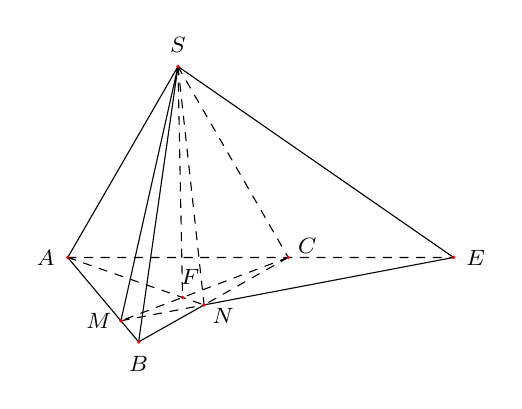
\begin{tikzpicture}[scale=0.7,font=\footnotesize,line join=round,line cap=round,>=stealth]
   \path
   (0,0) coordinate (A) 
   (4,0) coordinate (C) 
   (-50:2)  coordinate (B)
    (60:4) coordinate (S)
   (-50:1.5) coordinate  (M)
   (7,0)  coordinate (E);
  \coordinate (N) at (intersection  cs:first line={(M)--(E)},second line={(C)--(B)});
  \coordinate (F)  at (intersection cs:first line={(A)--(N)},second line={(C)--(M)});
   \draw (A)--(B)--(S)--cycle (S)--(M)
   (B)--(N) 
    (E)--(N)
    (S)--(E);
  \draw[dashed]  (A)--(E)
   (M)--(N) 
    (C)--(M)
   (A)--(N) 
   (S)--(F) 
   (S)--(N) 
   (C)--(N) 
    (S)--(C);
  \foreach \x/\g in {A/180,B/-90,C/30,S/90,M/180,N/-30,F/70,E/0}\fill[red]  (\x) circle (1pt)+(\g:4mm) node[black]{$\x$};
 \end{tikzpicture}
    }
   \itemch Sai. Trong mặt phẳng $(ABC)$, vẽ giao điểm $F$ của $AN$ và $MC$.\\ 
   Ta có $S$ và $F$ là hai điểm chung của hai mặt phẳng $(SAN)$ và  $(SCM)$.\\
   Suy ra $(SAN)\cap  (SCM)=SF$.
 \end{itemchoice}}
\end{ex}

% nguồn: Ok_dungsai_lop11_Lan1
\begin{ex}%[1H4N1-4]%[ma:4b845129]
 Cho tứ diện $S.ABC$. Gọi $M$  và $N$ lần lượt là hai điểm trên hai cạnh $AB$ và $BC$ sao cho $MN$ không song song với $AC$. Khi đó
 \choiceTF 
  {\True Đường thẳng $MN$ cắt đường  thẳng $AC$}
  {\True Giao điểm của đường thẳng  $MN$ và mặt phẳng $(SAC)$ là giao điểm của $MN$ và $AC$}
  {\True Giao tuyến của hai mặt  phẳng $(SMN)$ và $(SAC)$ đi qua giao điểm của $MN$ và $AC$}
  {Giao tuyến của hai mặt phẳng $(SAN)$ và $(SCM)$ đi qua giao điểm  của $MN$ và $AC$}
  \loigiai{
  \begin{center}
   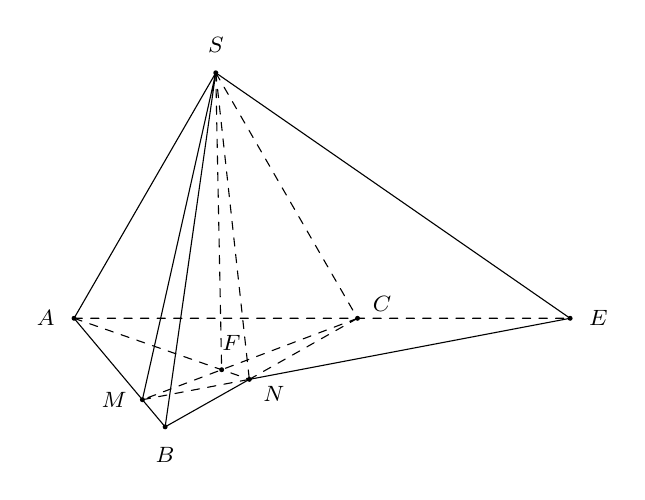
\begin{tikzpicture}[scale=0.9,font=\footnotesize,line join=round,line cap=round,>=stealth]
      \path
       (0,0) coordinate (A)
      (4,0) coordinate (C) 
      (-50:2) coordinate  (B)
      (60:4)  coordinate (S)
       (-50:1.5) coordinate (M)
       (7,0) coordinate (E);
     \coordinate (N)  at (intersection cs:first line={(M)--(E)},second line={(C)--(B)});
      \coordinate (F) at (intersection cs:first line={(A)--(N)},second line={(C)--(M)});
     \draw  (A)--(B)--(S)--cycle (S)--(M)
      (B)--(N) 
      (E)--(N) 
       (S)--(E);
     \draw[dashed]  (A)--(E)
       (M)--(N)
      (C)--(M) 
       (A)--(N)
      (S)--(F) 
      (S)--(N) 
       (C)--(N)
      (S)--(C); 
     \foreach \x/\g in  {A/180,B/-90,C/30,S/90,M/180,N/-30,F/70,E/0}\fill[black] (\x) circle (1pt)+(\g:4mm) node[black]{$\x$};
    \end{tikzpicture}
  \end{center}
  \begin{itemchoice}
   \itemch \textbf{Đúng}.\\  Vì $MN$ không song song và không trùng với $AC$ nên $MN$ cắt $AC$.
   \itemch \textbf{Đúng}.\\ Trong mặt phẳng $(ABC)$, vẽ giao điểm  $E$ của $MN$ và $AC$.\\
   Ta có $E\in AC$,  suy ra $E\in (SAC)$.\\
   Vậy $E$ là giao điểm của đường thẳng $MN$ và mặt phẳng  $(SAC)$.
   \itemch  \textbf{Đúng}.\\
   Ta có $S$ và $E$ là hai điểm chung của hai mặt phẳng $(SMN)$  và $(SAC)$.\\
   Suy  ra $(SMN)\cap (SAC)=SE$.
   \itemch \textbf{Sai}.\\ Trong mặt phẳng $(ABC)$, vẽ giao  điểm $F$ của $AN$ và $MC$.\\
   Ta có $S$ và $F$ là hai điểm  chung của hai mặt phẳng $(SAN)$ và $(SCM)$.\\
    Suy ra $(SAN)\cap (SCM)=SF$.
 \end{itemchoice}}
\end{ex}

% nguồn: Ok_dungsai_lop11_Lan1
\begin{ex}%[1H4H1-4]%[ma:adde8424]
 Cho tứ diện $ABCD$. Gọi $I$, $J$ lần lượt là trung điểm của $AD$, $BC$, $M$ là một điểm trên cạnh $AB$, $N$ là một điểm  trên cạnh $AC$. Khi đó
  \choiceTF
  {\True $IJ$ là giao  tuyến của hai mặt phẳng $(IBC)$, $(JAD)$}
  {\True $ND$ là giao tuyến của hai  mặt phẳng $(MND)$, $(ADC)$}
  {\True $BI$ là giao tuyến của hai mặt  phẳng $(BCI)$, $(ABD)$}
   {Giao tuyến của hai mặt phẳng $(IBC)$, $(DMN)$ song song với đường thẳng $IJ$}
  \loigiai{
  \begin{center}
   \begin{tikzpicture}[scale=1.1,font=\footnotesize,line join=round,line cap=round,>=stealth]
      \path
      (0,0) coordinate  (B)
      (1,-1.8)  coordinate (C)
      (4,0) coordinate  (D)
       (1.2,3.4) coordinate (A)
      ($(A)!0.5!(D)$) coordinate (I) 
      ($(C)!0.5!(B)$) coordinate  (J)
      ($(A)!0.4!(B)$)  coordinate (M)
      ($(A)!0.6!(C)$)  coordinate (N)
      (intersection of  B--I and M--D) coordinate (F)
      (intersection of I--C and N--D)  coordinate (E);
     \draw  (A)--(B)--(C)--(D)--cycle (J)--(A)--(C)--(I)
       (M)--(N)--(D);
     \draw[dashed] (I)--(B)--(D)--(J)--cycle  (D)--(M)
       (E)--(F);
     \foreach  \p/\q in {A/90,B/180,C/-90,D/0,M/140,N/50,I/60,J/230,F/90,E/30}
     \fill[black] (\p)  circle (1.0pt)
       ($(\p)+(\q:3mm)$) node{$\p$};
    \end{tikzpicture}
  \end{center}
  \begin{itemchoice}
    \itemch Ta có $I \in AD, AD \subset(JAD) \Rightarrow I \in(JAD) \Rightarrow IJ \subset(JAD)$.\\
   $J \in BC, BC \subset(IBC) \Rightarrow J  \in(IBC) \Rightarrow IJ \subset(IBC)$.\\
   Vậy $(IBC) \cap(JAD)=IJ$. 
   \itemch $ND$ là  giao tuyến của hai mặt phẳng $(MND),(ADC)$.
   \itemch $BI$ là giao tuyến của hai  mặt phẳng $(BCI),(ABD)$.
   \itemch Gọi $E=DN \cap  CI($ trong $m p(ACD))$ và $F=DM \cap BI$ (trong $(ABD)$).\\
   Ta  có $\heva{&E \in DN, DN \subset(DMN) \\
   & E\in IC, IC  \subset(IBC) }$\\
    $\Rightarrow E \in(DMN) \cap(IBC).\quad(1)$\\
   Tương tự: $\heva{&  F \in DM, DM \subset(DMN)\\
   & F \in BI, BI  \subset(IBC)} \Rightarrow F\in(DMN) \cap(IBC).\quad(2)$\\
   Từ $(1)$ và  $(2)$ suy ra $(DMN) \cap(IBC)=EF$.\\
   Khi đó $EF$ cắt $IJ$. 
  \end{itemchoice}
  }
\end{ex}

% nguồn: Ok_dungsai_lop11_Lan1
\begin{ex}%[1H4H1-4]%[ma:f31f5405]
 Cho bốn điểm $A$, $B$, $C$, $D$ không  đồng phẳng. Gọi $M$, $N$ lần lượt là trung điểm của $AC$ và $BC$. Trên đoạn $AD$ lấy điểm $P$ sao cho $BP=2PD$, gọi $E$ là giao điểm của $CD$ và $NP$. Khi đó các khẳng định sau đây đúng hay sai?
 \choiceTF 
  {\True $MN = (MNP)  \cap (ABC)$ }
  {\True $ME = (MNP) \cap (ACD)$} 
  {\True $E=CD\cap (MNP)$} 
  {\True $AD\cap  (MNP)= AD\cap ME$}
  \loigiai{
  \begin{center}
   \begin{tikzpicture}[scale=1,line join = round,line cap = round]
     \def\a{4} 
     \path (0:0) coordinate (B) 
      ++(0:\a) coordinate (D) 
      ++(-150:.8*\a) coordinate (C) 
      ($(B)+(70:\a)$) coordinate (A) 
       ($(A)!.5!(C)$) coordinate (M)
       ($(B)!.5!(C)$) coordinate (N)
      ($(B)!2/3!(D)$) coordinate  (P)
      ($(N)!3!(P)$) coordinate (I) 
      ($(C)!3!(D)$) coordinate (K) 
      (intersection of  N--I and C--K) coordinate (E)
      (intersection of A--D  and M--E) coordinate (F);
      \draw[dashed] (B)--(D)
       (N)--(E)
      (M)--(P); 
     \draw  (B)--(A)--(D)
       (A)--(C)
      (B)--(C)--(D) 
       (M)--(E)--(D)
       (M)--(N);
     \foreach \x/\g  in {A/90,B/180,C/-45,D/-60,M/150,N/-150,P/90,E/90,F/80}
     \fill[black] (\x) circle (1pt) 
      ($(\g:3mm)+(\x)$) node  {$\x$};
    \end{tikzpicture}
  \end{center}
  \begin{itemchoice}
   \itemch {\bf Đúng.}  \\
   Vì $\heva{&M\in AC\\& N\in BC }\Rightarrow MN \subset (ABC)$ và $MN\subset (MNP)$ nên  $MN = (MNP) \cap (ABC)$.
   \itemch  {\bf Đúng.}\\
   Vì $\heva{&M\in AC\\& E\in CD }\Rightarrow ME \subset (ACD)$ và $\heva{&M\in MN\\& E\in NP }\Rightarrow ME  \subset (MNP)$\\
   nên  $ME = (MNP) \cap (ACD)$.
   \itemch  {\bf Đúng.}\\
   Vì $\heva{&ME \subset (MNP) \Rightarrow E \in (MNP)\\& E\in  DC}$ nên $ E=CD\cap (MNP)$.
    \itemch {\bf Đúng.}\\
   Vì $ME$ và $CD$ cùng nằm trong mặt phẳng $(ACD)$ và không song song nên cắt nhau. Gọi $F$ là giao điểm  của $AD$ và $ME$.\\
   Vì $F\in ME \subset (MNP)$ nên  $F= AD\cap (MNP)$.\\
   Vậy $AD\cap  (MNP)= AD\cap ME =F$.
  \end{itemchoice}
  }
\end{ex}

% nguồn: Ok_dungsai_lop11_Lan1
\begin{ex}%[1H4H1-4]%[ma:d340d101]
  \immini{
 Cho hình chóp $S.ABC$. Gọi $E$, $F$ lần lượt là trung điểm của $SA$, $SC$  và $G$ là trọng tâm tam giác $ABC$. Xét tính đúng sai của các khẳng định sau
  \choiceTF
  {\True $\left(BEF\right) \cap \left(ABC\right)=d$ đi qua $B$ và song  song với $AC$}
  { \True $\left(GEF\right) \cap \left(ABC\right)=d$ đi  qua $G$ và song song với $AC$}
  {$\left(BEF\right) \cap \left(ABC\right)=d$ đi qua $B$ và song song với $AB$} 
  {$\left(GEF\right)  \cap \left(ABC\right)=d$ đi qua $G$ và song song với $BC$}
   }{
  \begin{tikzpicture}[scale=0.9,line join=round,line cap=round]
    \coordinate (S)  at (1,3);
     \coordinate (A) at (0,0);
    \coordinate (B)  at (2,-2);
    \coordinate (C) at (4.5,0); 
    \coordinate (E) at ($(A)!0.5!(S)$); 
    \coordinate (F) at  ($(S)!0.5!(C)$);
    \coordinate (I) at ($(A)!0.5!(B)$); 
     \coordinate (G) at ($(C)!2/3!(I)$);
    \draw  (S) node[above]{$S$}--(A) node[left]{$A$}--(B) node[below]{$B$}--(C) node[right]{$C$}--(S)--(B);
    \draw[dashed] (C)--(A) 
     (E)--(G) 
     (F)--(G)  node[below]{$G$}
     (C)--(I) node[left]{$I$} 
     (E) node[left]{$E$}--(F) node[above  right]{$F$};
     \foreach \point in {A,B,C,E,F,G,I}
    \fill [black] (\point) circle  (1pt);
   \end{tikzpicture}
   }
  \loigiai{
  \begin{itemchoice}
   \itemch Xét hai mặt phẳng $\left(BEF\right)$ và $ \left(ABC\right)$ ta có  $B \in \left(BEF\right) \cap \left(ABC\right)$\\
   lại có 
   $\heva{&EF \subset \left(BEF\right) \\ &AC  \subset \left(ABC\right) \\& EF \parallel AC}$ \\
   nên $\left(BEF\right) \cap \left(ABC\right)=d$ đi qua $B$ và song song với  $AC$
   \itemch Xét hai mặt phẳng $\left(GEF\right)$ và $ \left(ABC\right)$ ta  có $G \in \left(GEF\right) \cap \left(ABC\right)$\\
   lại  có
   $\heva{&EF \subset \left(BEF\right) \\ &AC \subset  \left(ABC\right) \\& EF \parallel AC}$ \\
   nên $\left(BEF\right) \cap \left(ABC\right)=d$ đi qua $G$ và song song với  $AC$
   \itemch Xét hai mặt phẳng $\left(BEF\right)$ và  $ \left(ABC\right)$ ta có $B \in \left(BEF\right) \cap \left(ABC\right)$\\
   lại  có
   $\heva{&EF \subset \left(BEF\right) \\ &AC  \subset \left(ABC\right) \\& EF \parallel AC}$ \\
   nên $\left(BEF\right)  \cap \left(ABC\right)=d$ đi qua $B$ và song song với $AC$
   \itemch Xét hai mặt phẳng $\left(GEF\right)$ và $ \left(ABC\right)$ ta có $G  \in \left(GEF\right) \cap \left(ABC\right)$\\
   lại  có
   $\heva{&EF \subset  \left(BEF\right) \\ &AC \subset \left(ABC\right) \\& EF \parallel AC}$ \\
   nên $\left(BEF\right)  \cap \left(ABC\right)=d$ đi qua $G$ và song song với $AC$
  \end{itemchoice}
 } 
\end{ex}

% nguồn: Ok_dungsai_lop11_Lan1
\begin{ex}%[1H4H1-4]%[ma:8bd554e1]
 Cho hình  chóp $S.ABCD$ có đáy là hình bình hành. Gọi $M$ là trung điểm của $SC$. Gọi $I$ là giao điểm của đường thẳng $AM$ và mặt phẳng $(SBD)$. Khi đó
  \choiceTF
  {\True $AM\cap  SO=I$}
   {$IA=3IM$}
  {\True Giao điểm  $E$ của đường thẳng $SD$ và mặt phẳng $(ABM)$ là điểm thuộc đường thẳng $BI$}
  {\True Gọi $N$ là một điểm tuỳ ý trên cạnh $AB$. Khi đó giao điểm của đường thẳng $MN$ và mặt phẳng $(SBD)$ là điểm thuộc giao tuyến của hai  mặt phẳng $(SBD)$, $(SNC)$}
 \loigiai{ 
  \begin{itemchoice}
   \itemch Đúng. Trong $(SAC)$ có $AM\cap SO=I$. 
   \itemch Sai. Ta có $\heva{& I\in AM \\ &  I\in SO\subset (SBD)} \Rightarrow I\in AM\cap (SBD)$.\\
   Tam giác $SAC$ có hai đường trung tuyến $AM$ và $SO$ cắt nhau tại $I$, suy ra $I$ là trọng tâm của tam giác $SAC$.  Từ đó ta có $IA=2IM$.
   \itemch Đúng. \immini 
    {
   Trong  $(SBD)$ có $BI\cap SD=E$.\\
   Ta có $\heva{&  E\in SD \\ & E\in BI\subset (ABM)} \Rightarrow I\in SD\cap (ABM)$.
    }
    {
   \begin{tikzpicture}[line cap=round,line join=round,>=stealth,scale=0.75]
     \def \a{-1.5}  \def \b{-1.5} \def \c{4} \def \h{5}
     \path (0,0)  coordinate (D)
      +(\a,\b)  coordinate (A)
      +(\c,0)  coordinate (C)
       ($(A)+(C)-(D)$) coordinate (B)
      ($(A)!1/2!(B)$) coordinate (H) 
       +(0,\h) coordinate (S)
      ($(B)!1/2!(D)$)  coordinate (O)
      ($(S)!1/2!(C)$)  coordinate (M)
       ($(S)!1/2!(D)$) coordinate (E)
      ($(S)!2/3!(O)$)  coordinate (I);
     \draw  [dashed,teal] (A)--(D)--(C)
       (D)--(S)
      (A)--(C) 
       (B)--(D)
       (A)--(M)
       (B)--(E)
       (S)--(O);
     \draw  [teal](S)--(A)--(B)--(C)--(S)--(B)
      (B)--(M); 
     \foreach  \x/\g in {A/180,B/0,C/0,D/180,S/90,E/180,I/180,M/30,O/-90}\fill[draw,fill=white] (\x) circle (1pt)+(\g:4mm) node[black]{$\x$};
    \end{tikzpicture}
    }
   \itemch Dúng.  \immini {Trong $(ABCD)$ có $CN\cap BD=F$.\\
   Trong $(SNC)$ có  $SF\cap MN=J$.\\
   Ta có $\heva{& J\in MN \\  & J\in SF\subset (SBD)} \Rightarrow J\in MN\cap (SBD)$.}
   {\begin{tikzpicture}[line cap=round,line join=round,>=stealth,scale=0.75]
  \def \a{-1.5} \def \b{-1.5}  \def \c{4} \def \h{5}
   \path (0,0) coordinate (D)
    +(\a,\b) coordinate (A)
   +(\c,0)  coordinate (C)
    ($(A)+(C)-(D)$) coordinate (B)
   ($(A)!1/2!(B)$) coordinate  (H)
   +(0,\h) coordinate  (S)
   ($(B)!1/2!(D)$)  coordinate (O)
   ($(S)!1/2!(C)$) coordinate (M) 
    ($(A)!1/4!(B)$) coordinate (N)
   ($(B)!3/7!(D)$) coordinate  (F);
  \draw [dashed,teal] (A)--(D)--(C) 
   (D)--(S) 
   (N)--(C) 
    (B)--(D)
    (N)--(M)
   (B)--(E) 
    (S)--(F);
   \draw [teal](S)--(A)--(B)--(C)--(S)--(B)
   (S)--(N); 
  \coordinate (J)  at (intersection cs:first line={(M)--(N)},second line={(S)--(F)});
  \foreach \x/\g  in {A/180,B/0,C/0,D/180,S/90,F/-90,M/30,N/-90,J/0}\fill[draw,fill=white] (\x) circle (1pt)+(\g:4mm) node[black]{$\x$};
 \end{tikzpicture}
   } 
 \end{itemchoice}}
\end{ex}

% nguồn: Ok_dungsai_lop11_Lan2
\begin{ex}%[1H4H1-4]%[ma:6e034577]
	Cho hình chóp $S.ABCD$ có đáy là hình bình hành. Gọi $M$ là trung điểm của $SC$. Gọi $I$ là giao điểm của đường thẳng $AM$ và mặt phẳng $(SBD)$. Khi  đó
	\choiceTF 
		 {\True $AM\cap SO=I$}
		{$IA=3IM$} 
		{\True Giao điểm $E$ của  đường thẳng $SD$ và mặt phẳng $(ABM)$ là điểm thuộc đường thẳng $BI$}
		{\True Gọi $N$  là một điểm tuỳ ý trên cạnh $AB$. Khi đó giao điểm của đường thẳng $MN$ và mặt phẳng $(SBD)$ là một điểm thuộc $(SNC)$}
	\loigiai{ 
		\begin{center}
			\begin{tikzpicture}[scale=0.8,font=\footnotesize,line join=round,line cap=round,>=stealth]
					\path 
						(0,0) coordinate (D) 
						(7,0) coordinate (C) 
						 (6,-2) coordinate (B)
						(-1,-2) coordinate  (A)
						(-0.8,5)  coordinate (S)
						 (8,0) coordinate (Z)
						($(A)!0.5!(C)$) coordinate  (O)
						($(C)!0.5!(S)$) coordinate  (M);
					\path [name  path =am] (A)--(M);
					\path [name path  =so] (S)--(O);
					\path [name intersections ={of  =am and so,by={I}}];
					\path [name path =be]  (I)--($(I)!1!180:(B)$);
					\path  [name path =sd] (S)--(D);
					\path [name intersections ={of =be  and sd,by={E}}];
					 \path (C)--(Z);
					\draw (S)--(A)--(B)--(C)--(S)--(B)--(M); 
					\draw[dashed]  (A)--(D)--(C)--(A)--(M)
						 (E)--(B)--(D)--(S)--(O);
					\foreach \i/\g in  {A/180,B/0,C/0,D/180,S/90,E/45,I/-100,M/45,O/-90}
					\fill (\i) circle  (1pt)+(\g:3mm) node[scale=1]{$\i$};
				\end{tikzpicture}
			\begin{tikzpicture}[scale=0.7,font=\footnotesize,line join=round,line cap=round,>=stealth]
					 \path
						(0,0)  coordinate (D)
						 (7,0) coordinate (C)
						(5,-2) coordinate  (B)
						(-2,-2) coordinate  (A)
						(-0.3,5)  coordinate (S)
						($(C)!0.5!(S)$) coordinate  (M)
						 ($(A)!0.4!(B)$) coordinate (N);
					\path [name path =cn] (C)--(N); 
					\path [name  path =bd] (B)--(D);
					\path [name intersections ={of =cn and  bd,by={F}}];
					\path  [name path =sf] (S)--(F);
					\path [name  path =mn] (M)--(N);
					\path [name intersections ={of =mn  and sf,by={J}}];
					\draw (S)--(A)--(B)--(C)--(S)--(B) 
						(S)--(N); 
					\draw[dashed] (A)--(D)--(C)--(N) 
						(B)--(D)--(S)--(F) 
						(N)--(M); 
					\foreach \i/\g in {A/180,B/0,C/0,D/180,S/90,F/-90,J/0,M/45,N/-90} 
					\fill[black] (\i)  circle (1pt)+(\g:3mm) node[scale=1]{$\i$};
				\end{tikzpicture}
		\end{center}
		\begin{itemchoice}
			\itemch Có $O\in AC \subset (SAC)$, $M\in SC \subset  (SAC)$. Trong $(SAC)$ có $AM\cap SO=I$.
			\itemch Ta có $\heva{&I\in AM\\&I\in SO\subset(SBD)}$ suy ra  $I\in AM\cap(SBD)$.\\
			Tam giác $SAC$ có  hai đường trung tuyến $AM$ và $SO$ cắt nhau tại $I$, suy ra $I$ là trọng tâm của tam giác $SAC$. Từ đó ta có $IA=2IM$.
			\itemch Trong $(SDB)$  gọi $E=BI\cap SD$.\\
			Ta có $\heva{&E\in SD\\&E\in IB\subset(ABM)}$ nên $I\in  SD\cap(ABM)$.
			\itemch Trong $(ABCD)$ gọi  $F=CN\cap BD$.\\
			Trong $(SNC)$ gọi $J=SF\cap  MN$.\\
			Ta có \[\heva{&J\in MN\\&J\in  SF\subset(SBD)}\Rightarrow J\in MN\cap(SBD).\]
		\end{itemchoice}
	} 
\end{ex}

% nguồn: Ok_dungsai_lop11_Lan2
\begin{ex}%[1H4H1-4]%[ma:676bf799]
	Cho hình chóp $S.ABCD$ với $M$ là  một điểm trên cạnh $SC$, $N$ là một điểm trên cạnh $BC$. Gọi $O=AC\cap BD$ và $K=AN\cap CD$. Khi đó
	\choiceTF 
		{\True $SO$ là giao tuyến  của hai mặt phẳng $(SAC)$ và $(SBD)$}
		{\True Giao điểm của đường thẳng $AM$ và mặt phẳng $(SBD)$ là điểm nằm trên cạnh  $SO$}
		{\True $KM$ là giao  tuyến của hai mặt phẳng $(AMN)$ và $(SCD)$}
		{\True Giao điểm của đường thẳng $SD$ và mặt  phẳng $(AMN)$ là điểm nằm trên cạnh $KM$}
	 \loigiai{
		\begin{center}
			\begin{tikzpicture}[scale=1,font=\footnotesize,line join=round,line cap=round,>=stealth]
					 \path
						(0,0) coordinate  (D)
						(7,0)  coordinate (A)
						(5,-3.5)  coordinate (B)
						(1.5,-2.5)  coordinate (C)
						 (3.5,3) coordinate (S)
						($(S)!0.45!(C)$) coordinate  (M)
						($(C)!0.6!(B)$) coordinate (N); 
					\path [name path  =bd] (B)--(D);
					\path [name path =ac]  (A)--(C);
					\path [name intersections  ={of =bd and ac,by={O}}];
					\path  [name path =dk] (C)--($(C)!1!180:(D)$);
					\path  [name path =ak] (N)--($(N)!0.4!180:(A)$);
					\path [name intersections ={of  =dk and ak,by={K}}];
					 \path [name path =hk] (M)--($(M)!0.4!180:(K)$);
					\path  [name path =sd] (S)--(D);
					\path [name intersections ={of =hk  and sd,by={H}}];
					\path  [name path =so] (S)--(O);
					\path [name path  =am] (A)--(M);
					\path [name intersections ={of =so and am,by={P}}]; 
					 \draw (S)--(D)--(K)--(N)--(B)--(A)--(S)--(B)
						 (N)--(M)--(C)
						(H)--(M)--(S) 
						(M)--(K); 
					 \draw[dashed] (M)--(A)--(D)--(B)
						 (N)--(C)--(A)--(N)
						(S)--(O); 
					 \foreach \i/\g in {A/0,B/-90,C/180,D/180,S/90,H/135,K/-90,M/135,N/-90,O/-90,P/45}
					\fill (\i) circle  (1pt)+(\g:3mm) node[scale=1]{$\i$};
				\end{tikzpicture}
		\end{center}
		\begin{itemchoice}
			\itemch Tìm giao tuyến của hai mặt phẳng  $(SAC)$ và $(SBD)$.\\
			Dễ thấy $S$ là điểm chung của hai mặt phẳng $(SAC)$  và $(SBD)$.\\
			Trong mặt  phẳng $(ABCD)$, gọi $O=AC\cap BD$.\\
			Vì $\heva{&O\in AC,\ AC\subset(SAC)\\&O\in BD,\  BD\subset(SBD)}$ nên $O\in(SAC)\cap(SBD)$.\\
			Vậy  $SO=(SAC)\cap(SBD)$.
			\itemch Tìm giao điểm của $AM$  và mặt phẳng $(SBD)$.\\
			Trong mặt phẳng $(SAC)$, gọi  $P=AM\cap SO$.\\
			 Ta có
			\[\heva{&P\in AM\\&P\in  SO,\ SO\subset(SBD)}\Rightarrow P=AM\cap(SBD).\]
			\itemch Xét  mặt phẳng phụ $(SCD)$ chứa $SD$. Ta tìm giao tuyến của hai mặt phẳng $(AMN)$ và $(SCD)$.\\
			Trong mặt phẳng $(ABCD)$, gọi $K=AN\cap  CD$.\\
			Khi  đó
			\[\heva{&K\in AN,\  AN\subset(AMN)\\&K\in CD,\ CD\subset(SCD)}\Rightarrow K\in(AMN)\cap(SCD).\]
			Mặt  khác $M\in SC$, $SC\subset(SCD)$ nên $M\in(SCD)$, suy ra $M\in(SCD)\cap(AMN)$.\\
			Vậy  $KM=(SCD)\cap(AMN)$.
			 \itemch Trong mặt phẳng $(SCD)$ gọi $H=KM\cap SD$.\\
			 Ta có
			\[\heva{&H\in SD\\&H\in KM,\  KM\subset(AMN)}\Rightarrow H=SD\cap(AMN).\]
		\end{itemchoice}
	 }
\end{ex}

% nguồn: Ok_dungsai_lop11_Lan1
\begin{ex}%[1H4V1-4]%[ma:09975988]
 Cho tứ giác $ABCD$ có $AC$ và $BD$ cắt nhau tại $O$ và  một điểm $S$ không thuộc mặt phẳng $(ABCD)$. Trên đoạn $SC$ lấy một điểm $M$ không trùng với $S$ và $C$, $K=AM\cap SO$. Xét tính đúng sai của các phát biểu sau
 \choiceTF 
  {$SO$ là giao tuyến của  hai mặt phẳng $(SAC)$ và $(ABC)$}
   {\True $SO$ là giao tuyến của hai mặt phẳng $(SAC)$ và $(SBD)$}
  {\True Giao điểm của $SO$  và mặt phẳng $(ABM)$ là điểm $K$}
  {Giao điểm của $SD$  với mặt phẳng $(ABM)$ là điểm $N$ thuộc đường thẳng $AK$}
  \loigiai{
  \begin{itemchoice}
   \itemch $AC$ là giao tuyến của hai mặt phẳng  $(SAC)$ và $(ABC)$.
    \itemch $SO$ là giao tuyến của hai mặt phẳng $(SAC)$ và $(SBD)$.
   \itemch Trong mặt phẳng  $(SAC)$, gọi $K=AM\cap SO$.\\
   Vì  $\heva{&K\in AM, AM\subset (ABM)\\&K\in SO}\Rightarrow K=SO\cap (ABM)$.
   \itemch Ta có $B\in  (SBD)\cap (ABM)$.\\
   Ta  có $\heva{&K\in AM, AM\subset (ABM)\\&K\in SO, SO\subset (SBD)}\Rightarrow K\in (SBD)\cap (ABM)$.\\
   Do đó $BK=(SBD)\cap (ABM)$.\\ 
   Trong mặt  phẳng $(SBD)$ gọi $N=BK\cap SD$.\\
   Ta có $\heva{&N\in SD\\&N\in  BK, BK\subset (ABM)}\Rightarrow N=SD\cap (ABM)$.
  \end{itemchoice}
  }
\end{ex}

% nguồn: Ok_dungsai_lop11_Lan2
\begin{ex}%[1H4V1-4]%[ma:2f07c511]
	Cho hình chóp  $S.ABCD$ có đáy là hình bình hành, $AC$ và $BD$ cắt nhau tại $O$. Gọi $I$ là trung điểm $SO$. Mặt phẳng $(ICD)$ cắt $SA$, $SB$ lần lượt tại $M$, $N$. Khi đó:
	 \choiceTF
		{\True Điểm $M$ là giao điểm của đường  thẳng $SA$ với mặt phẳng $(ICD)$}
		{Ta có $SN=\dfrac{2}{3}SB$} 
		{Cho ${AB=a}$ thì $MN=\dfrac{a}{2}$} 
		{Trong mặt phẳng $(CDMN)$, gọi $K$ là giao điểm của $CN$ và $DM$. Khi  đó $SK$ và $BC$ chéo nhau}
	 \loigiai{
		- Xác  định $M, N$:\\
		Trong mặt phẳng $(SAC)$, kẻ $CI$ cắt  $SA$ tại $M$;\\
		Trong mặt phẳng  $(SBD)$, kẻ $DI$ cắt $SB$ tại $N$.\\
		 Vì $\heva{
		&M\in  CI,CI\subset (ICD) \\
		&M\in SA } $  $\Rightarrow M=SA\cap (ICD)$.\\
		 Tương tự: $\heva{
		&N\in DI,DI\subset (ICD)  \\
		&N\in SB  } $ $\Rightarrow N=SB\cap (ICD)$.\\
		-Tính $MN$ theo  $a$\\
		Gọi $E$ là trung điểm $BN, OE$ là đường trung bình của tam  giác $BDN$ $\Rightarrow OE\parallel DN$.\\
		Trong tam giác $SOE$,  ta có $NI$ qua trung điểm $I$ của $SO$ và $NI\parallel OE$, $N$ là trung điểm của $SE$.\\
		\centerline{ 
		\begin{tikzpicture}[font=\scriptsize,blue]
				 \def\a{4}
				\path 
					 (0:0) coordinate (A)
					(210:3) coordinate  (B)
					++(0:5)  coordinate (C)
					($(A)+(C)-(B)$) coordinate (D) 
					(intersection of A--C and B--D) coordinate  (O)
					 ($(O)+(90:4)$) coordinate (S)
					($(S)!1/2!(O)$) coordinate  (I)
					(intersection of I--C and  S--A) coordinate (M)
					(intersection of  I--D and S--B) coordinate (N)
					($(N)!1/2!(B)$)  coordinate (E)
					(intersection of N--C and  M--D) coordinate (K)
					($(O)!.75!(N)$)  coordinate (F);
				\draw[dashed,thin,black] (A)--(B)--(D)--cycle  (C)--(A)--(S)--(O)--(E)
					(C)--(M)--(N)--(D)--(K); 
				\draw[]  (B)--(C)--(D)
					 (B)--(S)
					(C)--(S) 
					(D)--(S) 
					 (C)--(K)--(S);
				\foreach  \x/\y in {A/135,B/-135,C/-45,D/45,S/90,O/-90,I/210,M/25,N/180,E/180,K/180}
				 \fill[black] (\x) circle (1pt)
					($(\y:2.5mm)+(\x)$)  node {$\x$};
			\end{tikzpicture}
		} 
		- Vậy $SN=NE=EB$ hay $SN=\dfrac{1}{3}  SB$.\\
		 Hoàn toàn tương tự, ta chứng minh được $SM=\dfrac{1}{3} SA$.\\
		Khi đó hai tam giác $SMN$, $SAB$ đồng dạng vì có góc $S$ chung  và $\dfrac{SM}{SA} =\dfrac{SN}{SB}=\dfrac{1}{3}$.\\
		Xét tam giác $SAB$, theo định lí Thalès, ta  có:\\
		$\dfrac{MN}{AB}=\dfrac{SM}{SA} =\dfrac{1}{3} \Rightarrow MN=\dfrac{AB}{3}  =\dfrac{a}{3} $.\\
		Chứng minh $SK\parallel  BC\parallel AD$:\\
		Dễ thấy $S$  là điểm chung của hai mặt phẳng $(SBC)$ và $(SAD)$.\\
		 Ta có $\heva{
		&K \in  CN, CN \subset(SBC) \\
		&K \in DM, DM \subset(SAD) } $. $\Rightarrow K \in(S  B C) \cap(S A D)$\\
		Vì vậy $SK=(SBC)\cap(SAD)$.\\ 
		 Khi đó $\heva{
		 &SK=(SBC)\cap (SAD) \\
		 &BC\subset (SBC),AD\subset (SAD) \\
		&BC\parallel AD  }$ $\Rightarrow SK\parallel BC\parallel AD$
		\begin{itemchoice}
			\itemch  Đúng.
			\itemch  Sai.
			 \itemch Sai.
			 \itemch Sai.
		\end{itemchoice}
	} 
\end{ex}

% nguồn: Ok_dungsai_lop11_Lan2
\begin{ex}%[1H4V1-4]%[1H4V1-6]%[ma:237f6ddb]
	Cho hình chóp  $S.ABCD$ có đáy $ABCD$ là hình thang ($AD$ là đáy lớn, $BC$ là đáy nhỏ). Gọi $E$, $F$ lần lượt là trung điểm của $SA$ và $SD$, $K$ là giao điểm của các đường thẳng $AB$ và $CD$. Khi đó:
	\choiceTF 
		{\True Giao điểm $M$ của  đường thẳng $SB$ và mặt phẳng $(CDE)$ là điểm thuộc đường thẳng $KE$}
		{Đường thẳng $SC$ cắt mặt phẳng $(EFM)$ tại $N$. Tứ giác $EFNM$  là hình bình hành}
		{\True Các đường thẳng $AM$, $DN$, $SK$  cùng đi qua một điểm}
		{Cho biết $AD=2 BC$. Tỉ số diện tích  của hai tam giác $KMN$ và $KEF$ bằng $\dfrac{S_{\triangle KMN}}{S_{\triangle KEF}} =\dfrac{2}{3}$}
	\loigiai{ 
		\begin{center}
			\begin{tikzpicture}[font=\scriptsize,blue]
					\path 
						(0:0) coordinate (A) 
						 (0:4) coordinate (D)
						(75:4) coordinate  (S)
						(-60:2.5) coordinate (K) 
						(barycentric  cs:A=1,K=1) coordinate (B)
						(barycentric  cs:D=1,K=1) coordinate (C)
						(barycentric  cs:A=1,S=1) coordinate (E)
						(barycentric cs:D=1,S=1) coordinate (F) 
						(barycentric cs:S=1,K=1) coordinate (I) 
						(barycentric cs:A=1,K=1,S=1) coordinate (M) 
						(barycentric  cs:D=1,K=1,S=1) coordinate (N);
					\draw[dashed,thin,black] (A)--(D) 
						(B)--(C)--(E)--(D) 
						 (E)--(F)--(M)--(N);
					\draw[]  (S)--(A)--(K)--(D)--(S)--(K)
						 (E)--(K)--(F)
						(A)--(I)--(D) 
						 (B)--(S)--(C);
					\foreach \x/\y in  {A/180,D/0,S/90,K/-90,B/210,C/-30,I/-60,M/150,N/30,E/150,F/30}
					\fill[black] (\x) circle (1pt) 
						($(\y:3mm)+(\x)$)  node {$\x$};
				\end{tikzpicture}
		\end{center}
		\begin{itemchoice}
			\itemch  Đúng.\\
			 Có $SK=(SAB)\cap(SCD)$.\\
			Trong mp$(SAB)$, gọi $M=KE\cap  SB$, có $KE\subset(CDE)$.\\
			Do đó  $SB\cap(CDE)=M$.
			\itemch Sai.\\ 
			Trong mp$(SCD)$, gọi  $N=KF\cap SC$, có $KF\subset(EFM)$.\\
			 Do đó $SC\cap(EFM)=N$.\\
			Có $\Rightarrow  \heva{
			&MN=(EFK)\cap (SBC)  \\
			&EF\parallel  BC;\, EF\subset (EFK),\, BC\subset (SBC) \\
			}$ $\Rightarrow MN\parallel  EF\parallel BC$.\\
			Suy ra tứ giác  $EFNM$ là hình thang.
			\itemch  Đúng.\\
			Trong mp$(ADNM)$, gọi $I=AM  \cap DN$.\\
			Mà $\heva{ 
			&I\in AM,AM\subset (SAB)  \\
			&I\in  CD,CD\subset (SCD) }$ $\Rightarrow I\in (SAB)\cap (SCD)$,\\
			Hay $I \in S  K$.\\
			 Kết luận 3 đường thẳng $AM, DN, SK$ đồng quy tại điểm $I$.
			\itemch Sai.\\ 
			Khi $AD=2BC$ dễ dàng chứng minh được $B, C$ lần lượt là trung điểm của $KA$  và $KD$.\\
			Suy ra $M, N$ lần lượt là trọng tâm của hai tam giác  $SAK$ và $SDK$.\\
			Do đó $MN=\dfrac{2}{3}{EF}$,  gọi $h_1, h_2$ lần lượt là độ dài đường cao xuất phát từ đỉnh $K$ xuống hai đáy $MN$ và $EF$, dễ thấy $h_1=\dfrac{2}{3} h_2$.\\
			Vậy $\dfrac{S_{\Delta K M N}}{S_{\Delta K E F}}=\dfrac{\tfrac{1}{2} MN  \cdot h_1}{\frac{1}{2} EF \cdot h_2}=\dfrac{\tfrac{2}{3} EF \cdot \tfrac{2}{3} h_2}{EF \cdot h_2}=\dfrac{4}{9}$.
		\end{itemchoice}
	 }
\end{ex}


%%%%%%%%%%%%%%%% TRẢ LỜI NGẮN %%%%%%%%%%%%%%%%

% nguồn: Ok_TraLoiNgan_Lop11_Lan1
\begin{ex}%[1H4N1-4]%[ma:fdebd085]
	Cho tứ diện $ABCD$. Gọi $I$ là trung điểm $AB$, $J$ là điểm thuộc cạnh $AD$ sao cho $JD=\dfrac{1}{3}JA$, gọi $E=IJ\cap BD$. Tìm giao điểm của đường thẳng $IJ$ và mp $(BCD)$. Nếu giao điểm thuộc $(ABD)$ chọn $1$, thuộc $(ACD)$ chọn $2$, thuộc $(ABD)$ chọn $3$, thuộc cạnh $AC$ chọn $4$, không nằm ở trường hợp nào của các lựa  chọn trước thì chọn $5$.
	 \shortans{3}
	 \loigiai{
	 \immini
		{Trong mặt phẳng $(ABD)$, gọi  $ E=IJ\cap BD$.\\
		Ta có $\heva{& E\in IJ \\ & E\in BD\subset (BCD)} \Rightarrow  E=IJ\cap (BCD)$.
		 }
		{\begin{tikzpicture}[line join = round,line cap = round,>=stealth,font=\footnotesize,scale=0.7]
		\path (0,0) coordinate  (B)
			(2,3) coordinate (A) 
			(-70:2)  coordinate (C)
			(4,0) coordinate  (D)
			($(A)!1/2!(B)$) coordinate (I) 
			($(A)!3/4!(D)$)  coordinate (J);
		\coordinate (E) at (intersection cs:first line={(I)--(J)},second line={(B)--(D)}); 
		\draw  [dashed] (B)--(D)
			(I)--(J); 
		\draw  (A)--(B)--(C)--(D)--(E)--(J)--(A)--(C)
			(J)--(D); 
		\foreach \x/\g in  {B/180,A/90,C/180,D/-45,J/45,E/0,I/180}\draw[fill=white] (\x) circle (1pt)+(\g:4mm) node{$\x$};
	\end{tikzpicture}
		 }
	} 
\end{ex}

% nguồn: Ok_TraLoiNgan_Lop11_Lan2
\begin{ex}%[1H4H1-4]%[ma:de8c1d27]
	\immini[thm]{Cho hình chóp $S.ABCD$ có đáy là hình bình hành như hình vẽ. Gọi $N$ là trung điểm $SC$, $H$ là giao điểm của đường thẳng $AN$ và mặt phẳng $(SBD)$. Biết $AH=k\cdot HN$, tìm $k$?}{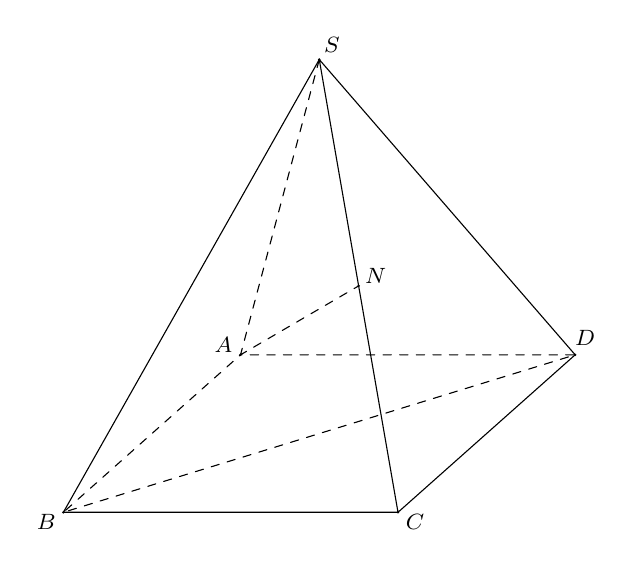
\begin{tikzpicture}[font=\footnotesize,line join=round,line cap=round,>=stealth,scale=0.5]
		\path 
			(0,0) coordinate (A) 
			(-4.5,-4) coordinate  (B)
			 (4,-4) coordinate (C)
			(8.5,0)  coordinate (D)
			(2,7.5)  coordinate (S)
			(3,1.75) coordinate  (N);
		\draw  (S)--(C)
			 (S)--(B)
			(D)--(S)--(B)--(C)--(D); 
		 \draw[dashed] (S)--(A)--(B)--(D)--(A)--(N);
		\foreach \x/\pos  in{A/150,B/-150,C/-30,D/60,S/50,N/30}
		\fill  (\x) circle (1pt) node[{shift=(\pos:0.25)}]{$\x$};
	\end{tikzpicture}
	 }
	 \shortans{2}
	\loigiai{\begin{center}
		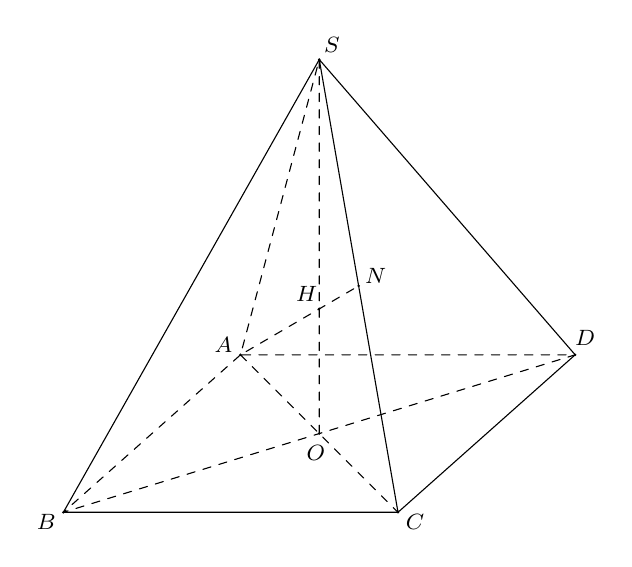
\begin{tikzpicture}[font=\footnotesize,line join=round,line cap=round,>=stealth,scale=0.5]
				 \path
					(0,0) coordinate (A) 
					(-4.5,-4)  coordinate (B)
					 (4,-4) coordinate (C)
					(8.5,0) coordinate (D) 
					(2,7.5) coordinate  (S)
					 (3,1.75) coordinate (N)
					(2,-2)  coordinate (O)
					(2,1.17)  coordinate (H);
				 \draw (S)--(C)
					(S)--(B) 
					 (D)--(S)--(B)--(C)--(D);
				\draw[dashed]  (O)--(S)--(A)--(B)--(D)--(A)--(N)
					(A)--(C); 
				\foreach \x/\pos in{A/150,B/-150,C/-30,D/60,S/50,N/30,O/-100,H/130} 
				\fill (\x) circle (1pt)  node[{shift=(\pos:0.25)}]{$\x$};
			\end{tikzpicture}
	\end{center}
	Gọi  $O=AC \cap BD$.\\
	Trong $(SAC)$, gọi $H=SO \cap AN$. Mà $SO \subset(SBD)$.\\ 
	Do đó  đó $H=AN \cap(SBD)$.\\
	Xét tam giác $SAC$ có $O$, $N$ lần lượt là  trung điểm của $AC$, $SC$.\\
	Suy ra $AN$, $SO$ là hai đường trung tuyến của tam giác $SAC$.\\ 
	Mà $H=SO \cap AN$.\\ 
	Suy ra $H$ là trọng tâm của tam giác  $SAC$. Suy ra $AH=2HN$.\\
	Vậy $k=2$. 
} 
\end{ex}

% nguồn: Ok_TraLoiNgan_Lop11_Lan2
\begin{ex}%[1H4H1-4]%[ma:bcd0f2a3]
	Cho hình chóp $S.ABCD$ có đáy là hình bình hành.$M$ là trung điểm của $SC$. Gọi $I$ là giao điểm của đường thẳng $AM$  với mặt phẳng $(SBD)$. Tính tỷ số $\dfrac{IA}{IM}$.
	 \shortans{2}
	\loigiai{ 
		\begin{center}
			\begin{tikzpicture}[scale=.8,font=\footnotesize,line join=round,line cap=round,>=stealth]
					\path 
						 (0,0) coordinate (A)
						 (7,0) coordinate (B)
						 (5,-3) coordinate (C)
						(-2,-3) coordinate  (D)
						(0.5,5) coordinate  (S)
						($(C)!0.5!(S)$) coordinate (M); 
					\path [name path  =ac] (A)--(C);
					\path [name path =bd] (B)--(D); 
					\path [name intersections ={of =ac and  bd,by={O}}];
					\path [name  path =am] (M)--(A);
					\path  [name path =so] (S)--(O);
					 \path [name intersections ={of =am and so,by={I}}];
					 \draw (S)--(D)--(C)--(B)--(S)--(C);
					 \draw[dashed] (O)--(S)--(A)--(D)--(B)--(A)--(C)
						(S)--(O) 
						(A)--(M); 
					\foreach  \i/\g in {O/-90,A/180,B/0,C/0,D/180,S/90,I/150,M/0}
					\fill  (\i) circle (1pt)+(\g:3.5mm) node[scale=1]{$\i$};
				\end{tikzpicture}
		\end{center}
		 Trong $(ABCD)$ gọi $AC\cap BD=O$ thì $(SAC)\cap(SBD)=SO$.\\
		Trong mặt phẳng  $(SAC)$, lấy $AM\cap SO=I$.\\
		 Ta có $I\in SO \subset (SBD)$ suy ra $I=AM\cap(SBD)$.\\
		Do trong $\triangle SAC$, $AM$ và $SO$ là hai đường trung tuyến, nên $I$ là trọng tâm $\triangle  SAC$.\\
		 Vậy $IA=2IM$ hay $\dfrac{IA}{IM}=2$.
	} 
\end{ex}

% nguồn: Ok_TraLoiNgan_Lop11_Lan2
\begin{ex}%[1H4H1-4]%[ma:b3a0cf01]
	Cho hình chóp tứ giác $S.ABCD$, $M$ là một điểm  trên cạnh $SC$, $N$ là một điểm trên cạnh $BC$. Số điểm chung của đường thẳng $SD$ với mặt phẳng $(AMN)$ là bao nhiêu?
	\shortans{1} 
	 \loigiai{
	\immini{Trong mặt phẳng $(ABCD)$ gọi $O=AC\cap BD$,  $J=AN\cap BD$.\\
		Trong $(SAC)$ gọi $I=SO\cap AM$  và $K=IJ\cap SD$.\\
		Ta có $I\in AM\subset(AMN)$, $J\in AN\subset(AMN)$, suy  ra $IJ\subset(AMN)$.\\
		Do đó  $K\in IJ\subset(AMN)$, suy ra $K\in (AMN)$. Vậy $K=SD\cap(AMN)$.}
		{\begin{tikzpicture}[scale=1,font=\footnotesize,line join=round,line cap=round,>=stealth]
		 \path
			(0,0)  coordinate (A)
			(7,-0.5) coordinate  (B)
			(5,-3)  coordinate (C)
			(1,-2.5)  coordinate (D)
			 (3,5) coordinate (S)
			 ($(B)!1/3!(C)$) coordinate (N)
			($(C)!2/5!(S)$)  coordinate (M);
		 \path [name path =ac] (A)--(C);
		\path [name  path =bd] (B)--(D);
		\path [name intersections ={of =ac and  bd,by={O}}];
		\path [name path  =an] (N)--(A);
		\path [name  intersections ={of =an and bd,by={J}}];
		\path  [name path =so] (S)--(O);
		\path  [name path =am] (M)--(A);
		 \path [name intersections ={of =so and am,by={I}}];
		\path  [name path =ij] (I)--($(I)!1!180:(J)$);
		\path [name path  =sd] (S)--(D);
		\path [name intersections ={of =ij and sd,by={K}}]; 
		\draw (S)--(A)--(D)--(C)--(B)--(S)--(D) 
			 (S)--(C)
			(M)--(N); 
		\draw[dashed]  (S)--(O)
			 (M)--(A)--(C)
			(B)--(D) 
			 (N)--(A)--(B)
			 (K)--(J);
		 \foreach \i/\g in {O/-90,A/180,B/0,C/-90,D/-90,S/90,I/45,J/-90,M/45,N/-45,K/180}
		\fill (\i)  circle (1pt)+(\g:3.5mm) node[scale=1]{$\i$};
	\end{tikzpicture}
		} 
	} 
\end{ex}

% nguồn: Ok_TraLoiNgan_Lop11_Lan1
\begin{ex}%[1H4V1-4]%[ma:59dc2946]
	Cho hình chóp $S.ABCD$, trong  đó $ABCD$ là một hình thang với đáy $AB$ và $CD$. Gọi $I$ và $J$ lần lượt là trung điểm của $AD$ và $BC$, $G$ là trọng tâm của tam giác $SAB$. Giao tuyến $d$ của hai mặt phẳng $(SAB)$ và $(GIJ)$. Biết $d$ cắt $SA$ tại $M$ và cắt $SB$ tại $N$. Tứ giác $MNJI$ là hình bình hành thì $AB=kCD$. Khi đó giá trị của $k$ bằng
	\shortans{3} 
	\loigiai{ 
		\begin{center}
			\begin{tikzpicture}
					\def\a{5} 
					\def\h{4} 
					\path (0:0) coordinate  (A)
						 ++(0:\a) coordinate (B)
						($(A)+(-55:\a/2)$) coordinate  (D)
						($(B)+(D)-(A)$) coordinate  (Ct)
						 ($(D)!.5!(Ct)$) coordinate (C)
						 ($(D)!.5!(A)$) coordinate (I)
						($(B)!.5!(C)$)  coordinate (J)
						($(A)!.5!(B)$)  coordinate (E)
						($(A)+(75:\h)$)  coordinate (S)
						($(S)!2/3!(E)$)  coordinate (G)
						 ($(S)!2/3!(A)$) coordinate (M)
						 ($(S)!2/3!(B)$) coordinate (N)
						(intersection of A--C and  B--D) coordinate (O);
					 \draw[dashed] (B)--(A)
						(G)--(I)--(J)--cycle (S)--(E) 
						 (M)--(N);
					 \draw (B)--(C)--(D)--(A)
						 (B)--(S)
						(C)--(S) 
						(D)--(S) 
						 (A)--(S)
						 (M)--(I)
						 (N)--(J);
					 \foreach \x/\g in {A/135,B/45,C/-45,D/-135,S/90,E/-90,I/-135,J/-45,M/150,N/45,G/150}
					 \fill[black] (\x) circle (1pt)
						($(\g:3mm)+(\x)$) node {$\x$}; 
				\end{tikzpicture}
		\end{center}
		\begin{itemize}
			\item Tìm giao tuyến $d$ của $(SAB)$ và  $(GIJ)$\\
			Dễ thấy  $G\in (SAB)\cap (GIJ)\Rightarrow G\in d$ với $d=(SAB)\cap (GIJ)$.\\
			$IJ$ là đường trung bình của  hình thang $ABCD$ nên $IJ\parallel AB$.\\
			Ta có $\heva{&d=(SAB)\cap (GIJ)\\&AB\parallel IJ\\&AB\subset  (SAB),IJ\subset (GIJ)}\Rightarrow d\parallel AB\parallel IJ$.\\
			Vậy giao tuyến $d$ của  hai mặt phẳng $(SAB)$ và $(GIJ)$ là đường thẳng $d$ qua $G$ và song song với đường thẳng $AB$.
			\item  Tìm điều kiện của $AB$ và $CD$ để $MNJI$ là hình bình hành\\ Gọi $E$ là trung điểm $AB$. \\
			Ta có $MN\parallel IJ$; $MNJI$ là hình  bình hành khi và chỉ khi $MN=IJ$.\tagEX{1}
			\noindent Vì $MG\parallel AE\Rightarrow \dfrac{SM}{SA}=\dfrac{SG}{SE}=\dfrac{2}{3}$ ($G$ là trọng tâm  của tam giác $SAB$).\\
			Vì $MN\parallel AB\Rightarrow  \dfrac{MN}{AB}=\dfrac{SM}{SA}=\dfrac{2}{3} \Rightarrow MN=\dfrac{2}{3} AB$.\tagEX{2}
			 \noindent Vì $IJ$ là đường trung bình của hình thang $ABCD$ nên $IJ=\dfrac{AB+CD}{2}$.\tagEX{3}
			\noindent Từ $(1)$, $(2)$, $(3)$,  ta có
			\[\dfrac{2}{3} AB=\dfrac{AB+CD}{2} \Leftrightarrow 4AB=3AB+3CD\Leftrightarrow  AB=3CD.
			\] 
			Vậy với hình chóp ban đầu có $AB=3CD$  thì $MNJI$ là hình bình hành.
		\end{itemize}
	 }
\end{ex}

% nguồn: Ok_TraLoiNgan_Lop11_Lan2
\begin{ex}%[1H4V1-4]%[ma:b6d722a8]
	Cho hình chóp $S.ABCD$ có đáy là hình bình hành. Gọi $M$, $N$ lần lượt là trung điểm của $AB$, $AD$ và $G$ là trọng tâm tam giác $SBD$. Mặt phẳng $(MNG)$ cắt $SC$  tại điểm $H$. Tính $\dfrac{SH}{SC}$.
	 \shortans{0,4}
	\loigiai{\begin{center}
		\begin{tikzpicture}[font=\footnotesize,line join=round,line cap=round,>=stealth,scale=0.5]
				 \path
					(0,0) coordinate  (A)
					(-6.5,-4)  coordinate (D)
					(6.5,-4) coordinate  (C)
					(13,0)  coordinate (B)
					(2,13) coordinate  (S)
					($(A)!0.5!(C)$)  coordinate (O)
					($(A)!0.5!(B)$) coordinate  (M)
					($(A)!0.5!(D)$) coordinate  (N)
					($(M)!0.5!(N)$) coordinate (E) 
					($(S)!2/3!(O)$)  coordinate (G)
					($(S)!2/5!(C)$) coordinate (H); 
				\draw (S)--(C) 
					(S)--(D) 
					(B)--(S)--(D)--(C)--(B); 
				\draw[dashed]  (O)--(S)--(A)--(B)--(D)--(A)
					(A)--(C) 
					 (N)--(M)
					 (E)--(H)
					 (M)--(G)--(N);
				\foreach  \x/\pos in{A/-90,D/-150,C/-30,B/60,S/50,N/130,O/-100,M/60,E/-100,G/170,H/40}
				\fill  (\x) circle (1pt) node[{shift=(\pos:0.25)}]{$\x$};
			\end{tikzpicture}
		 \hspace*{0.5cm}
		\begin{tikzpicture}[font=\footnotesize,line join=round,line cap=round,>=stealth,scale=0.4]
				\path 
					 (0,0) coordinate (A)
					 (13,0) coordinate (C)
					(2,13) coordinate  (S)
					 ($(A)!0.5!(C)$) coordinate (O)
					($(A)!0.5!(O)$) coordinate (E) 
					 ($(S)!2/3!(O)$) coordinate (G)
					($(S)!2/5!(C)$)  coordinate (H)
					 ($(S)!0.5!(G)$) coordinate (I)
					($(S)!0.5!(H)$) coordinate  (J);
				\draw  (S)--(C)--(A)--(S)--(O)
					 (E)--(H)
					 (A)--(J);
				\foreach \x/\pos  in{A/-90,C/-30,S/50,O/-100,E/-100,G/170,H/40,I/170,J/70}
				\fill (\x) circle (1pt)  node[{shift=(\pos:0.25)}]{$\x$};
			\end{tikzpicture}
	\end{center}
	Trong mặt phẳng $(ABCD)$, gọi $E=MN \cap  AC$, $O=BD \cap AC$.\\ Suy ra $O$ là trung điểm của $AC$ và $BD$, $E$ là trung điểm của $AO$.\\
	Do $G$  là trọng tâm tam giác $SBD$ nên $G$ thuộc $SO$, do đó $G$ thuộc mặt phẳng $(SAC)$.\\
	Trong mặt phẳng $(SAC)$,  gọi $H=EG \cap SC$.\\
	Ta có $\heva{&H \in EG\\&EG \subset(MNG)\\& H \in SC} \Rightarrow  H=SC \cap(MNG)$.\\
	Gọi $I$, $J$ lần lượt là trung điểm của $SG$  và $SH$.\\
	 Ta có $\heva{&IJ \parallel HG\\&IA \parallel GE}\Rightarrow$ $A$, $I$, $J$ thẳng hàng.\\
	Xét $\triangle ACJ$ có $EH \parallel AJ$ $\Rightarrow \dfrac{CH}{HJ}=\dfrac{CE}{EA}=3 \Rightarrow  CH=3HJ$.\\
	Lại có $SH=2HJ$  nên $SC=5HJ$.\\
	 Vậy $\dfrac{SH}{SC}=\dfrac{2}{5}=0{,}4$.
 }
\end{ex}

% nguồn: Ok_TraLoiNgan_Lop11_Lan2
\begin{ex}%[1H4V1-4]%[ma:91b0a7b3]
	Cho  hình chóp $S.ABCD$ có đáy $ABCD$ là hình bình hành. Gọi $G$ là trọng tâm tam giác $ABC$ và $M$ là trung điểm cạnh $SC$. Gọi $K$ là giao điểm của $SD$ với mặt phẳng $(AGM)$. Tỷ số $\dfrac{KS}{KD}$ bằng
	 \shortans{0,5}
	\loigiai{\begin{center}
		\begin{tikzpicture}[font=\footnotesize,line join=round,line cap=round,>=stealth,scale=0.5]
				 \path
					(0,0) coordinate (A) 
					 (13,0) coordinate (D)
					(-5.5,-4) coordinate (B) 
					(7.5,-4) coordinate (C) 
					 (3,10.5) coordinate (S)
					($(C)!0.5!(B)$)  coordinate (E)
					($(A)!2/3!(E)$) coordinate (G) 
					($(S)!0.5!(C)$)  coordinate (M)
					($(A)!0.5!(C)$)  coordinate (O)
					 ($(S)!2/3!(O)$) coordinate (I)
					($(S)!1/3!(D)$) coordinate  (K);
				\draw  (S)--(B)--(C)--(S)--(D)--(C);
				\draw[dashed] (O)--(S)--(A)--(B)--(D)--(A)--(E) 
					(M)--(A)--(C) 
					(G)--(K); 
				\foreach \x/\pos in{A/-190,D/70,C/-30,B/-160,S/50,K/70,O/-100,I/-45,M/10,E/-60,G/-125} 
				\fill (\x)  circle (1pt) node[{shift=(\pos:0.25)}]{$\x$};
			\end{tikzpicture}
	\end{center}
	Gọi $O=AC \cap BD$, $I=AM \cap  SO$.\\
	Trong mặt phẳng $(SBD)$, kéo dài $GI$ cắt  $SD$ tại $K \Rightarrow K=SD \cap(AMG)$.\\
	Tam giác $SAC$ có  $SO$ và $AM$ là hai đường trung tuyến.\\
	Suy ra $I$ là trọng tâm  của tam giác $SAC$ nên ta có $\frac{SI}{OI}=2$.\\
	Áp dụng định  lí Menelaus trong tam giác $SOD$ ta có
	\[ 
	\dfrac{I S}{I O} \cdot  \dfrac{GO}{GD} \cdot \dfrac{KD}{KS}=1 \Leftrightarrow 2 \cdot \dfrac{1}{4} \cdot \dfrac{KD}{KS}=1 \Rightarrow \dfrac{KS}{KD}=\dfrac{1}{2}=0{,}5.
	\] 
 }
\end{ex}

% nguồn: Ok_TraLoiNgan_Lop11_Lan2
\begin{ex}%[1H4V1-4]%[ma:d6efce88]
	Cho hình chóp $S .  A B C D$ có đáy $A B C D$ là hình bình hành. Hai điểm $M$, $N$ theo thứ tự là trung điểm của các cạnh $A B$, $S C$. Gọi $I$, $J$ theo thứ tự là giao điểm của $A N$, $M N$ với mặt phẳng $(S B D)$. Tính $k=\dfrac{I N}{I A}+\dfrac{J N}{J M}$.
	\shortans{1,5} 
	\loigiai{ 
		\begin{center}
			\begin{tikzpicture}[scale=.7]
					 \coordinate [label=left:$A$](A) at (3,3);
					\coordinate  [label=below:$B$](B) at (0,0);
					\coordinate [label=below:$C$](C) at (8,0); 
					\coordinate [label=above:$S$](S) at (2.5,9); 
					\coordinate[label=right:$D$] (D) at  ($(C)-(B)+(A)$);
					\coordinate [label=above left:$M$](M)  at ($(A)!.5 ! (B)$);
					\coordinate [label=above right:$N$](N) at ($(S)!.5  ! (C)$);
					\coordinate [label=above: $I$](I) at  ($(A)! 2/3 ! (N)$);
					\coordinate [label=right:$J$](J) at ($(M)!.5 ! (N)$); 
					\coordinate [label=below:$K$](K) at  ($(C)! 2/3 ! (M)$);
					\coordinate [label=below left:$L$](L) at ($(K)!.5 !  (C)$);
					\coordinate [label=below:$O$](O) at  ($(A)!.5 ! (C)$);
					\foreach \diem in {A,B,C,D,S,M,N,I,J,K,L,O} \fill (\diem) circle  (1.5pt);
					 \draw[smooth](B)--(C)
						(C)--(D) 
						 (S)--(B)
						(S)--(C) 
						(S)--(D); 
					\draw[dashed](C)--(A)--(S)--(O) 
						 (A)--(B)
						 (A)--(D)--(B)
						 (M)--(S)--(K)
						 (C)--(M)--(N)--(A)
						(N)--(L); 
				\end{tikzpicture}
		\end{center}
		Gọi $O=A C \cap B D$, $B D \cap  M C=K$.\\ Trong $(S A C)\colon S O \cap A N=I$.
		Trong $(SMC)\colon  S K \cap M N=J$.\\
		Ta thấy $I$ là trọng tâm tam giác $S A C$ nên $\dfrac{I  N}{I A}=\dfrac{1}{2}$.\\
		$K$ là trọng tâm tam giác  $A B C$, lấy $L$ là trung điểm $K C$. Ta có $M K=K L=L C$.\\
		$N L$ là đường trung bình của tam giác $S K C$ nên $N L \parallel S  K$, mà $K$ là trung điểm $M L$ nên $K J$ là đường trung bình của tam giác $M N L$. Khi đó $$\dfrac{J N}{J M}=1 \Rightarrow \dfrac{I N}{I A}+\dfrac{J N}{J M}=\dfrac{3}{2}.$$
	} 
\end{ex}

% nguồn: Ok_TraLoiNgan_Lop11_Lan2
\begin{ex}%[1H4V1-4]%[ma:561bdf2c]
	Cho hình chóp $S . A B C D$ đáy $A B C D$ là hình bình hành. $M$, $N$ lần lượt là trung  điểm của $A B$ và
	$S C$. $I$ là giao điểm của $A N$ và $(S B D) $, $J$ là giao điểm của $M N$ với $(S B D)$. Tính  tỉ số $\dfrac{I B}{I J}$?
	 \shortans{4}
	 \loigiai{
		\begin{center}
			\begin{tikzpicture}[scale=.7]
					\coordinate [label=below:$A$](A)  at (4,3);
					\coordinate [label=below:$D$](D) at (0,0); 
					\coordinate [label=below:$C$](C) at (8,0); 
					 \coordinate [label=above:$S$](S) at (2,10);
					\coordinate[label=right:$B$] (B)  at ($(C)-(D)+(A)$);
					\coordinate  [label=below:$M$](M) at ($(A)!.5 ! (B)$);
					\coordinate  [label=above:$N$](N) at ($(S)!.5 ! (C)$);
					\coordinate [label=left:$I$](I) at ($(N)! 1/3  ! (A)$);
					\coordinate [label=below:$J$](J)  at ($(M)!.5 ! (N)$);
					\coordinate [label=left:$K$](K)  at ($(S)!.5 ! (D)$);
					\coordinate [label=below  left:$O$](O) at ($(A)!.5 ! (C)$);
					 \foreach \diem in {A,B,C,D,S,M,N,I,J,K,O} \fill (\diem) circle (1.5pt);
					 \draw[smooth](D)--(C)
						 (C)--(B)
						(S)--(D) 
						 (S)--(C)
						(S)--(B)--(N)-- (K); 
					\draw[dashed](C)--(A)--(S)--(O) 
						 (A)--(D)--(B)
						(A)--(B)--(I) 
						(K)--(A)--(N)-- (M) 
						(I)-- (D); 
				\end{tikzpicture}
		\end{center}
		Gọi $O$ là trung điểm của $A C$ thì $O=A C \cap B D$. \\Trong mặt phẳng $(S A C)\colon A N \cap S O=I$ nên $I$ là giao điểm của $A N$ và $(S B D)$. \\Trong $(A B N)$ ta có $M N \cap B I=J$ nên $J$ là giao điểm của $M N$ với $(S B D)$. \\Gọi $K$ là trung điểm của $S D$. Suy ra $N K \parallel D C \parallel A B$ và $B I \cap S D=K$ hay $B$, $I$, $J$, $K$ thẳng hàng. \\Khi đó $N  K \parallel B M$ và $N K=M A=B M$ và tứ giác $A K M N$ là hình bình hành. \\Xét hai tam giác đồng dạng $\triangle K J N$ và $\Delta B J M$ có $$\dfrac{N K}{B M}=\dfrac{M J}{N J}=\dfrac{B J}{J K}=1$$ suy ra $J$ là trung điểm của $M N$ và $J$ là trung điểm của $B K$ hay $B J=J K$. \\Trong tam giác $S A C$ có $I$ là trọng tâm nên $\dfrac{N I}{I A}=\dfrac{1}{2}$. \\Do $A K \parallel M N$ nên $$\dfrac{I J}{I K}=\dfrac{N I}{I A}=\dfrac{1}{2} \Rightarrow \dfrac{I J}{J K}=\dfrac{1}{3}=\dfrac{I J}{B J} \Rightarrow \dfrac{I J}{B I}=\dfrac{1}{4}\Leftrightarrow\dfrac{I B}{I J}=4.$$
	 }
\end{ex}

% nguồn: Ok_TraLoiNgan_Lop11_Lan2
\begin{ex}%[1H4V1-4]%[ma:4621852b]
	Cho tứ diện $A B C D$. Gọi  $M$, $N$ lần lượt là trung điểm của các cạnh $A D$, $B C$, điểm $G$ là trọng tâm của tam giác $B C D$. Gọi $I$ giao điểm của đường thẳng $M G$ và mặt phẳng $(A B C)$. Khi đó tỉ lệ $\dfrac{A N}{N I}$ bằng bao nhiêu?
	 \shortans{1}
	 \loigiai{
		\begin{center}
			\begin{tikzpicture}[scale=.7]
					\coordinate [label=left:$B$](B) at (0,0); 
					\coordinate  [label=above:$A$](A) at (2,5);
					\coordinate [label=below right:$C$](C)  at (3,-3);
					\coordinate [label=right:$D$](D) at  (8,1);
					 \coordinate [label=above right:$M$](M) at ($(A)!.5 ! (D)$);
					\coordinate [label=below left:$N$](N)  at ($(B)!.5 ! (C)$);
					\coordinate [label=below  right:$G$](G) at ($(D)! 2/3 ! (N)$);
					\coordinate [label=below:$I$](I) at ($(A)! 2 !  (N)$);
					 \draw[name path=done,color=white] (M)--(I);
					\draw[name  path=dtwo,color=white] (B)--(C);
					\path  [name intersections={of=done and dtwo,by=J}];
					\foreach  \diem in {A,B,C,D,M,N,G,I} \fill (\diem) circle (1.5pt);
					\draw[smooth](A)--(B)--(C)--(D)--(A)--(C) 
						 (A)--(I)
						(J)--(I); 
					\draw[dashed](B)--(D)--(N) 
						 (J)--(M);
				\end{tikzpicture}
		\end{center}
		 Áp dụng định lý Menelaus đối với tam giác $A N D$ và cát tuyến $IGM$ ta có
		$$\dfrac{M A}{M D} \cdot \dfrac{G D}{G N} \cdot \dfrac{I N}{I A}=1 \Leftrightarrow 1 \cdot 2 \cdot \dfrac{I N}{I  A}=1 \Leftrightarrow \dfrac{I N}{I A}=\dfrac{1}{2} \Leftrightarrow \dfrac{A N}{N I}=1.$$
	 }
\end{ex}

% nguồn: Ok_TraLoiNgan_Lop11_Lan2
\begin{ex}%[1H4V1-4]%[ma:c657c003]
	Cho hình chóp $S.ABCD$ có đáy là hình bình hành tâm $O$. Gọi $M$ là trung điểm của cạnh $SD$, $N$ thuộc cạnh $SA$ sao cho $NS=2NA$. Gọi $I$ là giao điểm  của mặt phẳng $(OMN)$ và đường thẳng $CD$. Tính $\dfrac{IC}{ID}$.
	\shortans{0,5} 
	\loigiai{\begin{center}
		\begin{tikzpicture}[font=\footnotesize,line join=round,line cap=round,>=stealth,scale=0.45]
				\path 
					(0,0) coordinate  (A)
					(-7.5,-4) coordinate  (B)
					 (7.5,-4) coordinate (C)
					(15,0)  coordinate (D)
					 (2,10.5) coordinate (S)
					 ($(S)!2/3!(A)$) coordinate (N)
					($(S)!0.5!(D)$) coordinate  (M)
					($(A)!0.5!(C)$)  coordinate (O)
					 ($(A)!1/3!(B)$) coordinate (H)
					($(C)!1/3!(D)$) coordinate (I); 
				 \draw (S)--(C)
					 (S)--(D)
					 (B)--(S)--(D)--(C)--(B);
				\draw[dashed] (O)--(S)--(A)--(B)--(D)--(A)--(C) 
					(N)--(H)--(I) 
					(N)--(M) 
					(M)--(O)--(N); 
				 \foreach \x/\pos in{A/-90,D/50,C/-30,B/-160,S/50,N/130,O/-100,I/-30,M/60,H/-200}
				\fill (\x) circle (1pt)  node[{shift=(\pos:0.25)}]{$\x$};
			\end{tikzpicture}
	\end{center}
	Xét tam giác $SBD$ có $OM$ là đường trung bình  $\Rightarrow OM \parallel SB$.\\
	Xét mặt phẳng $(OMN)$  và mặt phẳng $(SAB)$ có\\
	$\heva{&N\in (OMN)\cap (SAB)\\&OM \subset(OMN)\\& SB \subset(SAB)\\&OM \parallel SB}\Rightarrow (OMN) \cap(SAB)=NH$ với $H  \in AB$ và $NH \parallel SB$.\\
	 Xét mặt phẳng $(OMN)$ và mặt phẳng $(ABCD)$ có\\
	$\heva{&O\in (OMN)\cap (ABCD)\\&H\in (OMN)\cap (ABCD)}\Rightarrow(OMN) \cap(ABCD)=HO$.\\ 
	Vì $I=(OMN) \cap CD$  nên $I=HO \cap CD$.\\
	Trong hình bình  hành $ABCD$ ta có $\heva{&IC=HA\\&ID=HB} \Rightarrow \dfrac{IC}{ID}=\dfrac{HA}{HB}$.\\
	Áp dụng định lý Thalès trong tam giác $SAB$ ta  có $\dfrac{HA}{HB}=\dfrac{NA}{NS}=\dfrac{1}{2}$.\\
	Vậy  $\dfrac{IC}{ID}=\dfrac{1}{2}$.
 }
\end{ex}

% nguồn: Ok_TraLoiNgan_Lop11_Lan2
\begin{ex}%[1H4V1-4]%[ma:d7be9c5e]
	Cho hình chóp $S.ABCD$ có đáy $ABCD$ là hình bình hành. Gọi $A'$ là điểm trên đoạn $SA$ sao cho $SA'=\dfrac{2}{3}SA$. Mặt phẳng $(\alpha)$ qua $A'$ cắt các cạnh $SB$, $SC$, $SD$ lần lượt tại $B'$, $C'$, $D'$.  Giá trị của biểu thức $T=\dfrac{SB}{SB'}+\dfrac{SD}{SD'}-\dfrac{SC}{SC'}$ bằng
	\shortans{1,5} 
	\loigiai{\begin{center}
		\begin{center}
			\begin{tikzpicture}[font=\footnotesize,line join=round,line cap=round,>=stealth,scale=0.5]
					\path 
						(0,0) coordinate (A) 
						(13,0)  coordinate (B)
						(-5.5,-4) coordinate (D) 
						 (7.5,-4) coordinate (C)
						(3,10.5)  coordinate (S)
						($(A)!0.5!(C)$) coordinate (O) 
						($(S)!2/3!(A)$) coordinate  (A')
						 ($(S)!2/5!(C)$) coordinate (C')
						($(S)!0.5!(O)$) coordinate (I) 
						($(S)!2/3!(B)$) coordinate (B') 
						($(S)!2/5!(D)$)  coordinate (D');
					 \draw (S)--(C)
						 (S)--(D)
						 (B)--(S)--(D)--(C)--(B);
					\draw[dashed] (O)--(S)--(A)--(B)--(D)--(A) 
						 (A)--(C)
						(A')--(C') 
						(B')--(D'); 
					\foreach \x/\pos in{A/-190,D/-170,C/-30,B/60,S/50,A'/-170,O/-100,I/-65,C'/10,B'/60,D'/-200} 
					 \fill (\x) circle (1pt) node[{shift=(\pos:0.25)}]{$\x$};
				\end{tikzpicture}
		\end{center}
	\end{center}
	Gọi  $O$ là giao của $AC$ và $BD$. Ta có $O$ là trung điểm của các đoạn thẳng $AC$ và $BD$.\\
	Suy ra  $SO=(SAC) \cap(SCD)$.\\
	Gọi $I$ là giao điểm của $A'C'$ và  $B'D'$. Khi đó $I$ là điểm chung của $(SAC)$ và $(SBD)$.\\
	Suy ra  $I \in SO$. Do đó $SO$, $A'C'$, $B'D'$ đồng quy tại $I$.\\
	 Ta có
	\allowdisplaybreaks 
	\begin{eqnarray*}
		& & S_{SA'I}+S_{SC'I}=S_{SA'C'}\\ 
		&\Leftrightarrow &  \dfrac{S_{SA'I}}{S_{SAC}}+\dfrac{S_{SC'I}}{S_{SAC}}=\dfrac{S_{SA'C'}}{S_{SAC}}\\
		 &\Leftrightarrow & \dfrac{S_{SA'I}}{2S_{SAO}}+\dfrac{S_{SC'I}}{2S_{SCO}}=\dfrac{S_{SA'C'}}{S_{SAC}}\\
		&\Leftrightarrow & \dfrac{SA'}{2SA} \cdot \dfrac{SI}{SO}+\dfrac{SC'}{2SC} \cdot \dfrac{SI}{SO}=\dfrac{SA'}{SA} \cdot \dfrac{SC'}{SC}\\ 
		&\Leftrightarrow &  \dfrac{SI}{2SO}\left(\dfrac{SA'}{SA}+\dfrac{SC'}{SC}\right)=\dfrac{SA'}{SA} \cdot \dfrac{SC'}{SC}\\
		&\Leftrightarrow & \dfrac{SI}{2SO}\left(\dfrac{SC\cdot  SA'+SA\cdot SC'}{SA\cdot SC} \right)=\dfrac{SA'}{SA} \cdot \dfrac{SC'}{SC}\\
		 &\Leftrightarrow & \dfrac{SC\cdot SA'+SA\cdot SC'}{SA'\cdot SC'}=2 \cdot \dfrac{SO}{SI}\\
		&\Leftrightarrow & \dfrac{SA}{SA'}+\dfrac{SC}{SC'}=2 \cdot \dfrac{SO}{SI}.  \qquad (1)
	\end{eqnarray*}
	Chứng minh tương tự $\dfrac{SB}{SB'}+\dfrac{SD}{SD'}=2  \cdot \dfrac{S O}{S I}$. \qquad (2)\\
	Từ (1), (2)  suy ra $\dfrac{SB}{SB'}+\dfrac{SD}{SD'}=\dfrac{SC}{SC'}+\dfrac{SA}{SA'}$.\\
	 Do đó $T=\dfrac{SB}{SB'}+\dfrac{SD}{SD'}-\dfrac{SC}{SC'}=\dfrac{SA}{SA'}=\dfrac{3}{2}=1{,}5$.
 }
\end{ex}

% nguồn: Ok_TraLoiNgan_Lop11_Lan2
\begin{ex}%[1H4V1-4]%[ma:6aee808e]
	Cho hình chóp $S . A B C D$ có đáy là hình thang $A B C D$ với $A D \parallel B C$ và $A D=2 B C$. Gọi $M$ là điểm trên cạnh $S D$ thỏa mãn $S M=\dfrac{1}{3} S D$. Mặt phẳng $(A B M)$ cắt cạnh bên $S C$ tại điểm $N$.  Tính tỉ số $\dfrac{S N}{S C}$.
	\shortans{0,5} 
	\loigiai{ 
		\begin{center}
			\begin{tikzpicture}[scale=.7]
					\coordinate  [label=left:$A$](A) at (0,3);
					\coordinate [label=below left:$B$](B) at  (2,0);
					\coordinate [label=below right:$C$](C) at (7,0); 
					\coordinate  [label=above:$S$](S) at (1.5,8);
					 \coordinate[label=right:$D$] (D) at (10,3);
					\coordinate  [label=above right:$M$](M) at ($(S)! 1/3 ! (D)$);
					\coordinate  [label=right:$N$](N) at ($(S)! 1/2 ! (C)$);
					\coordinate [label=below:$I$](I) at ($(D)!  2 ! (C)$);
					\coordinate [label=left:$K$](K) at  ($(I)! 1/2 ! (M)$);
					\foreach \diem in {A,B,C,D,S,M,N,K,I} \fill (\diem) circle (1.5pt); 
					\draw[smooth](S)--(A) 
						 (D)--(S)--(C)
						 (S)--(B)
						(A)--(I)--(D) 
						(S)--(I)--(M) 
						(K)--(C); 
					\draw[dashed](A)--(D) 
						 (A)--(M)--(B)--(C);
				\end{tikzpicture}
		\end{center}
		Trong mặt phẳng $(A B C D)$, gọi  $I=A B \cap C D \Rightarrow I \in A B \subset(A B M)$.\\
		Trong mặt phẳng $(SCD)$, gọi $N=I M \cap S C$ và $K$ là  trung điểm $I M$.
		Ta có $\dfrac{I C}{I D}=\dfrac{B C}{A D}=\dfrac{1}{2}$.\\ 
		Trong tam giác $I M D$ có $K C$ là đường trung bình nên $K C \parallel M D$  và $K C=\dfrac{1}{2} M D$.\\
		Mà $S M=\dfrac{1}{2} M D \Rightarrow S M=K C$.\\ 
		Lại có $K C \parallel S M$  (do $M \in S D)\Rightarrow \dfrac{S N}{N C}=\dfrac{S M}{K C}=1$. Vậy $\dfrac{S N}{S C}=\dfrac{1}{2}$.
	 }
\end{ex}

% nguồn: Ok_TraLoiNgan_Lop11_Lan2
\begin{ex}%[1H4V1-4]%[ma:630ff3d2]
	Cho  hình chóp $S . A B C$. Gọi $M$, $N$ lần lượt là trung điểm của $S A$ và $B C$, $ P$ là điểm nằm trên cạnh $A B$ sao cho $\dfrac{A P}{A B}=\dfrac{1}{3}$. Gọi $Q$ là giao điểm của $S C$ và mặt phẳng $(M N P)$. Tính $\dfrac{S Q}{S C}$. \textit{(làm tròn đến hàng phần mười)}
	 \shortans{0,3}
	 \loigiai{
		\begin{center}
			\begin{tikzpicture}[scale=.7]
					\coordinate [label=above left:$A$](A) at  (0,0);
					\coordinate [label=above:$S$](S)  at (2,5);
					\coordinate [label=below:$B$](B) at (3,-3); 
					\coordinate [label=right:$C$](C)  at (8,1);
					\coordinate [label=above left:$M$](M)  at ($(A)!.5 ! (S)$);
					\coordinate [label=below right:$N$](N) at ($(B)!.5 !  (C)$);
					\coordinate [label=below left:$P$](P) at ($(A)! 1/3  ! (B)$);
					\coordinate [label=right:$I$](I)  at ($(C)! 2 ! (A)$);
					\coordinate [label=above right:$Q$](Q)  at ($(S)! 1/3 ! (C)$);
					\foreach \diem  in {A,B,C,S,M,N,P,I} \fill (\diem) circle (1.5pt);
					 \draw[smooth](S)--(A)--(B)--(C)--(S)--(B)
						 (M)--(I)--(P)
						(Q)--(N) 
						 (I)--(A);
					 \draw[dashed](A)--(C)
						(Q)--(M)--(P)--(N)--(M); 
				\end{tikzpicture}
		\end{center}
		\begin{itemize}
			\item Gọi $I=P  N \cap A C$; gọi $Q=I M \cap S C$.
			\item Áp dụng định lí Menelaus trong tam giác $S A C$ ta có $$\dfrac{Q S}{Q C} \cdot \dfrac{I C}{I A} \cdot \dfrac{M A}{M S}=1 \Rightarrow \dfrac{Q S}{Q  C}=\dfrac{I A}{I C}\quad(1).$$
			\item Áp dụng định lí Menelaus trong tam giác $A B C$ ta có $$\dfrac{I A}{I C} \cdot \dfrac{N C}{N B} \cdot \dfrac{P B}{P  A}=1 \Rightarrow \dfrac{I A}{I C}=\dfrac{P A}{P B}=\dfrac{1}{2}\quad(2).$$
		\end{itemize}
		Từ $(1)$ và $(2)$ suy ra $\dfrac{Q S}{Q C}=\dfrac{1}{2}$ hay $\dfrac{S Q}{S C}=\dfrac{1}{3}$. 
	} 
\end{ex}

% nguồn: Ok_TraLoiNgan_Lop11_Lan2
\begin{ex}%[1H4V1-4]%[ma:0d8f801e]
	Cho hình chóp $S . A B C D$ có đáy $A B C D$ là hình chữ nhật. Gọi $M$, $N$ theo thứ tự là trọng tâm $\triangle S  A B $; $\triangle S C D$. Gọi $G$ là giao điểm của đường thẳng $M N$ với mặt phẳng $(S A C)$, $O$ là tâm của hình chữ nhật $ABCD$. Khi đó tỉ số $\dfrac{S G}{G O}$ bằng bao nhiêu?
	\shortans{2} 
	\loigiai{ 
		\begin{center}
			\begin{tikzpicture}[scale=.7]
					\coordinate  [label=left:$A$](A) at (3,3);
					\coordinate [label=below:$B$](B) at  (0,0);
					\coordinate  [label=below:$C$](C) at (8,0);
					\coordinate [label=above:$S$](S)  at (1.5,8.5);
					\coordinate[label=right:$D$] (D) at ($(C)-(B)+(A)$); 
					\coordinate [label=below:$E$](E) at  ($(A)!.5 ! (B)$);
					\coordinate [label=below right:$F$](F) at ($(C)!.5  ! (D)$);
					\coordinate [label=left:$M$](M) at  ($(S)! 2/3 ! (E)$);
					\coordinate [label=above right:$N$](N)  at ($(S)! 2/3 ! (F)$);
					\coordinate  [label=below:$O$](O) at ($(A)!.5 ! (C)$);
					\coordinate [label=below left:$G$](G) at  ($(S)! 2/3 ! (O)$);
					\foreach \diem in {A,B,C,D,S,E,F,M,N,O,G} \fill  (\diem) circle (1.5pt);
					\draw[smooth](B)--(C) 
						 (C)--(D)
						(S)--(B) 
						 (S)--(C)
						(F)--(S)--(D); 
					\draw[dashed](A)--(S) 
						 (A)--(B)
						 (A)--(D)
						 (O)--(S)--(E)--(F)
						(N)--(M); 
				\end{tikzpicture}
		\end{center}
		Ta có $O \in F E$. Xét hai mặt phẳng $(S E F)$ và $(S  C D)$ có
		$$\heva{&O \in E F \subset(S E F) \\& O \in A C \subset(S A C)} \Rightarrow O \in(S E F) \cap(S A C).$$ Mà  $S \in(S E F) \cap(S A C)$ nên $(S E F) \cap(S A C)=S O$.\\
		Trong mặt phẳng $(SEF)$ ta có $$S O \cap M N=G \Rightarrow\heva{&G  \in M N \\& G \in S O \subset(S A C)} \Rightarrow M N \cap(S A C)=\{G\}.$$
		Xét tam giác $S F E$ có $M G \parallel E F$ (do $M N \parallel E F) \Rightarrow \dfrac{S G}{S O}=\dfrac{S M}{S E}=\dfrac{2}{3} \Rightarrow \dfrac{S  G}{G O}=2$.
	} 
\end{ex}

% nguồn: Ok_TraLoiNgan_Lop11_Lan2
\begin{ex}%[1H4V1-4]%[ma:60961d6d]
	Cho tứ diện $ABCD$. Gọi $M$, $N$, $P$ lần lượt thuộc các cạnh $AB$, $AC$ và $AD$  sao cho $AM=2MB$, $AN=NC$ và $AP=3PD$. Gọi $Q$ là trung điểm cạnh $BC$, $I$ là trung điểm của đoạn $DQ$ và $S$ là giao điểm của mặt phẳng $(MNP)$ và đường thẳng $AI$. Tỉ số $\dfrac{AI}{AS}$ bằng (\textit{làm tròn đến hàng phần mười}).
	\shortans{1,5} 
	\loigiai{\textbf{Bài toán phụ:}\\ 
		Cho tam giác $ABC$. Gọi $M$,  $N$ là hai điểm bất kì lần lượt trên hai cạnh $AB$ và $AC$. Gọi $O$ là trung điểm của cạnh $BC$, $I$ là giao điểm của $AO$ và $MN$. Chứng minh rằng $\dfrac{AB}{AM}+\dfrac{AC}{AN}=2\dfrac{AO}{AI}$.\\
		\textbf{Chứng  minh:}
		\begin{center}
			\begin{tikzpicture}[font=\footnotesize,line join=round,line cap=round,>=stealth,scale=0.4]
					\path 
						(4,10)  coordinate (A)
						 (0,0) coordinate (B)
						(16,0)  coordinate (C)
						($(B)!0.5!(C)$) coordinate  (O)
						($(A)!0.5!(B)$) coordinate (M) 
						($(A)!2/3!(C)$) coordinate (N) 
						($(A)!4/7!(O)$)  coordinate (I)
						($(A)!2!(I)$)  coordinate (K)
						 ($(A)!3/2!(I)$) coordinate (J);
					 \draw (A)--(B)--(C)--(A)
						(A)--(O) 
						(M)--(N) 
						 (B)--(K)--(O)
						(C)--(J); 
					\foreach \x/\pos  in{A/90,C/-50,B/-200,M/120,N/20,O/50,I/50,K/-100,J/70}
					\fill (\x) circle (1pt) node[{shift=(\pos:0.25)}]{$\x$}; 
				\end{tikzpicture}
		\end{center}
		Qua $ B $ và $ C $ kẻ hai đường  thẳng song song với $ MN $ lần lượt cắt $ AO $ tại $ K $ và $ J $.\\
		Ta chứng minh được tứ giác $BKCJ$ là hình bình hành. 
		Suy ra $OJ=OK $.\\ 
		Áp dụng định lý  Thalès cho tam giác $ ABK $ ta có $\dfrac{AB}{AM}=\dfrac{AK}{AI}$.\\
		Áp dụng  định lý Thalès cho tam giác $ ACJ $ ta có $\dfrac{AC}{AN}=\dfrac{AJ}{AI}$.\\
		Suy ra \[\dfrac{AB}{AM} + \dfrac{AC}{AN}  =\dfrac{AK+AJ}{AI}=\dfrac{AO+OK+AO-OJ}{AI} =\dfrac{2AO}{AJ}.\]\\
		Vậy $ \dfrac{AB}{AM}+\dfrac{AC}{AN}=2\dfrac{AO}{AI}=2+\dfrac{3}{2}=\dfrac{7}{2} $.\\  Suy ra $ \dfrac{AO}{AI}=\dfrac{7}{4} $. Do đó $ \dfrac{AI}{AO}=\dfrac{4}{7} $.\\
		(\textbf{Đặc biệt khi $ I $ là trọng tâm  tam giác $ABC $ thì $ \dfrac{AB}{AM}+\dfrac{AC}{AN}=3$ }).\\
		\begin{center}
			\begin{tikzpicture}[font=\footnotesize,line join=round,line cap=round,>=stealth,scale=0.5]
					\path 
						(8,10) coordinate  (A)
						 (0,0) coordinate (B)
						(5,-6) coordinate (C) 
						(16,0)  coordinate (D)
						($(B)!0.5!(C)$) coordinate  (Q)
						 ($(A)!2/3!(B)$) coordinate (M)
						($(A)!0.5!(C)$) coordinate (N) 
						 ($(D)!0.5!(Q)$) coordinate (I)
						 ($(A)!3/4!(D)$) coordinate (P)
						($(A)!4/7!(Q)$) coordinate (T) 
						($(A)!24/37!(I)$) coordinate  (S);
					\draw  (Q)--(A)--(B)--(C)--(D)--(A)--(C)
						(M)--(N); 
					 \draw[dashed] (B)--(D)--(Q)
						 (A)--(I)
						(T)--(P); 
					\foreach \x/\pos  in{A/90,D/-50,C/-50,B/-200,Q/-120,M/100,N/-30,I/-30,P/70,T/-150,S/50}
					\fill  (\x) circle (1pt) node[{shift=(\pos:0.25)}]{$\x$};
				\end{tikzpicture}
		\end{center}
		Gọi $T$ là giao điểm của $MN$ với $AQ$ và $S$ là giao điểm của $TP$ với $AI$.\\ Khi đó 
		$\heva{&S \in AI\\&S \in PT\\& PT \subset(MNP)} \Rightarrow S=AI \cap(MNP)$.\\ 
		Ta có $\dfrac{AQ}{AT}=\dfrac{1}{2}\left(\dfrac{AB}{AM}+\dfrac{AC}{AN}\right)=\dfrac{1}{2}\left(\dfrac{3}{2}+\dfrac{2}{1}\right)=\dfrac{7}{4}$.\\ 
		 Do đó $\dfrac{AI}{AS}=\dfrac{1}{2}\left(\dfrac{AQ}{AT}+\dfrac{AD}{AP}\right)=\dfrac{1}{2}\left(\dfrac{7}{4}+\dfrac{4}{3}\right)=\dfrac{37}{24}\approx 1{,}5$.
	} 
\end{ex}

% nguồn: Ok_TraLoiNgan_Lop11_Lan2
\begin{ex}%[1H4V1-4]%[ma:5971fa39]
	Cho tứ diện $A B C D$. Gọi $I$, $J$ lần lượt là trung điểm của $A C$ và $B C$. Trên cạnh $B D$ lấy điểm $K$ sao cho $B K=2 K D$.  Gọi $F$ là giao điểm của $A D$ với mặt phẳng $(I J K)$. Tính tỉ số $\dfrac{F A}{F D}$.
	 \shortans{2}
	\loigiai{ 
		\begin{center}
			\begin{tikzpicture}[scale=.7]
					\coordinate [label=left:$B$](B)  at (0,0);
					\coordinate  [label=above:$A$](A) at (2,5);
					\coordinate [label=below:$C$](C)  at (3,-3);
					\coordinate [label=below right:$D$](D)  at (8,1);
					\coordinate [label=above left:$I$](I)  at ($(A)!.5 ! (C)$);
					\coordinate [label=below left:$J$](J) at ($(B)!.5 !  (C)$);
					\coordinate [label=below:$K$](K) at  ($(B)! 2/3 ! (D)$);
					\coordinate  [label=right:$E$](E) at ($(C)! 2 ! (D)$);
					\coordinate [label=above: $F$](F) at ($(A)! 2/3  ! (D)$);
					\foreach \diem in {A,B,C,D,I,J,K,E,F} \fill  (\diem) circle (1.5pt);
					 \draw[smooth](A)--(B)--(C)--(D)--(A)--(C)
						 (J)--(I)--(E)--(D);
					 \draw[dashed](B)--(D)
						(J)--(E) 
						 (K)--(I);
				\end{tikzpicture}
		\end{center}
		Trong mặt phẳng $(B C D)$ hai đường thẳng $J K$  và $C D$ không song song nên gọi $E=J K \cap C D$ Khi đó $E \in(A C D)$.
		Suy ra $(A  C D) \cap(I J K)=E J$.\\
		Trong $(A C D)$ gọi $F=E  I \cap A D$. Khi đó $(I J K) \cap A D=F$.
		\begin{itemize}
			 \item \textbf{Cách 1.}
			\begin{center}
				\begin{tikzpicture}[scale=.7]
						 \coordinate [label=left:$B$](B) at (0,0);
						 \coordinate [label=above:$A$](A) at (1,7);
						 \coordinate [label=below:$C$](C) at (3,-3);
						\coordinate [label=below  right:$D$](D) at (8,1);
						\coordinate  [label=above left:$I$](I) at ($(A)!.5 ! (C)$);
						\coordinate [label=below left:$J$](J) at ($(B)!.5 !  (C)$);
						\coordinate  [label=below:$K$](K) at ($(B)! 2/3 ! (D)$);
						\coordinate [label=right:$E$](E) at  ($(C)! 2 ! (D)$);
						\coordinate [label=above: $F$](F) at ($(A)! 2/3  ! (D)$);
						\coordinate [label=above: $H$](H) at ($(E)!.5 ! (J)$); 
						\coordinate  (Q) at ($(E)!.5 ! (B)$);
						\foreach \diem in {A,B,C,D,I,J,K,E,F,H}  \fill (\diem) circle (1.5pt);
						 \draw[smooth](E)--(A)--(B)--(C)--(D)--(A)--(C)
						(J)--(I)--(E)--(D); 
						\draw[dashed](E)--(B)--(D) 
						 (J)--(E)
						(K)--(I) 
						 (D)--(Q);
					\end{tikzpicture}
			\end{center}
			Vẽ $D H \parallel B C$ và $H \in I E$. Ta có $$ \dfrac{B J}{H D}=\dfrac{B K}{K D}=2 \Rightarrow H D=\dfrac{B J}{2} \Rightarrow H D=\dfrac{1}{2}  J C.$$
			Suy ra $D$ là trung điểm của $C E$.\\ 
			Xét $\triangle A C E$ có $E I$ và $A D$ là hai đường trung tuyến nên $F$ là trọng tâm của $\triangle A  C E$.\\
			Vậy $\dfrac{A  F}{F D}=2$.
			\item \textbf{Cách 2.} Xét $\triangle B C D$, áp dụng định lí Menelaus có $$\dfrac{J B}{J C} \cdot \dfrac{E  C}{E D} \cdot \dfrac{K D}{K B}=1 \Rightarrow 1 \cdot \dfrac{E C}{E D} \cdot \dfrac{1}{2}=1 \Rightarrow \dfrac{E C}{E D}=2.$$
			Xét $\triangle A C D$, áp dụng định lí Menelaus có $$\dfrac{E C}{E D} \cdot \dfrac{F D}{F A} \cdot \dfrac{I A}{I C}=1 \Rightarrow 2 \cdot \dfrac{F D}{F A} \cdot 1=1 \Rightarrow \dfrac{F D}{F  A}=\dfrac{1}{2}.$$
			Vậy $\dfrac{F  A}{F D}=2$.
		\end{itemize}
	} 
\end{ex}

% nguồn: Ok_TraLoiNgan_Lop11_Lan2
\begin{ex}%[1H4V1-4]%[ma:4008e100]
	Cho hình tứ diện $ABCD$. Trên các cạnh $AC$, $BC$, $BD$ lần lượt lấy các  điểm $M$, $N$, $P$ sao cho $AM=CM$, $BN=CN$, $BP=2DP$. Gọi $K$ là giao điểm của $AD$ và mặt phẳng $(MNP)$. Tỷ số $\dfrac{AK}{AD}$ bằng bao nhiêu? \textit{(Làm tròn đến hàng phần trăm)}
	 \shortans{0,67}
	\loigiai{ 
		\begin{center}
			\begin{tikzpicture}[scale=.7]
					 \coordinate [label=left:$B$](B) at (0,0);
					\coordinate [label=above:$A$](A) at  (2,5);
					\coordinate [label=below:$C$](C) at (3,-3); 
					 \coordinate [label=below right:$D$](D) at (8,1);
					\coordinate [label=above left:$M$](M)  at ($(A)!.5 ! (C)$);
					\coordinate [label=below left:$N$](N) at ($(B)!.5 !  (C)$);
					\coordinate [label=below:$P$](P) at ($(B)! 2/3  ! (D)$);
					\coordinate [label=above: $K$](K)  at ($(A)! 2/3 ! (D)$);
					\foreach \diem in {A,B,C,D,M,N,P,K} \fill (\diem) circle (1.5pt); 
					 \draw[smooth](A)--(B)--(C)--(D)--(A)--(C)
						 (N)--(M)--(K);
					 \draw[dashed](B)--(D)
						(N)--(P)--(K); 
				\end{tikzpicture}
		\end{center}
		 Theo đề bài ta có, $M$, $N$ lần lượt là trung điểm các cạnh $BC$, $AC$ nên $MN\parallel AB$. Khi đó mặt phẳng $( MNP)$ cắt mặt phẳng $( ABD)$ theo giao tuyến $PK$ và $PK\parallel AB$.\\
	Do $BP=2DP$  nên $AK=2KD\Rightarrow \dfrac{AK}{AD}=\dfrac{2}{3}$.}
\end{ex}

% nguồn: Ok_TraLoiNgan_Lop11_Lan2
\begin{ex}%[1H4V1-4]%[ma:1901b503]
	Cho hình chóp $S.ABCD$ với $AD \parallel BC$ và $AD=3BC$. $M$ là điểm  nằm trên cạnh $SD$ thỏa mãn $\dfrac{SM}{SD}=\dfrac{1}{3}$. Mặt phẳng $(ABM)$ cắt cạnh bên $SC$ tại điểm $N$. Tỉ số $\dfrac{SN}{SC}$ bằng
	\shortans{0,6} 
	\loigiai{\begin{center}
		\begin{tikzpicture}[font=\footnotesize,line join=round,line cap=round,>=stealth,scale=0.7]
				 \path
					(0,0) coordinate (A) 
					(12,0)  coordinate (D)
					(2,-4) coordinate  (B)
					(6,-4)  coordinate (C)
					(5,9)  coordinate (S)
					($(A)!3/4!(C)$) coordinate  (O)
					($(S)!1/3!(D)$) coordinate  (M)
					($(S)!3/5!(C)$)  coordinate (N)
					($(M)!0.5!(B)$) coordinate (I); 
				\draw  (A)--(S)--(B)--(C)--(D)--(S)--(C)
					 (A)--(B)
					 (M)--(N);
				\draw[dashed]  (C)--(A)--(D)--(B)--(M)--(A)--(N)
					 (S)--(O);
				 \foreach \x/\pos in{A/-190,D/-70,C/-30,B/-80,S/50,O/-100,M/40,N/-20,I/-220}
				 \fill (\x) circle (1pt) node[{shift=(\pos:0.25)}]{$\x$};
			\end{tikzpicture}
	\end{center}
	Gọi $O$ là giao điểm của $AC$ và  $BD$; $I$ là giao điểm của $SO$ và $BM$; $N$ là giao điểm của $AI$ và $SC$.\\
	 Suy ra $N=SC \cap(ABM)$.\\
	Do $AD  \parallel BC$ nên $\triangle OBC \backsim \triangle ODA$
	$\Rightarrow \dfrac{OC}{OA}=\dfrac{OB}{OD}=\dfrac{BC}{AD}=\dfrac{1}{3} \Rightarrow \dfrac{AC}{AO}=\dfrac{4}{3}$ và  $\dfrac{BD}{BO}=4$.\\
	Vì $\dfrac{SM}{SD}=\dfrac{1}{3}$  nên $\dfrac{MS}{MD}=\dfrac{1}{2}$.\\
	 ÁP dụng dịnh lý Menelaus đối với tam giác $SOD$ ta được
	\[ 
	\dfrac{MS}{MD} \cdot \dfrac{IO}{IS} \cdot \dfrac{BD}{BO}=1  \Leftrightarrow \dfrac{1}{2} \cdot \dfrac{IO}{IS} \cdot 4=1 \Leftrightarrow \dfrac{IO}{IS}=\dfrac{1}{2}.\]
	Áp dụng dịnh lý Menelaus đối với tam giác  $SOC$ ta được
	\[ 
	\dfrac{IO}{IS}  \cdot \dfrac{NS}{NC} \cdot \dfrac{AC}{AO}=1 \Leftrightarrow \dfrac{1}{2} \cdot \dfrac{NS}{NC} \cdot \dfrac{4}{3}=1 \Leftrightarrow \frac{NS}{NC}=\dfrac{3}{2} \Leftrightarrow \dfrac{SN}{SC}=\dfrac{3}{5}=0{,}6.\]
 }
\end{ex}

% nguồn: Ok_TraLoiNgan_Lop11_Lan2
\begin{ex}%[1H4V1-4]%[ma:25053163]
	Cho hình chóp $S.ABC$. Gọi $M$, $N$ lần lượt là trung điểm của $SA$, $BC$ và $P$ là điểm nằm trên cạnh $AB$ sao cho $AP=\dfrac{1}{4}AB$. Gọi $Q$ là giao điểm của $SC$ và $(  MNP)$. Tính tỉ số $\dfrac{SQ}{SC}$.
	\shortans{0,25} 
	\loigiai{ 
		\begin{center}
			\begin{tikzpicture}[scale=.7]
					\coordinate [label=below:$A$](A) at (0,0); 
					\coordinate  [label=above:$S$](S) at (2,5);
					\coordinate [label=below:$B$](B) at  (3,-3);
					\coordinate  [label=right:$C$](C) at (8,1);
					\coordinate [label=above left:$M$](M) at  ($(S)!.5 ! (A)$);
					\coordinate [label=below:$N$](N)  at ($(B)!.5 ! (C)$);
					\coordinate [label=below:$P$](P) at ($(A)! 1/3 ! (B)$); 
					\coordinate  [label=above right:$Q$](Q) at ($(S)! 1/3 ! (C)$);
					\coordinate [label=left:$E$](E) at ($(C)! 2  ! (A)$);
					\coordinate  [label=below:$K$](K) at ($(E)!.5 ! (N)$);
					\coordinate [label=above:$I$](I) at ($(E)!.5 ! (Q)$); 
					\foreach \diem in {A,B,C,S,M,N,P,Q,E,K,I} \fill  (\diem) circle (1.5pt);
					 \draw[smooth](M)--(S)--(C)--(B)--(P)
						(M)--(E)--(P)--(M) 
						(S)--(B); 
					\draw[dashed](E)--(A)--(C) 
						 (Q)--(M)
						(N)--(P) 
						 (I)--(A)--(K)
						(P)--(A)--(M); 
				\end{tikzpicture}
		\end{center}
		Gọi $I$ là giao điểm của $NP$ và $AC$, $Q$ là giao điểm của $MI$ và $SC$.\\ 
		Từ $A$ kẻ đường  thẳng $AK$ song song với $BC$, cắt $IN$ tại $K$.\\
		 Khi đó $\dfrac{AK}{BN}=\dfrac{AP}{BP}=\dfrac{1}{3}\Rightarrow \dfrac{IA}{IC}=\dfrac{AK}{CN}=\dfrac{1}{3}$.\\
		 Từ $A$ kẻ đường thẳng $AE$ song song với $SC$, cắt $IQ$ tại $E$.\\
		Khi  đó $\dfrac{AE}{SQ}=\dfrac{AM}{SM}=1\Rightarrow AE=SQ$.\\
		Ta có  $\dfrac{AE}{CQ}=\dfrac{IA}{IC}=\dfrac{1}{3}\Rightarrow AE=\dfrac{1}{3}CQ$.\\
	 Do đó $\dfrac{SQ}{SC}=\dfrac{1}{4}$.}
\end{ex}

% nguồn: Ok_TraLoiNgan_Lop11_Lan2
\begin{ex}%[1H4V1-4]%[ma:1efb4132]
	Cho hình chóp $S . A B C$. Gọi $M$, $N$ lần lượt là trung điểm của $S A$, $B C$ và $P$ là điểm nằm trên cạnh $A B$ sao cho $A P=\dfrac{1}{3} A B$. Gọi $Q$ là giao điểm của $S C$ và $(M N P)$.  Tính tỉ số $\dfrac{S Q}{S C}$. \textit{(làm tròn đến hàng phần mười)}
	 \shortans{0,3}
	\loigiai{ 
		\begin{center}
			\begin{tikzpicture}[scale=.7]
					\coordinate  [label=below:$A$](A) at (0,0);
					 \coordinate [label=above:$S$](S) at (2,5);
					\coordinate [label=below:$B$](B) at  (3,-3);
					\coordinate [label=right:$C$](C)  at (8,1);
					\coordinate [label=above  left:$M$](M) at ($(S)!.5 ! (A)$);
					\coordinate [label=below:$N$](N) at  ($(B)!.5 ! (C)$);
					 \coordinate [label=below:$P$](P) at ($(A)! 1/3 ! (B)$);
					\coordinate [label=above right:$Q$](Q) at ($(S)! 1/3 !  (C)$);
					\coordinate [label=left:$E$](E) at ($(C)! 2 !  (A)$);
					\coordinate [label=below:$K$](K) at  ($(E)!.5 ! (N)$);
					\coordinate [label=above:$I$](I) at ($(E)!.5 !  (Q)$);
					\foreach \diem in {A,B,C,S,M,N,P,Q,E,K,I} \fill (\diem) circle  (1.5pt);
					\draw[smooth](M)--(S)--(C)--(B)--(P) 
						 (M)--(E)--(P)--(M)
						(S)--(B) 
						(N)--(Q); 
					 \draw[dashed](E)--(A)--(C)
						 (Q)--(M)--(N)--(P)
						 (I)--(A)--(K)
						(P)--(A)--(M); 
				\end{tikzpicture}
		\end{center}
		Trong  mặt phẳng $(A B C)\colon N P\cap A C=E$.
		 Trong mặt phẳng $(S A C)\colon EM \cap S C=Q$.\\
		Ta có $Q \in E M \Rightarrow Q \in(M N P)$ mà $Q \in S C \Rightarrow Q$ là giao điểm của $S C$  và $(M N P)$.\\
		Trong mặt phẳng $(A B C)$, từ $A$ kẻ đường  thẳng song song với $B C$ cắt $E N$ tại $K$.\\
		Theo định lí Thalès ta có $\dfrac{A K}{B N}=\dfrac{A P}{P  B}=\dfrac{1}{2}$ mà $B N=N C \Rightarrow \dfrac{A K}{C N}=\dfrac{1}{2}$.\\
		Theo định lí Thalès ta lại có $\dfrac{A K}{C N}=\dfrac{A E}{E C}  \Rightarrow \dfrac{A E}{E C}=\dfrac{1}{2}$.\\
		Trong mặt phẳng $(S A C)$, từ $A$  kẻ đường thẳng song song với $S C$ cắt $E Q$ tại $I$.\\
		Theo định lí Thalès ta có $\dfrac{A I}{Q C}=\dfrac{A E}{E C}$ mà $\dfrac{A E}{E C}=\dfrac{1}{2} \Rightarrow \dfrac{A I}{Q  C}=\dfrac{1}{2} \Rightarrow A I=\dfrac{1}{2} Q C$\hfill$(*)$.\\
		Theo định lí Thalès ta lại có $\dfrac{A I}{S Q}=\dfrac{A M}{S M}$ mà $A M=S M  \Rightarrow \dfrac{A I}{S Q}=1 \Rightarrow A I=S Q$\hfill$(**)$.\\
		Từ $(*)$ và $(* *)$ ta được $S Q=\dfrac{1}{2}  Q C \Rightarrow \dfrac{S Q}{S C}=\dfrac{1}{3}$.
	 }
\end{ex}

% nguồn: Ok_TraLoiNgan_Lop11_Lan2
\begin{ex}%[1H4V1-4]%[ma:a0b64fad]
	Cho hình chóp $S.ABCD$ đáy $ABCD$ là hình bình hành. Gọi $M$, $N$ lần lượt là trung điểm của $AB$ và $SC$. Gọi $I$ là giao điểm của $AN$ và $(SBD)$, $J$ là giao  điểm của $MN$ với $(SBD)$. Tính tỉ số $\dfrac{IB}{IJ}$.
	\shortans{4} 
	\loigiai{\begin{center}
		\begin{tikzpicture}[font=\footnotesize,line join=round,line cap=round,>=stealth,scale=0.45]
				 \path
					(0,0) coordinate  (A)
					(-7.5,-4) coordinate  (D)
					(7.5,-4) coordinate  (C)
					(15,0) coordinate (B) 
					(4,11.5)  coordinate (S)
					($(A)!0.5!(C)$)  coordinate (O)
					 ($(A)!0.5!(B)$) coordinate (M)
					 ($(S)!0.5!(D)$) coordinate (K)
					($(S)!0.5!(C)$) coordinate (N) 
					($(A)!2/3!(N)$) coordinate  (I)
					($(I)!0.25!(B)$) coordinate (J); 
				\draw (S)--(C) 
					(S)--(D) 
					(B)--(S)--(D)--(C)--(B)--(N)--(K); 
				\draw[dashed]  (O)--(S)--(A)--(B)--(D)--(A)--(N)
					 (K)--(A)--(C)
					 (N)--(M)
					(I)--(B); 
				\foreach \x/\pos  in{A/-90,D/-150,C/-30,B/60,S/50,N/55,O/-100,I/130,M/-60,K/-190,J/70}
				\fill  (\x) circle (1pt) node[{shift=(\pos:0.25)}]{$\x$};
			\end{tikzpicture}
		 \hspace*{0.2cm}
		\begin{tikzpicture}[font=\footnotesize,line join=round,line cap=round,>=stealth,scale=0.35]
				\path 
					(0,0) coordinate  (N)
					(-8.5,-4) coordinate  (B)
					 (6.5,-4) coordinate (A)
					(7.5,0) coordinate  (K)
					($(A)!0.5!(B)$)  coordinate (M)
					($(B)!0.5!(K)$)  coordinate (J)
					 ($(N)!1/3!(A)$) coordinate (I);
				\draw (M)--(N)--(A)--(B)--(N)--(K)--(B); 
				 \foreach \x/\pos in{A/-90,B/-150,N/80,M/-60,K/90,J/-50,I/60}
				\fill  (\x) circle (1pt) node[{shift=(\pos:0.25)}]{$\x$};
			\end{tikzpicture}
	\end{center}
	Gọi  $O$ là trung điểm của $AC$ suy ra $O=AC \cap BD$.\\
	Trong  $(SAC)$, gọi $AN \cap SO=I$.\\
	Suy ra $\heva{&I \in  AN\\&I \in SO\\& SO \subset(SBD)}\Rightarrow I=AN \cap (SBD)$.\\
	Trong $(ABN)$, gọi  $MN \cap BI=J$.\\
	Suy  ra $\heva{&J \in MN\\&J \in BI\\& BI \subset(SBD)}\Rightarrow J=MN \cap (SBD)$.\\
	Gọi  $K$ là trung điểm của $SD$.
	Suy ra $NK \parallel DC \parallel AB$. Do đó $A$, $B$,  $N$, $K$ đồng phẳng.\\
	Vì $B$, $I$, $J$, $K$ cùng thuộc giao tuyến hai mặt phẳng $(ABNK)$ và $(SBD)$ nên $B$, $I$,  $J$, $K$ thẳng hàng.\\
	Ta có $NK\parallel BM$  và $NK=MA=BM$ và tứ giác $AKMN$ là hình bình hành.\\ Suy ra $AK \parallel MN$.\\
	Xét hai tam giác đồng dạng $\triangle KJN$ và $\Delta BJM$ có $\dfrac{NK}{BM}=\dfrac{MJ}{NJ}=\dfrac{BJ}{JK}=1$ suy ra $J$ là trung điểm  của $MN$ và $J$ là trung điểm của $BK$ hay $BJ=JK$.\\
	Trong tam giác $\triangle SAC$ có $I$ là trọng tâm của  tam giác nên $\dfrac{NI}{LA}=\dfrac{1}{2}$.\\
	Do $AK \parallel MN$ nên $\dfrac{IJ}{IK}=\dfrac{NI}{IA}=\dfrac{1}{2} \Rightarrow \dfrac{IJ}{JK}=\dfrac{1}{3}=\dfrac{IJ}{BJ} \Rightarrow \dfrac{IJ}{BI}=\dfrac{1}{4}$ hay $\dfrac{IB}{IJ}=4$. 
 }
\end{ex}

% nguồn: Ok_TraLoiNgan_Lop11_Lan2
\begin{ex}%[1H4V1-4]%[ma:d9bf7372]
	Cho hình chóp $S . A B C D$ có đáy là hình bình hành tâm $O$. Gọi $M$, $N$, $P$ lần lượt là trung điểm của  $S B$, $S D$ và $O C$. Gọi giao điểm của $(M N P)$ với $S A$ là $K$. Tính tỉ số $\dfrac{K S}{K A}$? \textit{(làm tròn đến hàng phần mười)}
	\shortans{0,3} 
	\loigiai{ 
		\begin{center}
			\begin{tikzpicture}[scale=.7]
					\coordinate  [label=above right:$A$](A) at (3,3);
					\coordinate  [label=below:$B$](B) at (0,0);
					\coordinate [label=below:$C$](C) at (8,0); 
					\coordinate [label=above:$S$](S) at  (1.5,8);
					 \coordinate[label=right:$D$] (D) at ($(C)-(B)+(A)$);
					\coordinate [label=left:$M$](M) at ($(S)!.5  ! (B)$);
					 \coordinate [label=above right:$N$](N) at ($(S)!.5 ! (D)$);
					\coordinate [label=below:$O$](O) at ($(A)!.5 ! (C)$); 
					\coordinate [label=below:$P$](P)  at ($(O)!.5 ! (C)$);
					\coordinate [label=left:$K$](K) at ($(S)! 1/3 !  (A)$);
					\coordinate [label=above:$J$](J) at ($(S)!.5 ! (O)$); 
					\foreach \diem in {A,B,C,D,S,M,N,O,P,K,J} \fill (\diem) circle  (1.5pt);
					\draw[smooth](B)--(C) 
						 (C)--(D)
						 (S)--(B)
						(S)--(C) 
						(S)--(D); 
					 \draw[dashed](C)--(A)--(S)
						 (A)--(B)--(D)
						(A)--(D) 
						(K)--(M)--(P)--(N)--(K)--(P) 
						(M)--(N) 
						(S)--(O); 
				\end{tikzpicture}
		\end{center}
		Gọi $J=S  O \cap M N$, $K=S A \cap P J$ thì $K=S A \cap(M N P)$.\\
		Vì $M$, $N$ lần lượt là trung điểm của $S B$, $S D$ nên $J$ là trung điểm của $S O$.\\ 
		Áp dụng định lí Menelaus vào tam giác $S A O$ với cát tuyến là $K  P$, ta có
		$$ 
		\dfrac{S K}{K A} \cdot \dfrac{A P}{P O} \cdot \dfrac{O J}{J S}=1  \Leftrightarrow \dfrac{S K}{K A} \cdot 3 \cdot 1=1 \Leftrightarrow \dfrac{K S}{K A}=\dfrac{1}{3} .
		$$ 
		Vậy $\dfrac{K S}{K  A}=\dfrac{1}{3}$.
	 }
\end{ex}

% nguồn: Ok_TraLoiNgan_Lop11_Lan2
\begin{ex}%[1H4V1-4]%[ma:fb96e266]
	Cho tứ diện $ABCD$. Các điểm $P$, $Q$ lần lượt là trung điểm của $AB$ và $CD$; điểm $R$ nằm trên cạnh  $BC$ sao cho $BR=2RC$. Gọi $S$ là giao điểm của $(PQR)$ và cạnh $AD$. Tính tỉ số $\dfrac{SA}{SD}$.
	 \shortans{2}
	\loigiai{\begin{center}
		\begin{tikzpicture}[font=\footnotesize,line join=round,line cap=round,>=stealth,scale=0.8]
				\path 
					(0,0)  coordinate (B)
					(2,-2)  coordinate (C)
					(7,0)  coordinate (D)
					(3,5) coordinate  (A)
					($(A)!0.5!(B)$)  coordinate (P)
					($(C)!0.5!(D)$)  coordinate (Q)
					($(B)!2/3!(C)$) coordinate  (R)
					($(B)!2!(D)$) coordinate  (I)
					 ($(A)!2/3!(D)$) coordinate (S)
					($(R)!0.5!(I)$) coordinate  (E)
					($(P)!0.5!(I)$)  coordinate (F);
				\draw (C)--(A)--(B)--(C)--(Q) 
					(P)--(R) 
					 (S)--(I)
					 (Q)--(I)
					(A)--(S)--(Q); 
				 \draw[dashed] (B)--(I)
					(P)--(S)--(D)--(F) 
					 (R)--(Q)--(P)
					(Q)--(D)--(E); 
				\foreach \x/\pos  in{A/150,B/-150,C/-60,D/-120,P/100,Q/-50,R/-170,I/50,S/80,E/-50,F/80}
				 \fill (\x) circle (1pt) node[{shift=(\pos:0.25)}]{$\x$};
			\end{tikzpicture}
	\end{center}
	Trong mặt  phẳng $(BCD)$, gọi $I=RQ \cap BD$.\\
	Trong $(ABD)$, gọi $S=PI \cap  AD \Rightarrow S=AD \cap(PQR)$.\\
	Trong $(BCD)$, dựng $DE \parallel  BC$. \quad (1)\\
	 Do $\heva{&\widehat{RQC}=\widehat{EQD}\\&\widehat{RCQ}=\widehat{EDQ}\\& CQ=QD}\Rightarrow \triangle CQR=\triangle DQE$\,(g-c-g).\\
	Suy ra $DE=RC$.  Do đó $\dfrac{DE}{BR}=\dfrac{RC}{BR}=\dfrac{1}{2}$. \quad (2)\\
	Từ (1) và  (2) suy ra $DE$ là đường trung bình của tam giác $IBR$
	$\Rightarrow$ $D$ là trung  điểm của $BI$.\\
	Trong $(ABD)$, dựng $DF \parallel AB \Rightarrow \dfrac{DF}{BP}=\dfrac{1}{2} \Rightarrow  \dfrac{DF}{PA}=\dfrac{1}{2}$
	$\Rightarrow \dfrac{SD}{SA}=\dfrac{DF}{PA}=\dfrac{1}{2}$.\\ 
	 Suy ra $\dfrac{SA}{SD}=2$.
 }
\end{ex}


%%%%%%%%%%%%%%%% TỰ LUẬN %%%%%%%%%%%%%%%%

% nguồn: Ok_TuanLuan_Toan11_Lan2
\begin{ex}%[1H4H1-4]%[ma:1e026f1a]
	Cho hình  chóp tứ giác $S.ABCD$, $M$ là một điểm trên cạnh $SC$, $N$ là trên cạnh $BC$. Tìm giao điểm của đường thẳng $SD$ với mặt phẳng $(AMN)$.
	 \loigiai{
		\begin{center}
			\begin{tikzpicture}[scale=0.9,font=\footnotesize,line join=round,line cap=round,>=stealth]
					 \path
						 (0,0) coordinate (A)
						(2,-2) coordinate (B) 
						(4,-1.5) coordinate (C) 
						(6,0) coordinate (D) 
						(3,4) coordinate  (S)
						 ($(S)!2/3!(C)$) coordinate (M)
						($(B)!1/3!(C)$)  coordinate (N)
						 (intersection of A--C and B--D) coordinate (O)
						(intersection of A--N and  B--D) coordinate (J)
						(intersection of S--O  and A--M) coordinate (I)
						(intersection of I--J and S--D) coordinate (K); 
					\draw (S)--(A)--(B)--(C)--(D)--(S)--(C) 
						 (S)--(B)
						 (M)--(N);
					\draw[dashed]  (A)--(C)
						 (B)--(D)--(A)
						 (A)--(M)
						(A)--(N) 
						 (S)--(O)
						 (I)--(J)--(K);
					\foreach \p/\g in  {S/135,A/120,B/170,C/-45,D/30,M/30,N/-45,K/30,O/-90,I/120,J/120}
					\fill(\p)  circle (1pt)
						 ($(\p)+(\g:3mm)$) node{$\p$};
				\end{tikzpicture}
		\end{center}
		Trong mặt phẳng $(ABCD)$ gọi $O=AC \cap  BD$, $J=AN \cap BD$.\\
		Trong $(SAC)$, gọi $I=SO  \cap AM$.\\
		Ta có $\heva{&I \in AM \subset(AMN)\\&J  \in AN \subset(AMN)}\Rightarrow IJ \subset (AMN)$.\\
		Suy ra $IJ=(AMN)\cap  (SBD)$.\\
		 Gọi $K=IJ \cap SD \Rightarrow \heva{&K \in IJ \subset(AMN)\\&K\in SD}$.\\
		Vậy $K=SD \cap(A N)$. 
	} 
\end{ex}

% nguồn: Ok_TuanLuan_Toan11_Lan2
\begin{ex}%[1H4H1-4]%[ma:edd7bb37]
	Cho tứ giác $ABCD$ có $AC$ và $BD$ giao nhau tại $O$ và một điểm $S$ không thuộc mặt phẳng $(ABCD)$. Trên đoạn $SC$ lấy một  điểm $M$ không trùng với $S$ và $C$. Tìm giao điểm của đường thẳng $SD$ với mặt phẳng $(ABM)$.
	 \loigiai{
		\begin{center}
			\begin{tikzpicture}[scale=0.9,font=\footnotesize,line join=round,line cap=round,>=stealth]
					 \path
						(0,0) coordinate (A) 
						 (2,-2) coordinate (B)
						(4,-1.5)  coordinate (C)
						(6,0)  coordinate (D)
						 (3,4) coordinate (S)
						 ($(S)!2/3!(C)$) coordinate (M)
						(intersection of  A--C and B--D) coordinate (O)
						(intersection of A--M and S--O) coordinate  (K)
						(intersection of B--K and S--D) coordinate  (N);
					 \draw (S)--(A)--(B)--(C)--(D)--(S)--(C)
						(S)--(B)--(M); 
					\draw[dashed] (A)--(C) 
						 (B)--(D)--(A)
						(A)--(M) 
						 (B)--(N)
						 (S)--(O);
					 \foreach \p/\g in {S/135,A/120,B/170,C/-45,D/30,M/30,N/90,K/120,O/-90}
					\fill(\p) circle (1pt) 
						($(\p)+(\g:3mm)$)  node{$\p$};
				\end{tikzpicture}
		\end{center}
		\begin{itemize}
			\item Chọn mặt phẳng phụ $(SBD)$ chứa $SD$. 
			\item Tìm giao tuyến của hai mặt  phẳng $(SBD)$ và $(ABM)$.\\
			Ta  có $B$ là điểm chung thứ nhất của $(SBD)$ và $(ABM)$.\\
			Trong mặt phẳng  $(ABCD)$, gọi $O=AC \cap BD$.
			\\ 
			Trong mặt  phẳng $(SAC)$, gọi $K=AM \cap SO$.\\
			Khi đó $(SBD) \cap(ABM)=BK$.\\ 
			Trong $(SBD)$, lấy $N=BK \cap SD$ thì  $N=SD \cap(ABM)$.
		\end{itemize}
	} 
\end{ex}

% nguồn: Ok_TuanLuan_Toan11_Lan2
\begin{ex}%[1H4H1-4]%[ma:c168ee30]
	Cho tứ diện $SABC$. Trên  cạnh $SA$ lấy điểm $M$, trên cạnh $SC$ lấy điểm $N$, sao cho $MN$ không song song với $AC$. Cho điểm $O$ nằm trong tam giác $ABC$. Tìm giao điểm của mặt phẳng $(OMN)$ với các đường thẳng $AC, BC$ và $AB$.
	 \loigiai{
		\begin{center}
			\begin{tikzpicture}
					\def\a{4} 
					\path (0:0) coordinate (A) 
						++(0:\a) coordinate  (C)
						++(-120:\a/2) coordinate  (B)
						 ($(A)+(70:\a)$) coordinate (S)
						($(A)!2!(C)$)  coordinate (K)
						($(S)!1/2!(A)$) coordinate  (M)
						($(A)!1/3!(B)$) coordinate  (G)
						(intersection of M--K and S--C) coordinate  (N)
						(intersection of G--K and B--C) coordinate  (H)
						($(H)!1/2!(G)$) coordinate  (O);
					\draw[dashed]  (A)--(K)
						 (M)--(N)--(O)--(M)
						 (G)--(H);
					\draw  (A)--(S)--(C)
						(S)--(B) 
						 (N)--(K)--(H)
						 (A)--(B)--(C);
					\foreach \x/\g in {S/90,A/180,B/-45,C/60,K/0,M/150,N/45,G/-90,H/-45,O/-90} 
					\fill (\x) circle (1pt) 
						($(\g:3mm)+(\x)$)  node {$\x$};
				\end{tikzpicture}
		\end{center}
		Trong mặt  phẳng $(S A C)$\\
		$M N \cap A C=\{K\}$, mà $M N \subset(O  M N)$ nên $\{K\}=A C \cap(O M N)$.\\
		Trong mặt phẳng $(A B  C)$\\
		$O K \cap B C=\{H\}$, mà $O K \subset(O M N)$  nên $\{H\}=B C \cap(O M N)$.
		 Suy ra $O K \cap A B=\{G\}$, mà $O K \subset(O M N)$ nên $\{G\}=A B \cap(O M N)$.
	} 
\end{ex}

% nguồn: Ok_TuanLuan_Toan11_Lan2
\begin{ex}%[1H4H1-4]%[ma:3e5315b2]
	Trong mặt phẳng $(\alpha)$, cho tứ giác $ABCD$. Gọi $S$  là điểm không thuộc $(\alpha)$, $M$ là điểm nằm trong tam giác $SCD$.
	\begin{enumerate}[a)]
		\item Xác  định giao tuyến của hai mặt phẳng $(SAM)$ và $(SBD)$.
		\item Xác định  giao điểm của $AM$ và mặt phẳng $(SBD)$.
	\end{enumerate}
	\loigiai{ 
		\begin{center}
			\begin{tikzpicture}
					\def\a{4} 
					\path  (0:0) coordinate (A)
						++(0:\a) coordinate  (D)
						++(-130:\a/2) coordinate  (C)
						 ++(-200:2*\a/3) coordinate (B)
						($(A)+(70:\a)$) coordinate  (S)
						 ($(C)!1/2!(D)$) coordinate (N)
						($(S)!1/2!(N)$) coordinate (M) 
						(intersection of  A--N and B--D) coordinate (E)
						(intersection of S--E  and A--M) coordinate (F);
					 \draw[dashed] (N)--(A)--(D)--(B)
						(A)--(M) 
						(S)--(E); 
					\draw  (A)--(B)--(C)--(D)
						 (A)--(S)
						(B)--(S)--(N) 
						(C)--(S) 
						 (D)--(S);
					\foreach \x/\g  in {A/180,B/-135,C/-45,D/0,S/90,M/0,N/0,E/-45,F/-45}
					 \fill (\x) circle (1pt)
						 ($(\g:3mm)+(\x)$) node {$\x$};
				\end{tikzpicture}
		\end{center}
		\begin{enumerate}[a)]
			 \item
			$S \in (SAM)$ và $S \in (SBD)$. Vậy $S$  là điểm chung của $(SAM)$ và $(SBD)$. \\
			Trong  mặt phẳng $(SCD)$, gọi $N$ là giao điểm của đường thẳng $SM$ và $CD$.\\
			Trong mặt  phẳng đáy $(ABCD)$, gọi $E = AN \cap BD$.\\
			 Ta có $E \in AN \Rightarrow E \in (SAN) \Rightarrow E \in (SAM)$.\\
			Ta có $E \in BD \Rightarrow E \in  (SBD)$.\\
			Do đó $E$  là điểm chung $(SAM)$ và $(SBD)$.\\
			Vậy, giao tuyến của hai mặt phẳng $(SAM)$ và $(SBD)$ là đường thẳng \textbf{$SE$}. 
			\item Chọn mặt phẳng phụ là  $(SAM)$ chứa đường thẳng $AM$. \\
			Giao tuyến của mặt phẳng phụ $(SAM)$ và mặt phẳng $(SBD)$ đã được xác định ở câu a)  là đường thẳng $SE$.\\
			Trong mặt phẳng $(SAM)$, gọi $F = AM \cap  SE$.\\
			Vậy, \textbf{$F = AE \cap SE$} chính là giao điểm cần  tìm.
		\end{enumerate}
	 }
\end{ex}

% nguồn: Ok_TuanLuan_Toan11_Lan2
\begin{ex}%[1H4H1-4]%[ma:ac7034ac]
	Cho hình chóp $S.ABCD$ có đáy  là hình thang $ABCD$. Gọi $E$ và $F$ là hai điểm lần lượt nằm trên hai cạnh $SB$ và $CD$.
	\begin{enumerate}[a)]
		\item Tìm giao điểm của $EF$ với mặt  phẳng $(SAC)$.
		\item Tìm giao điểm của mặt phẳng $(AEF)$ với  các đường thẳng $BC$ và $SC$.
	\end{enumerate}
	 \loigiai{
		\begin{center}
			\begin{tikzpicture}
					\def\a{5} 
					\def\h{4} 
					 \path (0:0) coordinate (A)
						++(0:\a)  coordinate (D)
						 ($(A)+(-90:\a/2)$) coordinate (B)
						 ($(D)+(B)-(A)$) coordinate (Ct)
						($(B)!2/3!(Ct)$) coordinate  (C)
						($(A)+(60:\h)$) coordinate  (S)
						($(S)!1/3!(B)$) coordinate  (E)
						($(B)!2!(C)$) coordinate  (G)
						(intersection of A--G and C--D) coordinate (F) 
						(intersection of E--G and  S--C) coordinate (H)
						(intersection of A--C and  B--D) coordinate (O)
						(intersection of E--F and S--O) coordinate  (K);
					\draw[dashed]  (B)--(D)--(A)--(F)--(E)--(H)
						(A)--(C) 
						 (S)--(O);
					\draw (D)--(C)--(B)--(A) 
						(B)--(S)--(A)--(E) 
						(C)--(S) 
						 (D)--(S)
						(H)--(G)--(C) 
						(G)--(F)--(S); 
					\foreach \x/\g  in {A/135,D/45,C/-45,B/-135,S/90,E/10,F/-70,K/-135,H/10,G/0,O/0}
					\fill (\x) circle (1pt) 
						($(\g:3mm)+(\x)$) node {$\x$}; 
				\end{tikzpicture}
		\end{center}
		\begin{enumerate}
			\item Ta  có $E F \subset(S B F)$.\\
			Trong  mặt phẳng $(A B C D)\\
			B F \cap A C=\{O\}$ suy  ra $(S A C) \cap(S B F)=S O$.\\
			Trong mặt  phẳng $(S B F)\\
			E F \cap S O=\{K\}$ mà $S O \subset(S A C)$ suy ra $\{K\}=E F \cap(S A C)$. 
			\item Trong mặt phẳng $(A B C D)$\\ $A F \cap B C=\{G\}$ mà $A F \subset(A E F)$ suy ra $\{G\}=B C  \cap(A E F)$.\\
			Trong mặt phẳng ($S  B C$)\\
			$E G \cap S C=\{H\}$ mà $E  G \subset(A E F)$ suy ra $\{H\}=S C \cap(A E F)$.
		\end{enumerate}
	} 
\end{ex}

% nguồn: Ok_TuanLuan_Toan11_Lan2
\begin{ex}%[1H4H1-4]%[ma:28b1bd9e]
	Cho hình chóp $S.ABCD$ có đáy $ABCD$ là hình bình hành. Gọi $M$, $P$ lần lượt là trung điểm  của các cạnh $SA$ và $SC$. Điểm $N$ thuộc cạnh $SB$ sao cho $\frac{SN}{SB}=\frac{2}{3}$. Gọi $Q$ là giao điểm của cạnh $SD$ và mặt phẳng $(MNP)$. Tính tỷ số $\frac{SQ}{SD}$.
	 \loigiai{
		\begin{center}
			\begin{tikzpicture}[scale=1,>=stealth,font=\footnotesize,line join=round,line cap=round,declare function={h=2.5;}]
					\path 
						 (0,0) coordinate (A)
						(3,0) coordinate (B) 
						(1.6,-1.6)  coordinate (C)
						(barycentric cs:A=1,C=1,B=-1) coordinate  (D)
						(A)+(80:h) coordinate  (S)
						(barycentric cs:A=1,S=1) coordinate (M) 
						(barycentric cs:C=1,S=1) coordinate  (P)
						(barycentric cs:B=2,S=1) coordinate  (N)
						 (barycentric cs:A=1,C=1) coordinate (O)
						(intersection of S--O  and M--P) coordinate (I)
						(intersection  of N--I and S--D) coordinate (Q);
					 \draw[dashed] (D)--(B)--(A)--(D)
						 (S)--(A)--(C)
						(N)--(M)--(P) 
						 (S)--(O)
						 (N)--(I)--(Q)--(M);
					\draw  (S)--(B)--(C)--(D)--(S)--(C)
						 (Q)--(P)--(N);
					\foreach \p/\g in  {A/165,B/-30,C/-90,D/-90,S/90,M/150,N/30,P/-30,O/-90,I/30,Q/120} \fill (\p) circle (.03) node[shift={(\g:.2)},scale=1]{$\p$};
				\end{tikzpicture}
		\end{center}
		Gọi $O$ là giao điểm của $AC$ và $BD$;  $I$ là giao điểm của $MP$ và $SO$.\\
		Suy ra $Q$ là giao điểm của $NI$ với $SD$ và $I$ là trung  điểm của $SO$.\\
		 Đặt $\frac{SD}{SQ}=x$. \\
		Do $2 \overrightarrow{SO}=\overrightarrow{SB}+\overrightarrow{SD}$ nên $4 \overrightarrow{S I}=\frac{3}{2} \overrightarrow{SN}+x \overrightarrow{SQ}  \Rightarrow x=4-\frac{3}{2}=\frac{5}{2}$.\\
		Vậy $\frac{SQ}{SD}=\frac{2}{5}$. 
	 }
\end{ex}

% nguồn: Ok_TuanLuan_Toan11_Lan2
\begin{ex}%[1H4H1-4]%[ma:41446a55]
	Cho hình chóp $S.ABCD$ có $ABCD$ là hình thang đáy lớn $AD$. Gọi $E$, $F$ lần lượt là hai điểm trên hai cạnh $SB$, $SD$ sao cho $EF$  không song song với $BD$ .
	\begin{enumerate} [a)]
		\item Tìm giao  điểm của $EF$ với $(SAC)$.
		\item Tìm giao điểm của $BC$ với $(AEF)$. 
	\end{enumerate}
	\loigiai{ 
		\begin{center}
			\begin{tikzpicture}[scale=0.85,>=stealth,font=\footnotesize,line join=round,line cap=round]
					\path 
						(0,0) coordinate (A) 
						(1,-2) coordinate  (B)
						(3,-2) coordinate (C) 
						 (4,0) coordinate (D)
						 (2,3) coordinate (S)
						 ($(S)!1/4!(B)$) coordinate (E)
						($(S)!3/8!(D)$) coordinate (F); 
					\path 
						(intersection of E--F and B--D) coordinate  (K)
						(intersection  of B--C and A--K) coordinate (H)
						(intersection of A--C and B--D)  coordinate (O)
						(intersection of  E--F and S--O) coordinate (I)
						(intersection of A--K and S--D)  coordinate (t);
					 \draw (S)--(A)--(B)--(C)--(D)
						 (S)--(B)
						(S)--(C) 
						 (S)--(D)
						(F)--(K)--(D) 
						(K)--(t) 
						(E)--(A)--(H)--(B); 
					 \draw[dashed] (S)--(O)
						 (E)--(F)--(A)--(C)
						(B)--(D)--(A)--(t); 
					\foreach  \t/\g in {A/130,B/-90,C/-90,D/-30,K/90,F/60,E/190,H/180,O/-90,S/90,I/90}{\fill (\t) circle (1pt) node[shift={(\g:8pt)},font=\footnotesize]{$ \t $};
					 }
				\end{tikzpicture}
		\end{center}
		\begin{enumerate} [a)]
			\item Trong mặt phẳng  $(ABCD)$, gọi $O=AC \cap BD$. \\
			Suy ra $SO=(SAC) \cap(SBD)$.\\ 
			Trong mặt phẳng $(SBD)$, gọi  $I=EF \cap SO$.\\
			Vậy  $EF \cap(SAC)=I$.
			 \item Trong mặt phẳng $(SBD)$, gọi $K = EF \cap BD$.\\
			Suy ra $AK=(ABCD) \cap(AEF)$.  \\
			 Trong mặt phẳng $(ABCD)$, gọi $H=BC \cap AK$.\\
			Vậy $BC \cap(AEF)=H$. 
		\end{enumerate}
	} 
\end{ex}

% nguồn: Ok_TuanLuan_Toan11_Lan2
\begin{ex}%[1H4H1-4]%[ma:95012ce8]
	Cho tứ giác $ABCD$ (không có cặp cạnh đối nào song song) nằm trong mặt phẳng $(\alpha)$. $S$ là điểm không nằm trên $(\alpha)$. 
	\begin{enumerate}[a)]
		\item Tìm giao tuyến của các  cặp mặt phẳng $(SAC)$ và $(SBD)$, $(SAB)$ và $(SCD)$.
		\item Gọi $M$ và $N$ lần lượt là trung điểm của các cạnh $SC$ và $SD$. Tìm giao điểm $P$ của đường  thẳng $BN$ với mặt phẳng $(SAC)$.
		 \item Gọi $Q$ và $R$ lần lượt là trung điểm của $SA$ và $SB$. Chứng minh rằng bốn điểm $M,N,Q,R$ đồng phẳng.
	\end{enumerate}
	 \loigiai{
		\begin{center}
			\begin{tikzpicture}
					 \def\a{5}
					\path (0:0) coordinate  (A)
						++(0:\a)  coordinate (D)
						++(-130:\a/2) coordinate (C) 
						++(-175:2*\a/3)  coordinate (B)
						($(A)+(70:\a)$) coordinate  (S)
						($(S)!1/2!(C)$) coordinate (M) 
						 ($(S)!1/2!(D)$) coordinate (N)
						($(S)!1/2!(A)$) coordinate (Q) 
						($(S)!1/2!(B)$) coordinate  (R)
						(intersection of  A--C and B--D) coordinate (O)
						(intersection of A--B  and C--D) coordinate (E)
						($(S)!1/2!(E)$) coordinate (T) 
						(intersection  of B--N and S--O) coordinate (P);
					\draw[dashed] (A)--(D)--(B)--(C)--(A) 
						(S)--(O) 
						(B)--(N)--(Q); 
					 \draw (S)--(A)--(E)--(D)--(N)--(T)--(Q)
						(N)--(S)--(E) 
						 (B)--(S)--(C);
					\foreach \x/\g in {A/180,B/-135,C/-75,D/0,S/90,E/-45,M/-30,N/0,P/0,Q/180,R/180,T/0,O/-85} 
					\fill (\x)  circle (1pt)
						($(\g:3mm)+(\x)$) node {$\x$}; 
				\end{tikzpicture}
		\end{center}
		\begin{enumerate}[a)]
			\item 
			\begin{itemize}
				\item 
				Ta có $S$ là điểm chung của  hai mặt phẳng $(SAC)$ và $(SBD)$.
				Trong mặt phẳng $(\alpha)$, gọi $O = AC \cap BD$. $O$  là điểm chung thứ hai.
				Vậy giao tuyến là đường thẳng  \textbf{$SO$}.
				 \item
				Ta có $S$ là điểm chung  của hai mặt phẳng $(SAB)$ và $(SCD)$.
				Trong mặt phẳng $(\alpha)$, vì $AB$ và $CD$ không song song nên  chúng cắt nhau. Gọi $E = AB \cap CD$. $E$ là điểm chung thứ hai.
				Vậy, giao tuyến là đường  thẳng \textbf{$SE$}.
			\end{itemize}
			\item Tìm giao điểm $P = BN \cap (SAC)$ 
			\begin{itemize}
				\item Ta tìm giao tuyến của mặt phẳng phụ $(SBD)$ chứa $BN$  với mặt phẳng $(SAC)$. Theo câu a, giao tuyến đó là $SO$.
				\item Trong mặt phẳng  $(SBD)$, gọi $P = BN \cap SO$.
				\item Vì $P \in BN$ và $P \in SO \subset (SAC)$, nên $P$ chính là giao điểm cần tìm. 
			\end{itemize}
			Vậy  $P = BN \cap SO$.
			\item Chứng minh $M,N,Q,R$  đồng phẳng.\\
			Trong ($S C D$), gọi $T$ là giao điểm của $M N$ và $S E$. Ta có $M N$ là đường trung bình của tam giác $S C D$ nên $M N \parallel C  D$.\\ Xét tam giác $S D E$ \\
			$\left.\begin{array}{l}MN \parallel CD \\ N \text { là trung điểm của } S D
	\end{array}\right\} \Rightarrow T$ là trung điểm của $S E$.\\
	Tương tự, $Q R$ là đường trung bình của tam giác $S A B$ nên $Q R \parallel A B$.\\ Xét tam giác $S A E$ \\ $\left.\begin{array}{l}Q R \parallel A B \\ Q \text { là trung điểm của } S A
\end{array}\right\} \Rightarrow Q R$ đi qua trung điểm $T$ của $S E$.\\
Như vậy, bốn điểm $M, N, Q, R$  nằm trong mặt phẳng tạo bởi hai đường thẳng cắt nhau $T N$ và $T Q$ nên chúng đồng phẳng.
\end{enumerate}
 }
\end{ex}

% nguồn: Ok_TuanLuan_Toan11_Lan2
\begin{ex}%[1H4H1-4]%[ma:29693f56]
	Cho bốn điểm $A$,$B$,$C$,$D$ không đồng phẳng. Gọi $M$, $N$ lần lượt là trung điểm của $AC$ và $BC$. Trên đoạn $BD$ lấy điểm $P$  sao cho $BP=2 PD$. Tìm giao điểm của đường thẳng $CD$ và mặt phẳng $(MNP)$
	 \loigiai{
		\begin{center}
			\begin{tikzpicture}[scale=1,font=\footnotesize,line join=round,line cap=round,>=stealth]
					\path 
						(0,0)  coordinate (B)
						(1,-1.5)  coordinate (C)
						 (4,0) coordinate (D)
						 (1.5,3) coordinate (A)
						($(A)!0.5!(C)$) coordinate (M) 
						($(B)!0.5!(C)$) coordinate (N) 
						($(B)!0.7!(D)$) coordinate (P) 
						 (intersection of N--P and C--D) coordinate (E);
					\draw  (A)--(B)--(C)--(D)--(A)--(C)
						(N)--(M)--(D)--(E)--(M); 
					\draw[dashed]  (D)--(B)
						(N)--(P)--(M) 
						 (P)--(E);
					 \foreach \p/\g in {A/135,B/-135,C/-135,D/-45,M/180,N/180,P/-90,E/90}
					\fill(\p)  circle (1pt)
						($(\p)+(\g:3mm)$)  node{$\p$};
				\end{tikzpicture}
		\end{center}
		\begin{itemize}
			\item Xét mặt phẳng $(BCD)$  chứa $CD$.\\
			Do $NP$ không song song  $CD$ nên $NP$ cắt $CD$ tại $E$.\\
			Điểm $E \in NP \Rightarrow  E \in(MNP)$. Vậy $CD \cap(MNP)$ tại $E$.
			\item Ta có $\heva{&N \in BC \\& P \in  BD} \Rightarrow NP \subset(BCD).$\\
			Suy ra $NP$, $CD$ dồng  phẳng.\\
			Gọi $E$ là giao điểm của $NP$ và $CD$ mà  $NP \subset(MNP)$ suy ra $CD \cap(MNP)=E$.\\
			Vậy giao điểm của $CD$ và $(MNP)$  là giao điểm $E$ của $NP$ và $CD$.
		\end{itemize}
	 }
\end{ex}

% nguồn: Ok_TuanLuan_Toan11_Lan2
\begin{ex}%[1H4H1-4]%[ma:55a92a15]
	Cho hình chóp tứ giác $S.ABCD$ với đáy $ABCD$ có các cạnh đối diện không song song với  nhau và $M$ là một điểm trên cạnh $SA$.
	\begin{enumerate}[a)]
		\item  Tìm giao điểm của đường thẳng $SB$ với mặt phẳng $(MCD)$.
		 \item Tìm giao điểm của đường thẳng $MC$ và mặt phẳng $(SBD)$.
	\end{enumerate}
	 \loigiai{
		\begin{center}
			\begin{tikzpicture}[scale=0.9,font=\footnotesize,line join=round,line cap=round,>=stealth]
					\path 
						 (0,0) coordinate (A)
						(2,-2) coordinate (B) 
						(4,-1.5) coordinate (C) 
						(6,0) coordinate  (D)
						(3,4) coordinate (S) 
						($(S)!1/5!(A)$) coordinate (M) 
						 (intersection of A--C and B--D) coordinate (I)
						(intersection of A--B and  D--C) coordinate (E)
						(intersection of M--E and S--B) coordinate (N) 
						(intersection of M--C and S--I) coordinate  (K);
					\draw  (A)--(S)--(B)
						 (C)--(S)--(N)--(M)--(E)
						 (A)--(B)--(E)--(C)--(D)--(S);
					\draw[dashed] (S)--(I) 
						(C)--(A)--(D)--(B)  --(N)
						 (M)--(C)--(B);
					\foreach  \p/\g in {S/135,A/120,B/170,C/-45,D/30,M/125,N/150,K/60,I/-90,E/-45}
					 \fill(\p) circle (1pt)
						($(\p)+(\g:3mm)$)  node{$\p$};
				\end{tikzpicture}
		\end{center}
		\begin{enumerate}[a)]
			\item  Tìm giao điểm của đường thẳng $SB$ với mặt phẳng $(MCD)$.\\
			Trong mặt phẳng $(ABCD)$, gọi $E=AB  \cap CD$.\\
			Trong ( $SAB$),  gọi $N=ME\cap SB$.\\
			Ta  có $\heva{&N \in EM \subset(MCD)\\&N \in S B}\Rightarrow N=SB \cap(MCD)$.\\
			\item Tìm giao điểm của đường thẳng $MC$ và mặt phẳng $(SBD)$.\\ 
			Trong $(ABCD)$, gọi $I=AC \cap  BD$.\\
			Trong  $(SAC)$ gọi $K=MC \cap SI$.\\
			Ta có $\heva{&K \in SI \subset(SBD)\\&K \in MC}\Rightarrow K=MC  \cap(SBD)$.
		\end{enumerate}
	 }
\end{ex}

% nguồn: Ok_TuanLuan_Toan11_Lan2
\begin{ex}%[1H4H1-4]%[ma:4c42e0f1]
	Cho hình chóp $S.ABCD$, có đáy là hình thang, cạnh đáy lớn $AB$. Gọi  $I, J, K$ là ba điểm lần lượt trên $SA, AB, BC$.
	\begin{enumerate}[a)]
		\item Tìm giao điểm  của $IK$ và $(SBD)$.
		\item Tìm  giao điểm của mặt phẳng $(IJK)$ với $SD$ và $SC$.
	\end{enumerate}
	\loigiai{ 
		\begin{center}
			\begin{tikzpicture}[
						scale=1.3, 
						line cap=round, 
						 line join=round,
						 >=stealth,
						 point/.style={fill,circle,inner sep=1pt}]
					\coordinate  (A) at (-2.5,0,3);
					\coordinate  (B) at (2.5,0,3);
					 \coordinate (C) at (1.5,0,-2);
					\coordinate (D)  at (-1.5,0,-2);
					\coordinate (S) at  (0,5,0);
					\coordinate  (I) at ($(S)!0.3!(A)$);
					\coordinate (J) at ($(A)!0.7!(B)$); 
					\coordinate  (K) at ($(B)!0.4!(C)$);
					\path[name path=ak_line]  (A) -- (K);
					 \path[name path=bd_line] (B) -- (D);
					\path[name intersections={of=ak_line and bd_line,by=M}]; 
					\path[name path=ik_line]  (I) -- (K);
					\path[name path=sm_line] (S) --  (M);
					\path[name  intersections={of=ik_line and sm_line,by=T}];
					\path[name path=jk_line] (J) -- (K); 
					\path[name  path=sm_line] (B) -- (D);
					\path[name intersections={of=jk_line  and bd_line,by=Q}];
					\path[name path=tq_line] (T) --  ($(T)!-1.5!(Q)$);
					\path[name path=sd_line] (S)  -- (D);
					\path[name  intersections={of=tq_line and sd_line,by=N}];
					\path[name path=kj_line]  (K) -- ($(K)!-1.5!(J)$);
					 \path[name path=cd_line] (C) -- ($(C)!-1.5!(D)$);
					\path[name  intersections={of=kj_line and cd_line,by=P}];
					\path[name  path=np_line] (N) -- (P);
					\path[name path=sc_line] (C) --  (S);
					\path[name intersections={of=np_line and  sc_line,by=H}];
					\draw[blue,dashed] (A) --  (K);
					 \draw[blue,dashed] (S) -- (M);
					\draw[blue,dashed] (I)  -- (K);
					 \draw[blue] (I) -- (J)
						(K)--(P)--(H); 
					\draw[blue,dashed] (J) --  (K)
						(H)--(N)--(Q); 
					\draw (A) --  (B) -- (K);
					\draw[dashed]  (K) -- (C);
					\draw[dashed] (P)--(C) -- (D)  -- (A);
					\draw[dashed] (B) -- (D); 
					\draw (S) --  (A);
					\draw  (S) -- (B);
					\draw (S)  -- (H);
					 \draw[dashed] (H) -- (C);
					\draw[dashed] (S)  -- (D);
					\foreach \x/\g  in {A/180,D/-105,C/-45,B/-45,S/90,M/-135,I/180,J/-135,N/-135,H/0,T/40,P/0,Q/-90,K/-30}
					\fill (\x) circle  (1pt)
						($(\g:3mm)+(\x)$)  node {$\x$};
				\end{tikzpicture}
		\end{center}
		\begin{enumerate}[a)]
			\item Tìm giao điểm  của $IK$ và $(SBD)$.\\
			Chọn mặt phẳng phụ $(SAK)$  chứa đường thẳng $IK$.\\
			Tìm giao tuyến của mặt phẳng phụ $(SAK)$  và mặt phẳng $(SBD)$.\\
			Ta  có $S$ là điểm chung của $(SAK)$ và $(SBD)$.\\
			Trong mặt  phẳng đáy $(ABCD)$\\
			Gọi $M = AK \cap BD$.  $M$ là điểm chung của $(SAK)$ và $(SBD)$.\\
			Vậy, giao tuyến của $(SAK)$  và $(SBD)$ là đường thẳng $SM$.\\
			Trong mặt  phẳng $(SAK)$\\ gọi $T = IK \cap SM$.
			 Ta có $T \in IK$ và $T \in SM \subset (SBD)$.\\
			Vậy, \textbf{$T = IK \cap SM$} là giao điểm  cần tìm.
			\item {Tìm  giao điểm $N = SD \cap (IJK)$}\\
			Ta tìm giao tuyến của $(IJK)$  và $(SBD)$.\\
			Điểm $T$ ở câu a) thuộc $IK \subset (IJK)$ và $T$ thuộc $(SBD)$.\\ Vậy $T$ là một điểm  chung của $(IJK)$ và $(SBD)$.\\
			 Trong mặt phẳng đáy $(ABCD)$\\
			Gọi $Q = JK \cap BD$.  $Q$ là điểm chung thứ hai.\\
			 Do đó giao tuyến của $(IJK)$ và $(SBD)$ là đường thẳng $TQ$.\\
			Trong mặt phẳng $(SBD)$, gọi $N =  TQ \cap SD$.\\
			Vậy, {$N = TQ \cap SD$} là giao điểm của $SD$ và $(IJK)$.\\ 
			\item {Tìm giao điểm  $H = SC \cap (IJK)$}\\
			Ta tìm giao tuyến của $(IJKN)$ và $(SCD)$.\\ 
			Ta có $N$ là điểm chung của $(IJKN)$ và $(SCD)$ (vì $N \in SD \subset (SCD)$).\\ 
			Trong  mặt phẳng đáy $(ABCD)$\\
			 Gọi $P = JK \cap CD$. $P$ là điểm chung của $(IJKN)$ và $(SCD)$.\\
			Vậy, giao tuyến của $(IJKN)$  và $(SCD)$ là đường thẳng $NP$.\\
			Trong mặt phẳng  $(SCD)$, Gọi $H = NP \cap SC$.\\
			Vậy, {$H = NP \cap SC$} là giao điểm  của $SC$ và $(IJK)$.
		\end{enumerate}
	 }
\end{ex}

% nguồn: Ok_TuanLuan_Toan11_Lan2
\begin{ex}%[1H4H1-4]%[ma:359edc10]
	Cho hình chóp $S.ABCD$, đáy $ABCD$ có $AD$ và $BC$ không song song với nhau. Lấy $I$ thuộc $SA$ sao cho $SA=3IA$,  $J$ thuộc $SC$ và $M$ là trung điểm của $SB$.
	\begin{enumerate}[a)]
		 \item Tìm giao tuyến của $(SAD)$ và $(SBC)$.
		\item Tìm giao điểm $E$ của $AB$  và $(IJM)$.
		\item Tìm giao điểm $F$ của $BC$  và $(IJM)$.
		\item Tìm giao điểm  $N$ của $SD$ và $(IJM)$.
		\item Gọi $H$ là giao điểm của $MN$ và $BD$. Chứng minh  rằng $H, E, F$ thẳng hàng.
	\end{enumerate}
	\loigiai{ 
		\begin{center}
			\begin{tikzpicture}
					 \def\a{4}
					\path  (0:0) coordinate (A)
						++(0:\a) coordinate  (B)
						++(-130:\a/2) coordinate (C) 
						++(-165:2*\a/3) coordinate (D) 
						 ($(A)+(70:\a)$) coordinate (S)
						($(S)!1/3!(A)$)  coordinate (I)
						($(S)!2/5!(C)$) coordinate  (J)
						($(S)!1/2!(B)$) coordinate (M) 
						(intersection of I--M  and A--B) coordinate (E)
						(intersection of J--M  and B--C) coordinate (F)
						 (intersection of I--E and B--C) coordinate (H);
					\draw[dashed]  (A)--(B)--(H)--(I)--(J);
					\draw 
						(J)--(F) 
						 (F)--(H)--(E)--(B)
						(A)--(D)--(C)--(B) 
						 (A)--(S)
						 (B)--(S)
						(C)--(S) 
						 (D)--(S);
					\foreach \x/\g in  {A/180,D/-135,C/-45,B/-45,S/90,M/70,I/180,J/-135,E/0,F/0}
					 \fill (\x) circle (1pt)
						($(\g:3mm)+(\x)$) node  {$\x$};
				\end{tikzpicture}
		\end{center}
		\begin{enumerate}
			\item $O$ là  giao điểm của và $B C$ nên $S O$ là giao tuyến của $(S A D)$ và $(S B C)$.
			\item Trong $(S A B)$ kẻ $I M$  giao với $A B$ tại $E$ nên $E$ là giao điểm của $A B$ và $(I J M)$.
			\item  Trong $(S B C)$ kẻ $M J$ giao với $B C$ tại $F$ nên $F$ là giao điểm của $B C$ và $(I J M)$.
			 \item Trong $(A B C D)$ kẻ $E F$ giao với $A D$ tại $P$.\\
			Trong $(S A D)$ kẻ $I P$ giao với  $S D$ tại $N$ nên $N$ là giao điểm của $S D$ và $(I J M)$.
			\item $H$ là giao điểm của $M N$ và $B D$. Dễ thấy 3 điểm $H, E, F$ đồng thời  nằm trên hai mặt phẳng $(A B C D)$ và $(I J M)$ nên 3 điểm này thuộc giao tuyến của 2 mặt phẳng trên hay 3 điểm đó thẳng hàng.
		\end{enumerate}
	 }
\end{ex}
